% -*- Mode:TeX -*-

%% IMPORTANT: The official thesis specifications are available at:
%%            http://libraries.mit.edu/archives/thesis-specs/
%%
%%            Please verify your thesis' formatting and copyright
%%            assignment before submission.  If you notice any
%%            discrepancies between these templates and the 
%%            MIT Libraries' specs, please let us know
%%            by e-mailing thesis@mit.edu

%% The documentclass options along with the pagestyle can be used to generate
%% a technical report, a draft copy, or a regular thesis.  You may need to
%% re-specify the pagestyle after you \include  cover.tex.  For more
%% information, see the first few lines of mitthesis.cls. 

%\documentclass[12pt,vi,twoside]{mitthesis}
%%
%%  If you want your thesis copyright to you instead of MIT, use the
%%  ``vi'' option, as above.
%%
%\documentclass[12pt,twoside,leftblank]{mitthesis}
%%
%% If you want blank pages before new chapters to be labelled ``This
%% Page Intentionally Left Blank'', use the ``leftblank'' option, as
%% above. 

\documentclass[12pt,twoside]{mitthesis}
\usepackage{lgrind}
\usepackage{amsmath}
\usepackage{listings}

\usepackage[figuresleft]{rotating}

\lstset{
  basicstyle=\fontsize{7}{12}\selectfont,
  backgroundcolor=\color{lightgray},
  belowskip=3em,
}

\usepackage{color}
\definecolor{lightgray}{rgb}{.96,.96,.96}
\definecolor{darkgray}{rgb}{.4,.4,.4}
\definecolor{purple}{rgb}{0.65, 0.12, 0.82}
\lstdefinelanguage{JavaScript}{
  keywords={typeof, new, true, false, catch, function, return, null, catch, switch, var, if, in, while, do, else, case, break},
  keywordstyle=\color{blue}\bfseries,
  ndkeywords={class, export, boolean, throw, implements, import, this},
  ndkeywordstyle=\color{darkgray}\bfseries,
  identifierstyle=\color{black},
  sensitive=false,
  comment=[l]{//},
  morecomment=[s]{/*}{*/},
  commentstyle=\color{purple}\ttfamily,
  stringstyle=\color{red}\ttfamily,
  morestring=[b]',
  morestring=[b]"
}


\usepackage{graphicx}
\graphicspath{{images/}}

%tables
\usepackage{multirow}
\usepackage{booktabs}
\usepackage{array}

\newcommand{\mcrot}[4]{\multicolumn{#1}{#2}{\rlap{\rotatebox{#3}{#4}~}}} 


\newcommand*{\twoelementtable}[3][l]%
{%  
    \renewcommand{\arraystretch}{0.8}%
    \begin{tabular}[t]{@{}#1@{}}%
        #2\tabularnewline
        #3%
    \end{tabular}%
}

\usepackage{setspace}

\usepackage[colorlinks]{hyperref}
\hypersetup{colorlinks,
  citecolor=blue,
  linkcolor=blue,
  urlcolor=blue}
  
\usepackage{tabto}
  
%% These have been added at the request of the MIT Libraries, because
%% some PDF conversions mess up the ligatures.  -LB, 1/22/2014
\usepackage{cmap}
\usepackage[T1]{fontenc}
\pagestyle{plain}

%% This bit allows you to either specify only the files which you wish to
%% process, or `all' to process all files which you \include.
%% Krishna Sethuraman (1990).

%\typein [\files]{Enter file names to process, (chap1,chap2 ...), or `all' to
%process all files:}
%\def\all{all}
%\ifx\files\all \typeout{Including all files.} \else \typeout{Including only \files.} \includeonly{\files} \fi

\setlength\parindent{0pt}

\begin{document}
\let\cleardoublepage\clearpage
%% -*-latex-*-
% 
% For questions, comments, concerns or complaints:
% thesis@mit.edu
% 
%
% $Log: cover.tex,v $
% Revision 1.8  2008/05/13 15:02:15  jdreed
% Degree month is June, not May.  Added note about prevdegrees.
% Arthur Smith's title updated
%
% Revision 1.7  2001/02/08 18:53:16  boojum
% changed some \newpages to \cleardoublepages
%
% Revision 1.6  1999/10/21 14:49:31  boojum
% changed comment referring to documentstyle
%
% Revision 1.5  1999/10/21 14:39:04  boojum
% *** empty log message ***
%
% Revision 1.4  1997/04/18  17:54:10  othomas
% added page numbers on abstract and cover, and made 1 abstract
% page the default rather than 2.  (anne hunter tells me this
% is the new institute standard.)
%
% Revision 1.4  1997/04/18  17:54:10  othomas
% added page numbers on abstract and cover, and made 1 abstract
% page the default rather than 2.  (anne hunter tells me this
% is the new institute standard.)
%
% Revision 1.3  93/05/17  17:06:29  starflt
% Added acknowledgements section (suggested by tompalka)
% 
% Revision 1.2  92/04/22  13:13:13  epeisach
% Fixes for 1991 course 6 requirements
% Phrase "and to grant others the right to do so" has been added to 
% permission clause
% Second copy of abstract is not counted as separate pages so numbering works
% out
% 
% Revision 1.1  92/04/22  13:08:20  epeisach

% NOTE:
% These templates make an effort to conform to the MIT Thesis specifications,
% however the specifications can change.  We recommend that you verify the
% layout of your title page with your thesis advisor and/or the MIT 
% Libraries before printing your final copy.
\title{Rapid Design and Simulation of Functional Digital Materials}

\author{Amanda Paige Ghassaei}
% If you wish to list your previous degrees on the cover page, use the 
% previous degrees command:
       \prevdegrees{B.A., Physics, Pomona College (2011)}
% You can use the \\ command to list multiple previous degrees
%       \prevdegrees{B.S., University of California (1978) \\
%                    S.M., Massachusetts Institute of Technology (1981)}
\department{Program in Media Arts and Sciences,\\ School of Architecture and Planning}

\departmentAmandaShort{Program in Media Arts and Sciences}

% If the thesis is for two degrees simultaneously, list them both
% separated by \and like this:
% \degree{Doctor of Philosophy \and Master of Science}
\degree{Master of Science}

% As of the 2007-08 academic year, valid degree months are September, 
% February, or June.  The default is June.
\degreemonth{August}
\degreeyear{2016}
\thesisdate{August 12, 2016}

%% By default, the thesis will be copyrighted to MIT.  If you need to copyright
%% the thesis to yourself, just specify the `vi' documentclass option.  If for
%% some reason you want to exactly specify the copyright notice text, you can
%% use the \copyrightnoticetext command.  
%\copyrightnoticetext{\copyright IBM, 1990.  Do not open till Xmas.}

% If there is more than one supervisor, use the \supervisor command
% once for each.
\supervisor{Prof. Neil Gershenfeld}{Director, MIT Center for Bits and Atoms}
%\reader{Caitlin Mueller}{Assistant Professor, Department of Architecture, MIT}
%\reader{Erik Demaine}{Professor, Computer Science and Artificial Intelligence Lab, MIT}

% This is the department committee chairman, not the thesis committee
% chairman.  You should replace this with your Department's Committee
% Chairman.
\chairman{Prof. Pattie Maes}{Academic Head, Program in Media Arts and Sciences}

% Make the titlepage based on the above information.  If you need
% something special and can't use the standard form, you can specify
% the exact text of the titlepage yourself.  Put it in a titlepage
% environment and leave blank lines where you want vertical space.
% The spaces will be adjusted to fill the entire page.  The dotted
% lines for the signatures are made with the \signature command.
\maketitle

% The abstractpage environment sets up everything on the page except
% the text itself.  The title and other header material are put at the
% top of the page, and the supervisors are listed at the bottom.  A
% new page is begun both before and after.  Of course, an abstract may
% be more than one page itself.  If you need more control over the
% format of the page, you can use the abstract environment, which puts
% the word "Abstract" at the beginning and single spaces its text.

%% You can either \input (*not* \include) your abstract file, or you can put
%% the text of the abstract directly between the \begin{abstractpage} and
%% \end{abstractpage} commands.

% First copy: start a new page, and save the page number.
%\cleardoublepage
% Uncomment the next line if you do NOT want a page number on your
% abstract and acknowledgments pages.
% \pagestyle{empty}
\setcounter{savepage}{\thepage}
\begin{abstractpage}
% $Log: abstract.tex,v $
% Revision 1.1  93/05/14  14:56:25  starflt
% Initial revision
% 
% Revision 1.1  90/05/04  10:41:01  lwvanels
% Initial revision
% 
%
%% The text of your abstract and nothing else (other than comments) goes here.
%% It will be single-spaced and the rest of the text that is supposed to go on
%% the abstract page will be generated by the abstractpage environment.  This
%% file should be \input (not \include 'd) from cover.tex.

l;afskjdflksdaj

%Digital fabrication aims to bring the programmability of the digital world into the physical world and has the potential to radically transform the way we make things.  Digital manufacturing processes deposit material bit by bit to build arbitrary 3D geometry.  A novel method of digital fabrication called "digital assembly" employs tiny robotic assemblers to pattern multiple materials with $\mu$M to nm resolution throughout an object.  Objects constructed this way may be programmed with exotic functional behavior based on the composition of their parts.
%\\
%
%I propose to build a CAD/simulation environment to explore the rich design space surrounding the digital assembly of electromechanical objects.  The bulk of this work centers around building an abstracted simulation engine for modeling electronic and mechanical properties of assemblies of parts and implementing a graphical CAD/simulation GUI around this engine.  Further work involves design studies of functional machines that could be constructed in this new design space.  My primary interest in this project is to design machine components essential to the construction of an assembler which is made from its own feedstock - capable of self replication. 

%This work draws on previous investigations by Von Neumann and others in the Cellular Automata (CA) community.  In CA literature, a machine that can be programmed to build any number of structures, including itself, is called a "universal constructor".  The basic requirements of a universal constructor are well formulated\cite{Neumann1966}, and many implementations exist in various cellular automata worlds (\href{https://www.youtube.com/watch?v=A8B5MbHPlH0}{Conway}, \href{https://en.wikipedia.org/wiki/Von_Neumann_universal_constructor#/media/File:Nobili_Pesavento_2reps.png}{Von Neuman}, \href{https://www.youtube.com/watch?v=PBXO_6Jn1fs}{CBlocks3D}).  However, these implementations violate basic physical laws - matter is created or destroyed at will, cells have no mass, interactions between cells are not fully modeled, and imaginary materials are required.  Through my thesis, I will begin to answer the question of how we will start engineering a universal constructor from real parts.
\end{abstractpage}


% Additional copy: start a new page, and reset the page number.  This way,
% the second copy of the abstract is not counted as separate pages.
% Uncomment the next 6 lines if you need two copies of the abstract
% page.
% \setcounter{page}{\thesavepage}
% \begin{abstractpage}
% % $Log: abstract.tex,v $
% Revision 1.1  93/05/14  14:56:25  starflt
% Initial revision
% 
% Revision 1.1  90/05/04  10:41:01  lwvanels
% Initial revision
% 
%
%% The text of your abstract and nothing else (other than comments) goes here.
%% It will be single-spaced and the rest of the text that is supposed to go on
%% the abstract page will be generated by the abstractpage environment.  This
%% file should be \input (not \include 'd) from cover.tex.

l;afskjdflksdaj

%Digital fabrication aims to bring the programmability of the digital world into the physical world and has the potential to radically transform the way we make things.  Digital manufacturing processes deposit material bit by bit to build arbitrary 3D geometry.  A novel method of digital fabrication called "digital assembly" employs tiny robotic assemblers to pattern multiple materials with $\mu$M to nm resolution throughout an object.  Objects constructed this way may be programmed with exotic functional behavior based on the composition of their parts.
%\\
%
%I propose to build a CAD/simulation environment to explore the rich design space surrounding the digital assembly of electromechanical objects.  The bulk of this work centers around building an abstracted simulation engine for modeling electronic and mechanical properties of assemblies of parts and implementing a graphical CAD/simulation GUI around this engine.  Further work involves design studies of functional machines that could be constructed in this new design space.  My primary interest in this project is to design machine components essential to the construction of an assembler which is made from its own feedstock - capable of self replication. 

%This work draws on previous investigations by Von Neumann and others in the Cellular Automata (CA) community.  In CA literature, a machine that can be programmed to build any number of structures, including itself, is called a "universal constructor".  The basic requirements of a universal constructor are well formulated\cite{Neumann1966}, and many implementations exist in various cellular automata worlds (\href{https://www.youtube.com/watch?v=A8B5MbHPlH0}{Conway}, \href{https://en.wikipedia.org/wiki/Von_Neumann_universal_constructor#/media/File:Nobili_Pesavento_2reps.png}{Von Neuman}, \href{https://www.youtube.com/watch?v=PBXO_6Jn1fs}{CBlocks3D}).  However, these implementations violate basic physical laws - matter is created or destroyed at will, cells have no mass, interactions between cells are not fully modeled, and imaginary materials are required.  Through my thesis, I will begin to answer the question of how we will start engineering a universal constructor from real parts.
% \end{abstractpage}

%\cleardoublepage

%This is the acknowledgements section.  You should replace this with your
%own acknowledgements.

%%%%%%%%%%%%%%%%%%%%%%%%%%%%%%%%%%%%%%%%%%%%%%%%%%%%%%%%%%%%%%%%%%%%%%
% -*-latex-*-

% Some departments (e.g. 5) require an additional signature page.  See
% signature.tex for more information and uncomment the following line if
% applicable.
% % -*- Mode:TeX -*-
%
% Some departments (e.g. Chemistry) require an additional cover page
% with signatures of the thesis committee.  Please check with your
% thesis advisor or other appropriate person to determine if such a 
% page is required for your thesis.  
%
% If you choose not to use the "titlepage" environment, a \newpage
% commands, and several \vspace{\fill} commands may be necessary to
% achieve the required spacing.  The \signature command is defined in
% the "mitthesis" class
%
% The following sample appears courtesy of Ben Kaduk <kaduk@mit.edu> and
% was used in his June 2012 doctoral thesis in Chemistry. 

\begin{titlepage}
\begin{large}
This doctoral thesis has been examined by a Committee of the Department
of Chemistry as follows:

\signature{Professor Jianshu Cao}{Chairman, Thesis Committee \\
   Professor of Chemistry}

\signature{Professor Troy Van Voorhis}{Thesis Supervisor \\
   Associate Professor of Chemistry}

\signature{Professor Robert W. Field}{Member, Thesis Committee \\
   Haslam and Dewey Professor of Chemistry}
\end{large}
\end{titlepage}


\pagestyle{plain}
  % -*- Mode:TeX -*-
%% This file simply contains the commands that actually generate the table of
%% contents and lists of figures and tables.  You can omit any or all of
%% these files by simply taking out the appropriate command.  For more
%% information on these files, see appendix C.3.3 of the LaTeX manual. 
\tableofcontents
\newpage
\listoffigures
\newpage
\listoftables


%%% This is an example first chapter.  You should put chapter/appendix that you
%% write into a separate file, and add a line \include{yourfilename} to
%% main.tex, where `yourfilename.tex' is the name of the chapter/appendix file.
%% You can process specific files by typing their names in at the 
%% \files=
%% prompt when you run the file main.tex through LaTeX.

\singlespacing{

\chapter{Introduction}

A moonshot goal of digital fabrication is the bottom up programmable assembly of meter scale objects with nanometer scale precision.  With this technology, we could design materials with exotic physical properties and radically transform the way we make almost anything.  We believe this is possible by constructing nanoscale assemblers that work together to precisely control and place raw material feedstock.  Though it sounds like science fiction, biology has demonstrated that this is possible.  Data encoded in DNA can be executed like a computer program to build an immense assortment of molecular-scale machines, which together, coordinate the higher level structure and functions of an organism.
\\

Other parallels between biological assembly and our proposed system are the discretization of a relatively small number of different feedstocks and parallelization of assembly.  The protein machinery of biology is made primarily from the same basis set of 20 amino acids, yet proteins display a wide variety of functions and morphologies to carry out the many tasks of the cell in parallel.  Similarly, the material feedstock of the nano-assemblers consists of a finite set of part types, called "digital materials".  These digital materials are joined together in various patterns to produce diverse, functional structures.  Since construction takes place one nano-brick at a time, many assemblers would need to work in parallel to build structures of any significant size.  If the assemblers are designed in such a way that they can be constructed from their own feedstock, assemblers can build more assemblers and the rate of assembly scales exponentially.
\\

\begin{figure}
  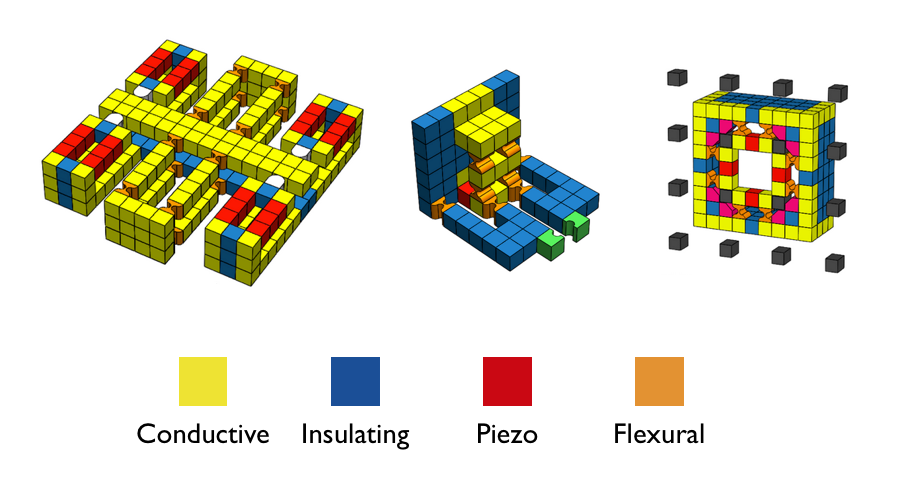
\includegraphics[width=\linewidth]{willMockups.png}
  \caption{Design mock-ups of assembler components made from digital materials by Will Langford.  From left to right: a linear actuator, a part gripping mechanism, a clamping mechanism.  None of these designs has been evaluated in simulation.}
  \label{fig:willMockups}
\end{figure}
The nano-assembly I've described will look very different from the way we make things today, and opposes many of the assumptions baked into traditional Computer Aided Design (CAD),  Computer Aided Manufacturing (CAM), and robotics.  This assembly strategy follows from an existing line of research called "digital assembly", where discrete parts are assembled on a regular, periodic lattice.  Mechanical systems are built with discrete modules of rigid and flexural components, and electronics and controls are distributed spatially across a machine (Fig \ref{fig:willMockups}).  Large structures appear to be "living" in the sense that their surface is teeming with nano-robots, detecting and correcting errors and performing other functions.  The environment is highly structured, allowing locomotion systems to position themselves globally by counting local movements across a lattice.  Machines receive instructions from their environment to coordinate various tasks.
\\

\section{Proposed Work}

I propose to build a design/simulation environment for digital materials based on realistic materials and physics, so that structures designed within this virtual environment may be physically realized one day.  I will use this virtual sandbox to design basic functional elements needed for the eventual goal of building a physically realizable assembler capable of self-replication.  Some elements of interest include mechanisms for grasping and moving parts in the assembler's environment, locomotion systems, information storage and retrieval, amplification, and digital logic.

\subsection{Part Types}

A major part of the initial phase of this project involves a literature review of research spanning biology, cellular automata, modular robotics, and materials science to pick the basis set of parts, their length scale, and a scheme for joining them together.  Initial sketches of the part types include rigid, flexure, piezo, conductive, insulating, capacitive, and resistive and scales ranging from $\mu$M to mm on a side.  The parts may become more complex for larger scales of bricks (transistors/logic gates).

\subsection{CAD Interface}

%\begin{figure}
%  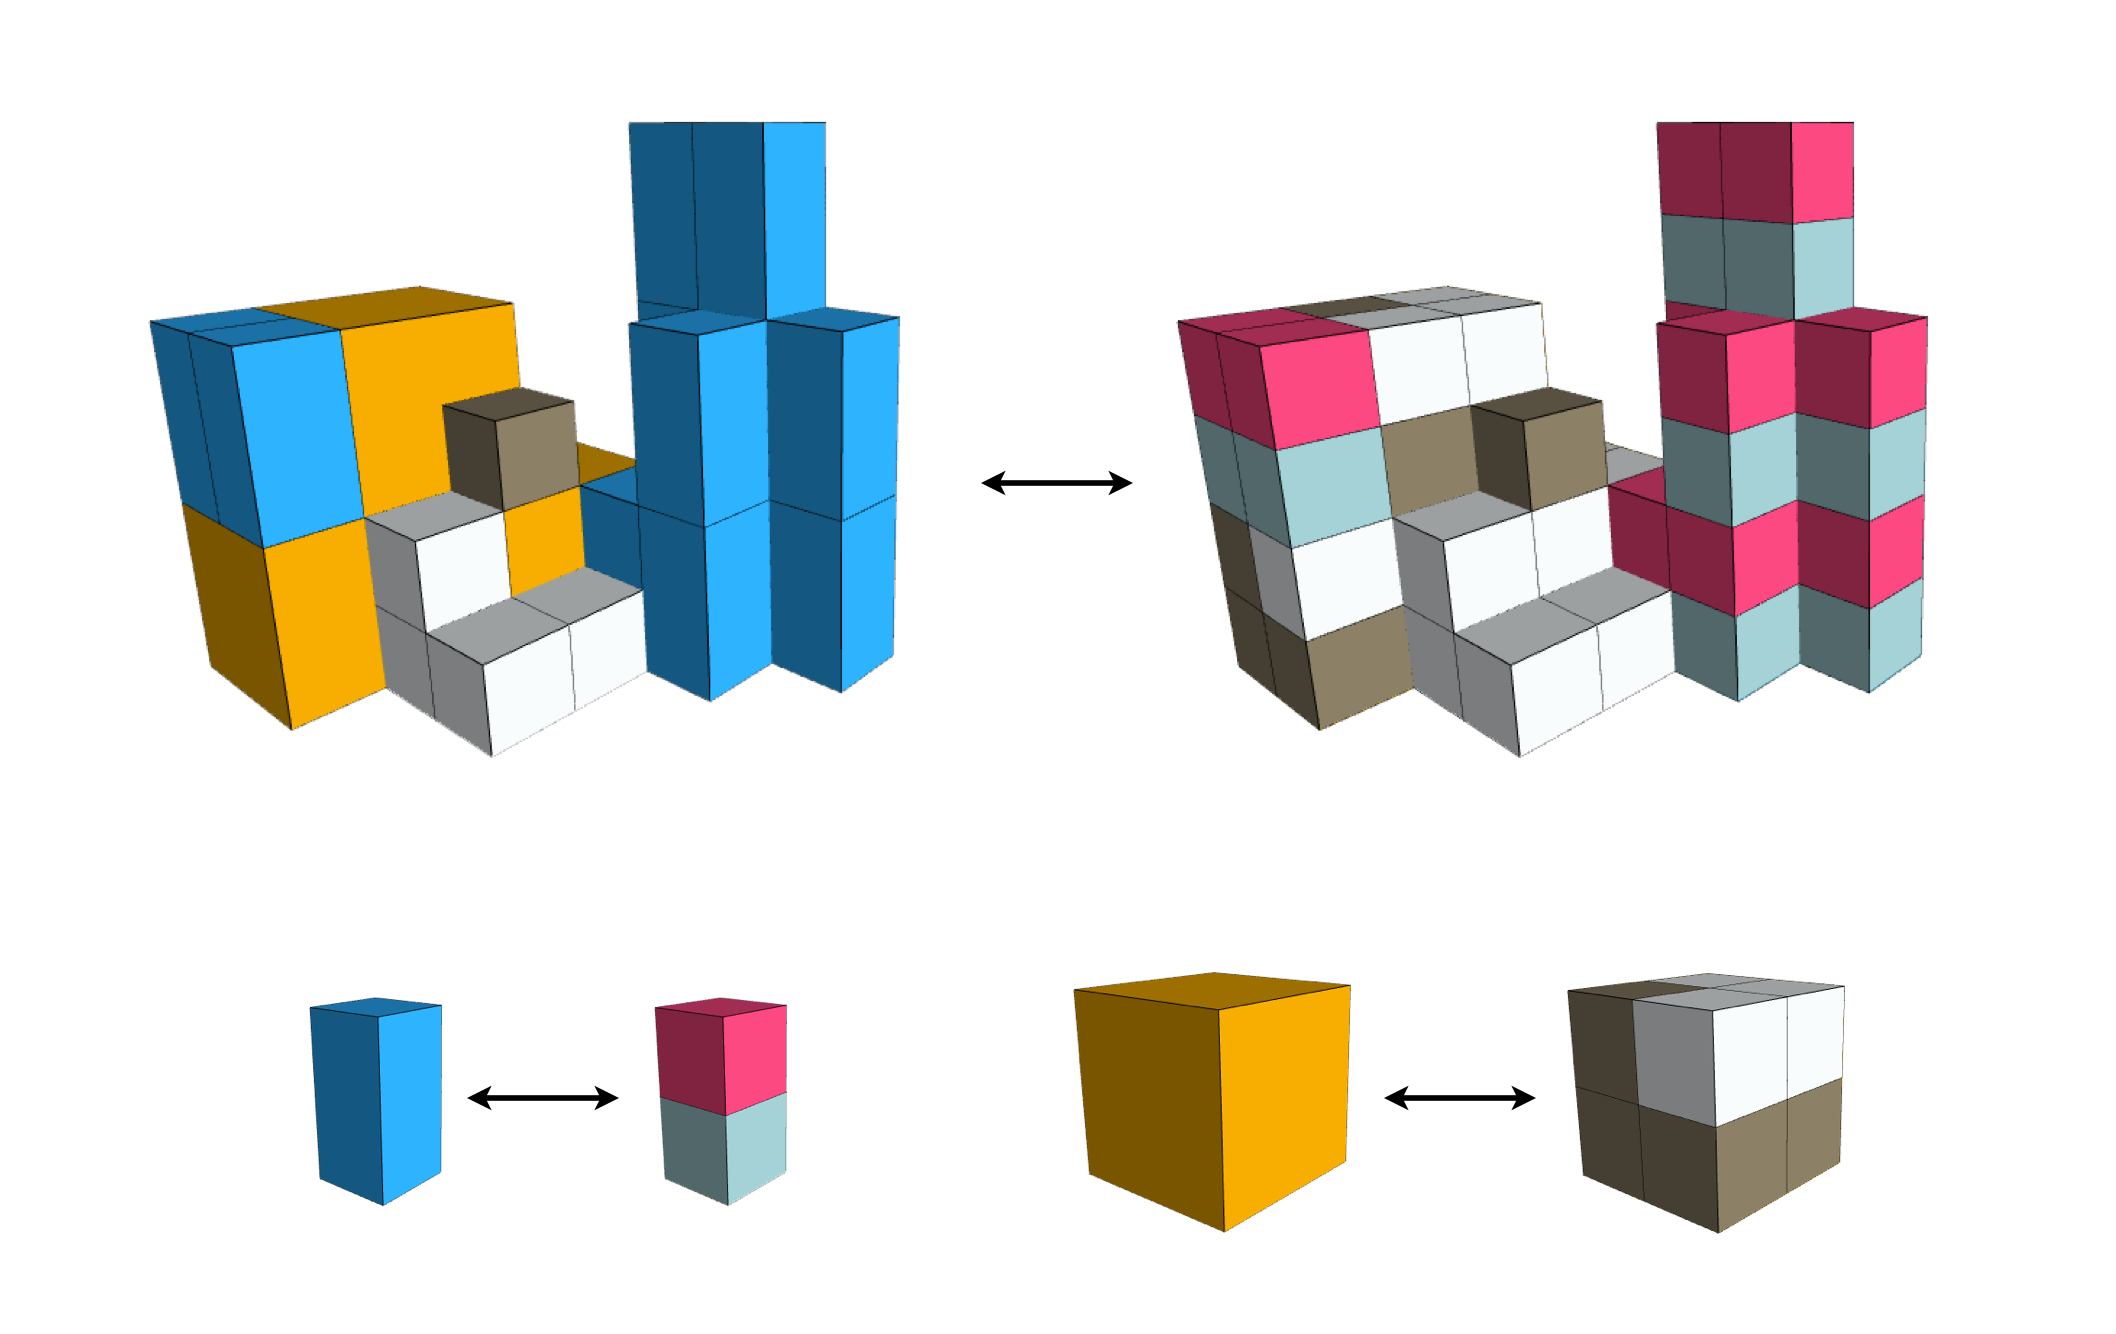
\includegraphics[width=\linewidth]{hierarchicalDecomp.png}
%  \caption{Hierarchical decomposition of lattice assembly. All hierarchical components are parametrically linked to a hierarchical material definition.}
%  \label{fig:hierarchicalDecomp}
%\end{figure}

Borrowing some classes and frameworks I've started in DMDesign, I will create a new project for the work spawned from this thesis.  All geometry will be assumed to fit on a regular cubic lattice, though flexural deformations may allow for off-grid motions.  Geometry will be represented in a hierarchical fashion (as is the case in DMDesign), where subassemblies of parts can be defined and patterned across a design, and all instances of a subassembly are linked parametrically to the same definition.

%\begin{figure}
%  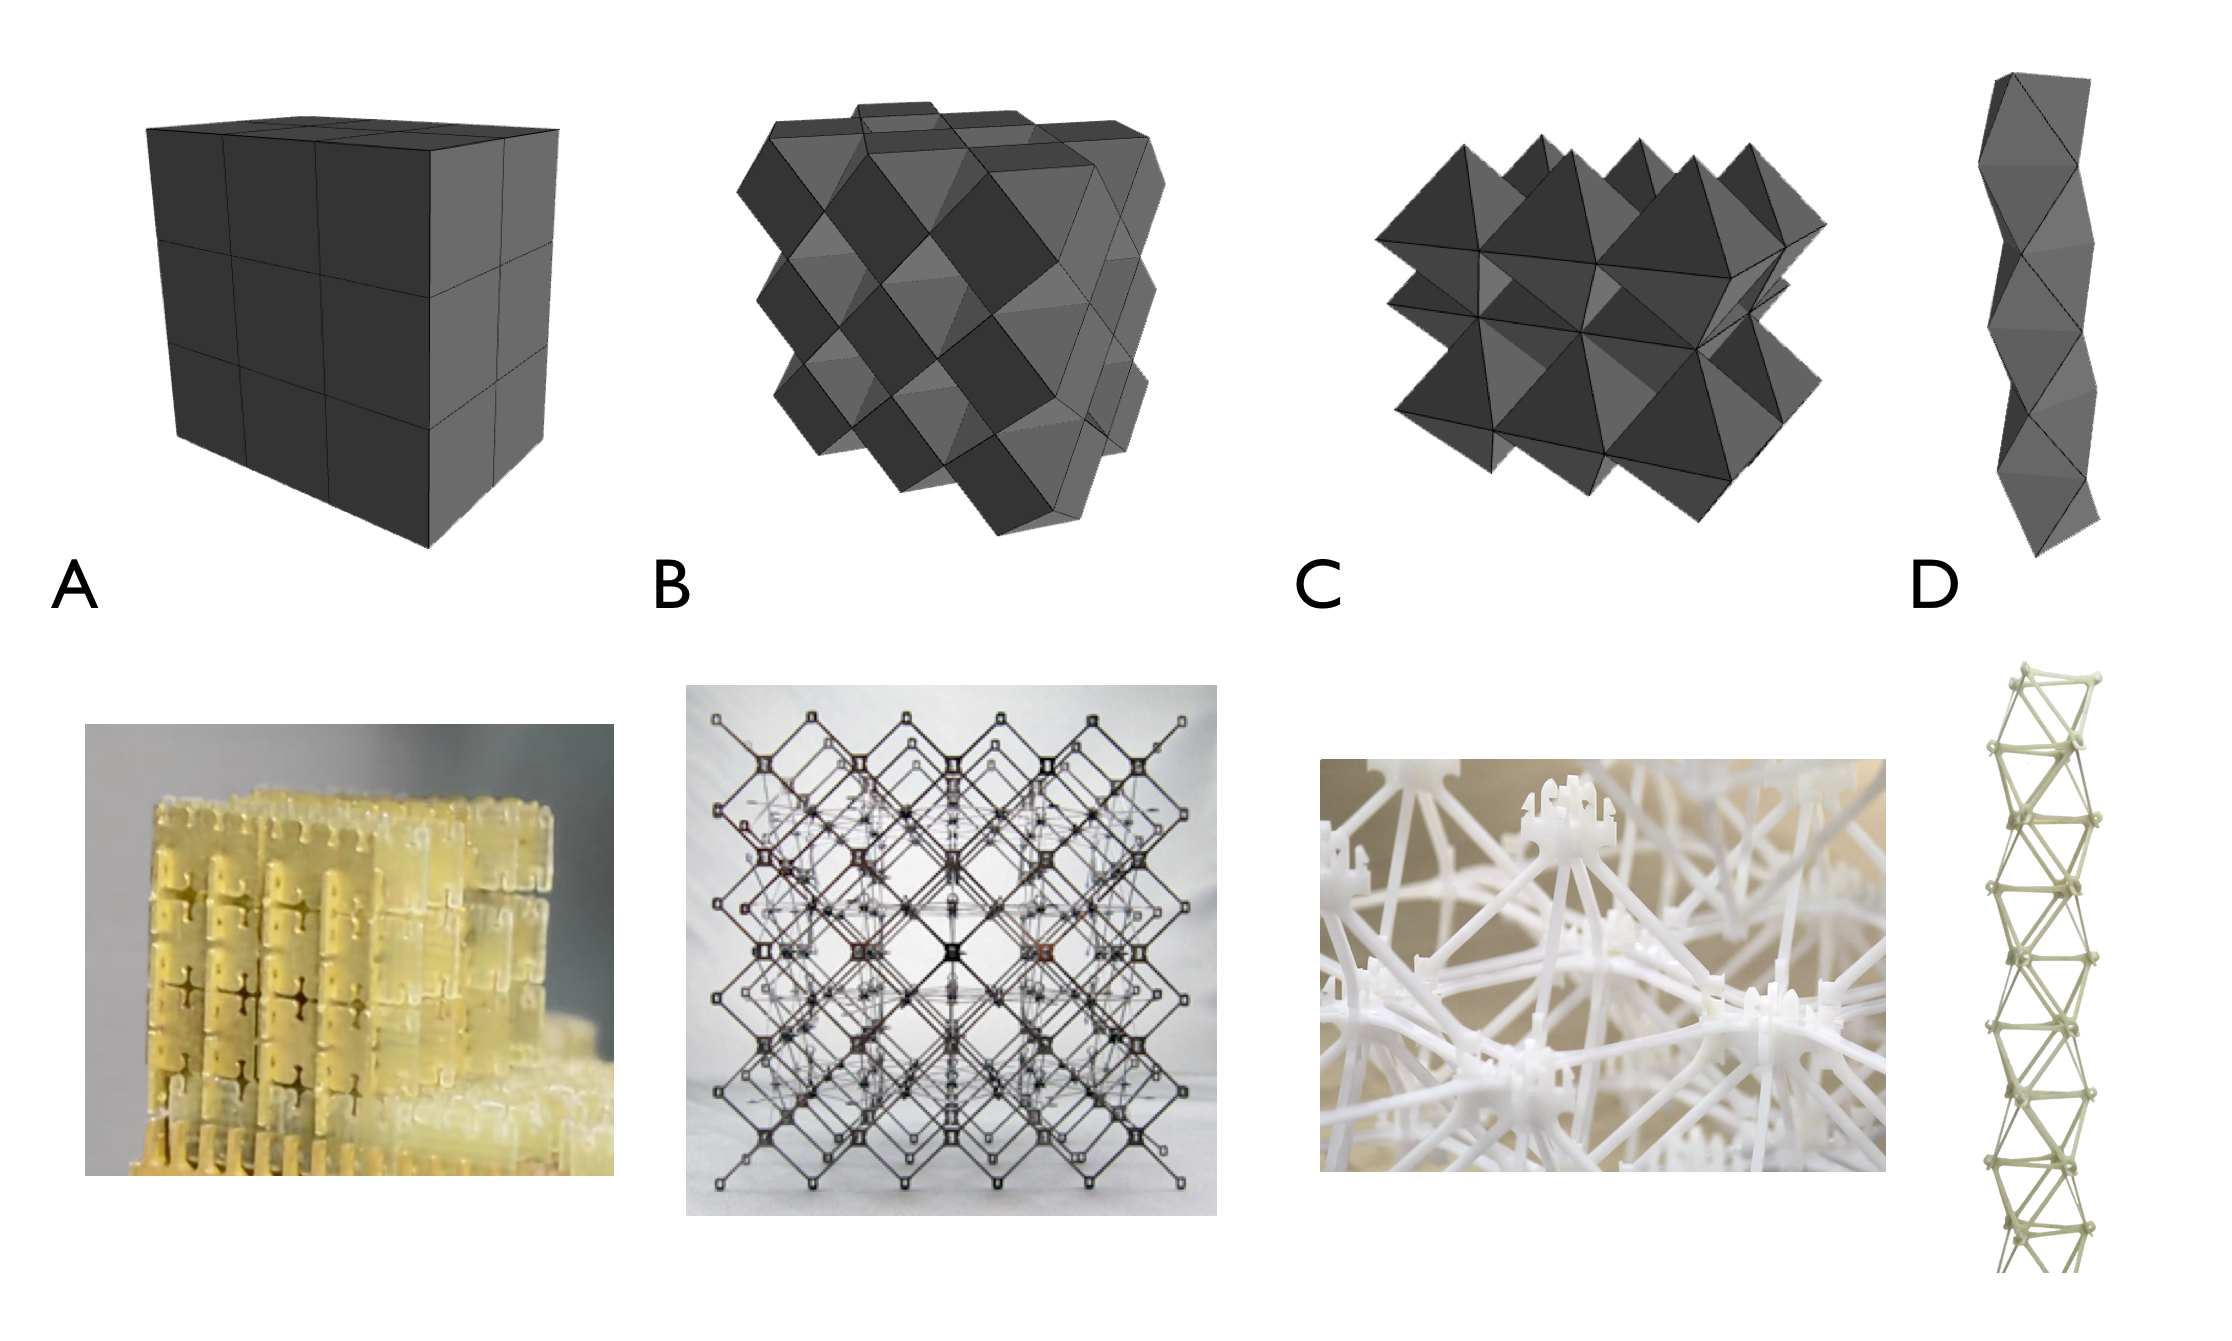
\includegraphics[width=\linewidth]{latticeVirtualRealComp.png}
%  \caption{Comparison of virtual lattice types with their real world counterparts.}
%  \label{fig: latticeVirtualRealComp}
%\end{figure}

%\begin{figure}
%  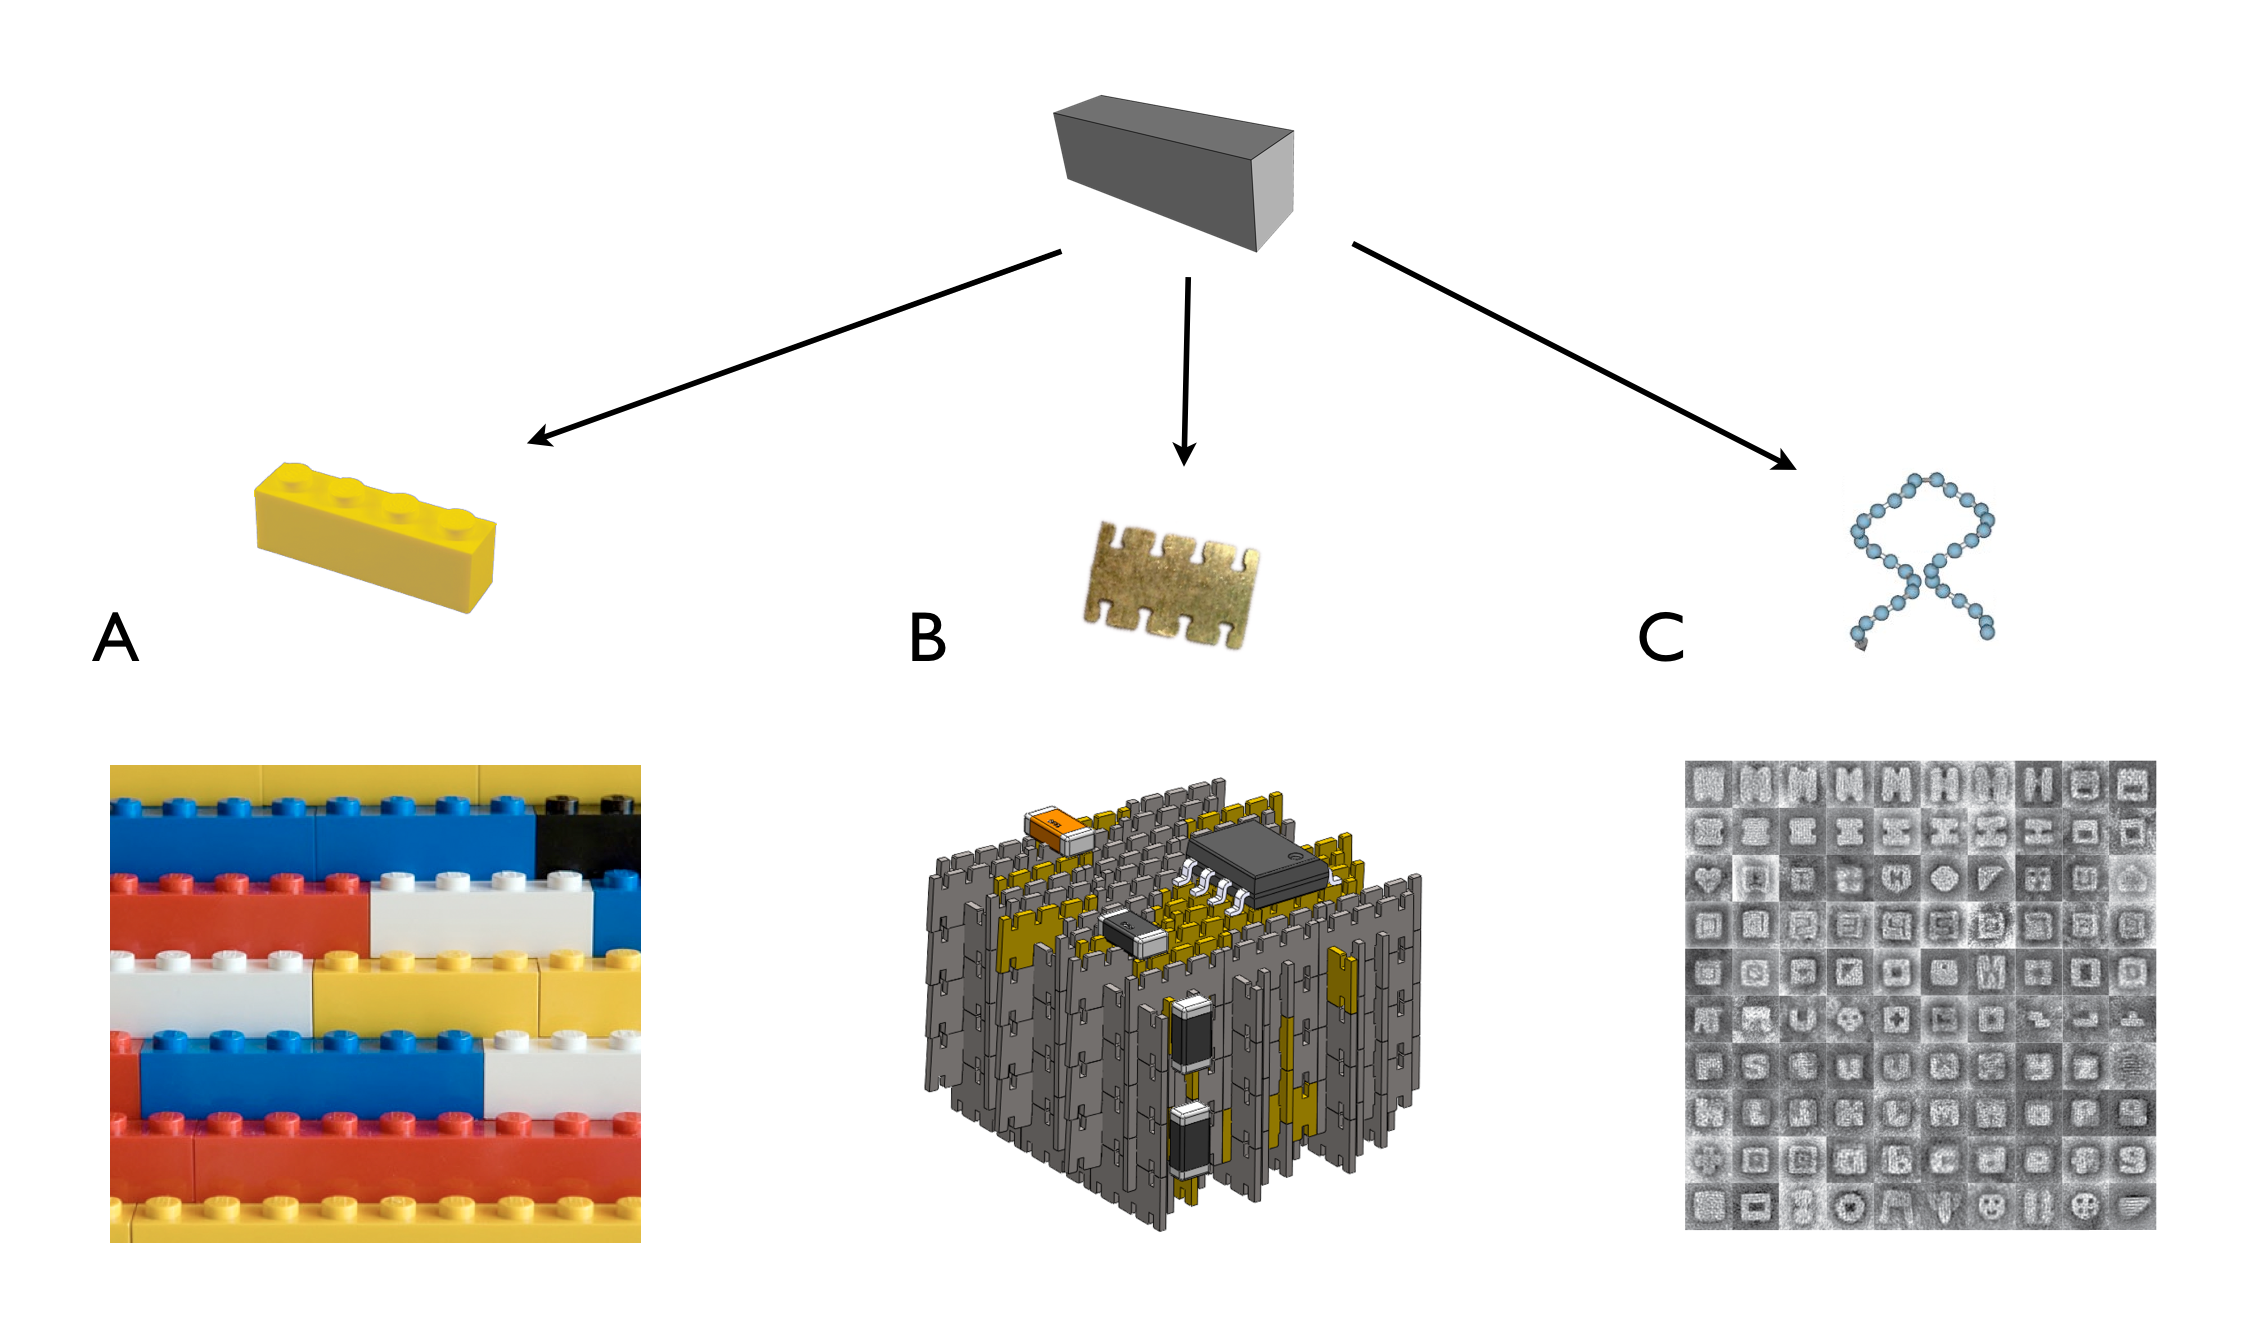
\includegraphics[width=\linewidth]{partAbstraction.png}
%  \caption{Part abstraction from lattice primitive.}
%  \label{fig: partAbstraction}
%\end{figure}

\subsection{Simulation Engine}

Dynamic simulation occurs at the granularity of the cell by modeling only local interactions between a cell and its immediate neighbors.  This way, as an assembly is designed through the CAD interface, its corresponding simulation model is constructed at the same time.  I hope that by implementing a local-only mode of simulation, I will be able to reuse the same connectivity model for both mechanical and electronic simulation, and cut down on computational costs.
\\

Locating parts on regularly spaced intervals on a lattice allows for computational shortcuts in simulation.  Depending on the nature of the mechanical and electronic simulation, I may be able to use a hash table to increase performance\cite{Gosper1984}, especially for repeating hierarchical structures within a model.  Previous work has adapted the hashlife algorithm for kinematic systems of cellular automata\cite{Stevens2010}.  I will surely need to spend some more time looking into this literature before implementing it in my own system.
\\

Additionally, I will need to implement some kind of collision detection for this system.  Due to the prevalence of gaming, there are an assortment of published algorithms to speed up  collision detection over the obvious naive approaches.  Many physics engines rely on a boundary representation of an object to detect collision with other boundaries - if objects are moving too quickly this can lead to unexpected results.  The voxels in my geometry will together define a volume of space, and the cells forming the boundary of this volume are known; I will leverage this to cut down the computational costs of collision modeling in my simulations.

\subsection{Approach}

The proposed digital materials sandbox will be built in Javascript using the following dependencies (more may be added):
\begin{itemize}
\setlength\itemsep{0em}
\item \href{http://threejs.org/}{Three.js} is a library that makes WebGL easy to use without sacrificing much in performance
\item \href{http://requirejs.org/}{RequireJS} is a framework for asynchronously loading javascript modules and dependencies
\item \href{http://backbonejs.org/}{Backbone.js} is a framework for managing UI events and giving structure to an interactive application
\item \href{https://jquery.com/}{JQuery} is a library that simplifies interactions with HTML and helps maintain cross-browser support
\item \href{http://underscorejs.org/}{Underscore} is a library with lots of useful functions for dealing with arrays and javascript objects
\end{itemize}

I know I will take some performance hit writing this application in JavaScript as opposed to a strongly-typed language like C running natively, but for this first implementation it makes sense to do start with a programming environment that I can rapidly develop in and experiment with.  If it turns out that I need to design very large structures in CAD or performance is getting in the way, I will consider porting the codebase into a compiled format.  With some optimization of the rendering, it is possible to render 100-200k voxels on the screen at 30fps in Three.js, it is unclear at this time exactly how costly the simulation will be.
\\

Aside from my own familiarity with web development, I'm interested in using HTML5/ Javascript for this application because it allows easier access to the code than any other platform.  Though user studies are not a component of this work, there is a long history of communities of users building things in these types of sandbox environments that surpass anything the developers were able to imagine.  There is a lot of talent beyond the immediate neighborhood of CBA, and I'd like to try to make this codebase as available as possible for anyone interested in exploring this new way of making things.

%\subsection{Assembly}
%
%\begin{figure}
%  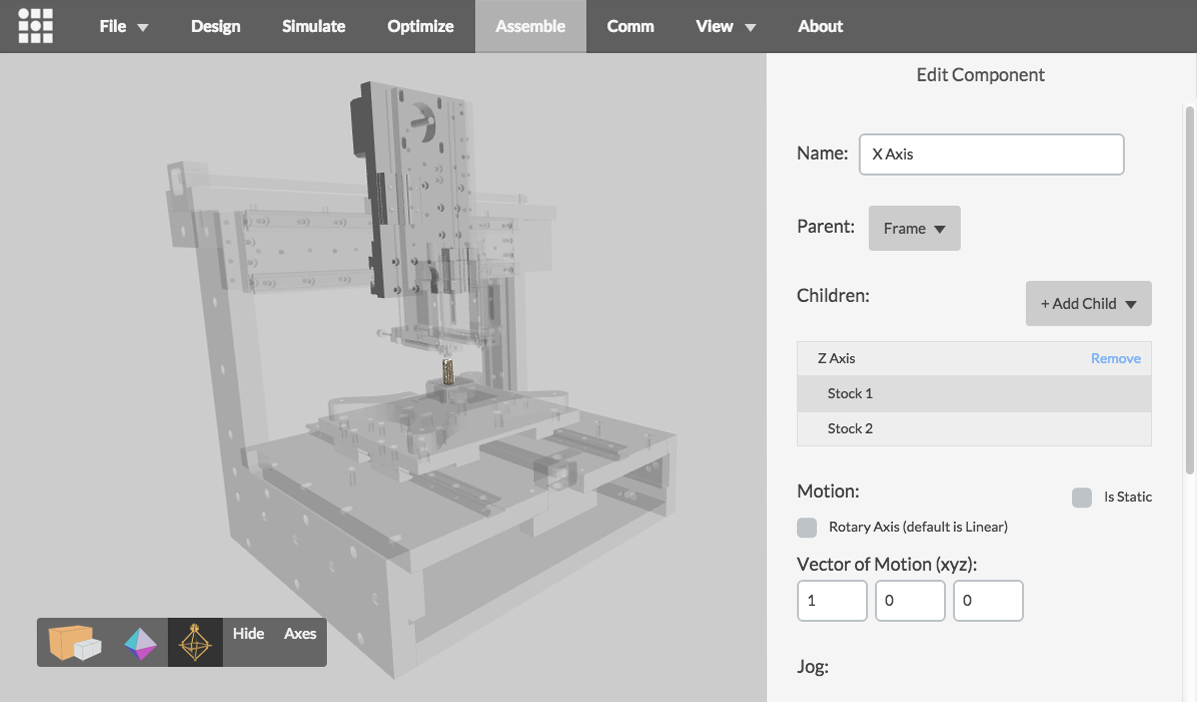
\includegraphics[width=\linewidth]{assemblerSetup1.png}
%  \caption{Screenshot of current assembler config GUI.}
%  \label{fig: assembleSetup1}
%\end{figure}
%
%\begin{figure}
%  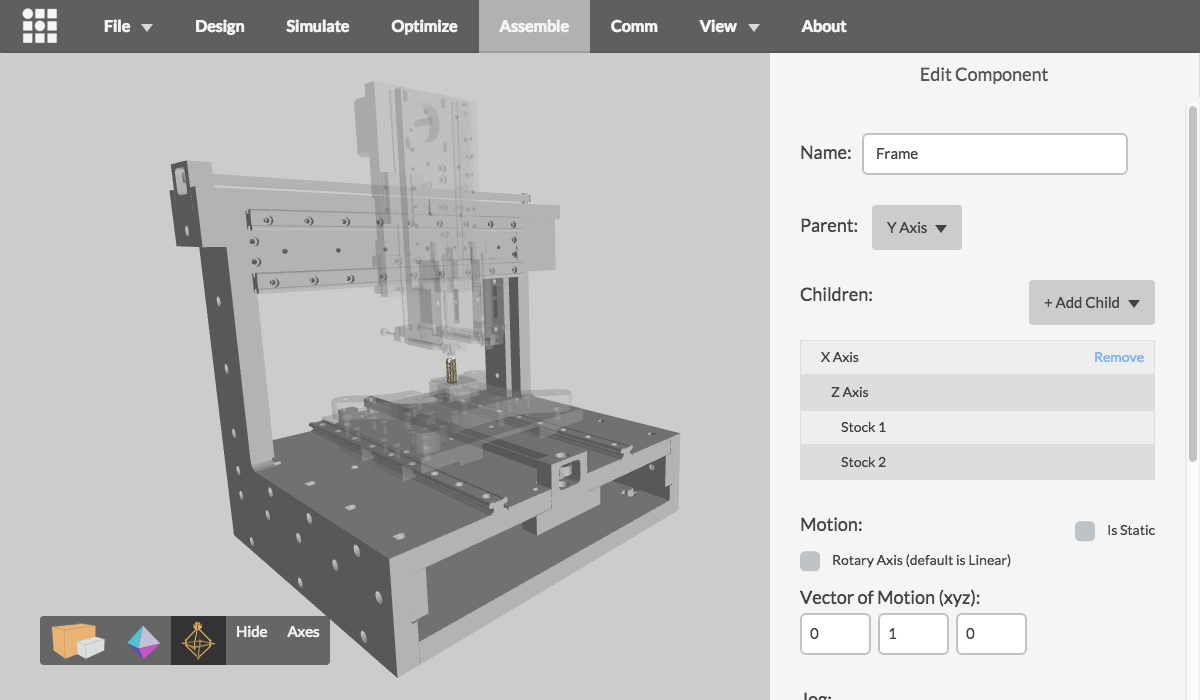
\includegraphics[width=\linewidth]{assemblerSetup2.png}
%  \caption{Screenshot of current assembler config GUI.}
%  \label{fig: assembleSetup2}
%\end{figure}
%
%urdf, tree description for abstraction
%calculate reverse kinematics
%abstraction of strategies and assemblers/low level operation

%\subsection{GUI}
%
%\begin{figure}
%  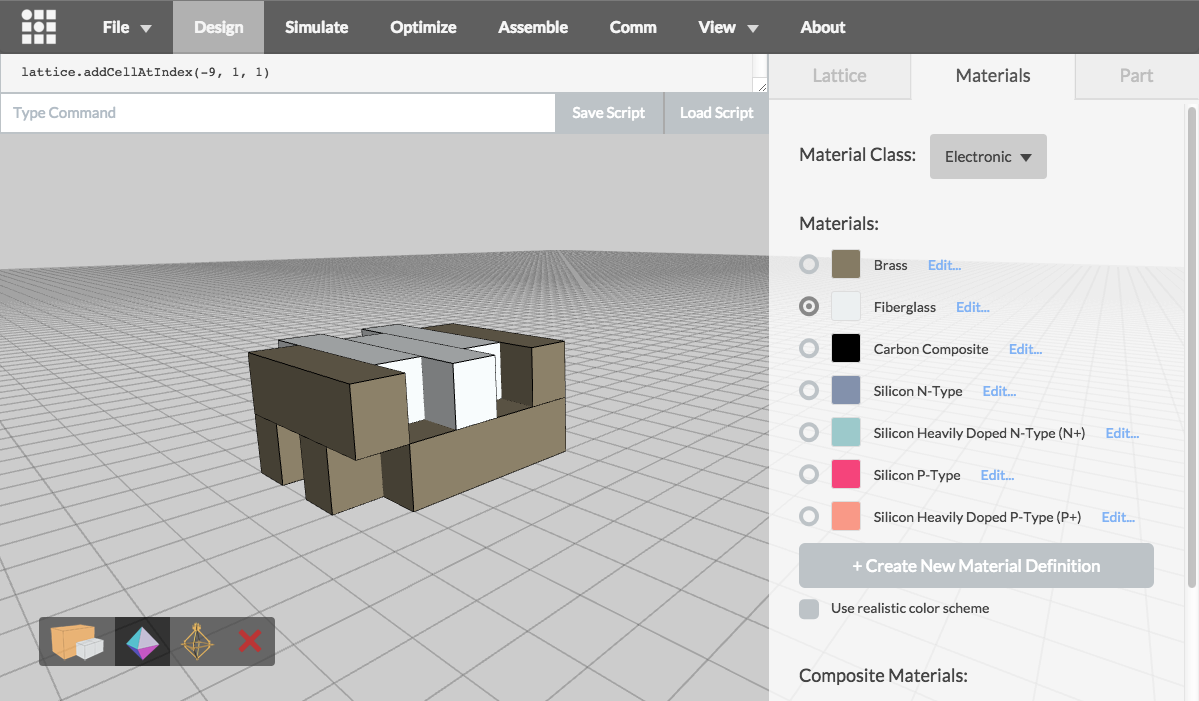
\includegraphics[width=\linewidth]{designGUI.png}
%  \caption{Screenshot of current design GUI.}
%  \label{fig: designGUI}
%\end{figure}
%
%\begin{figure}
%  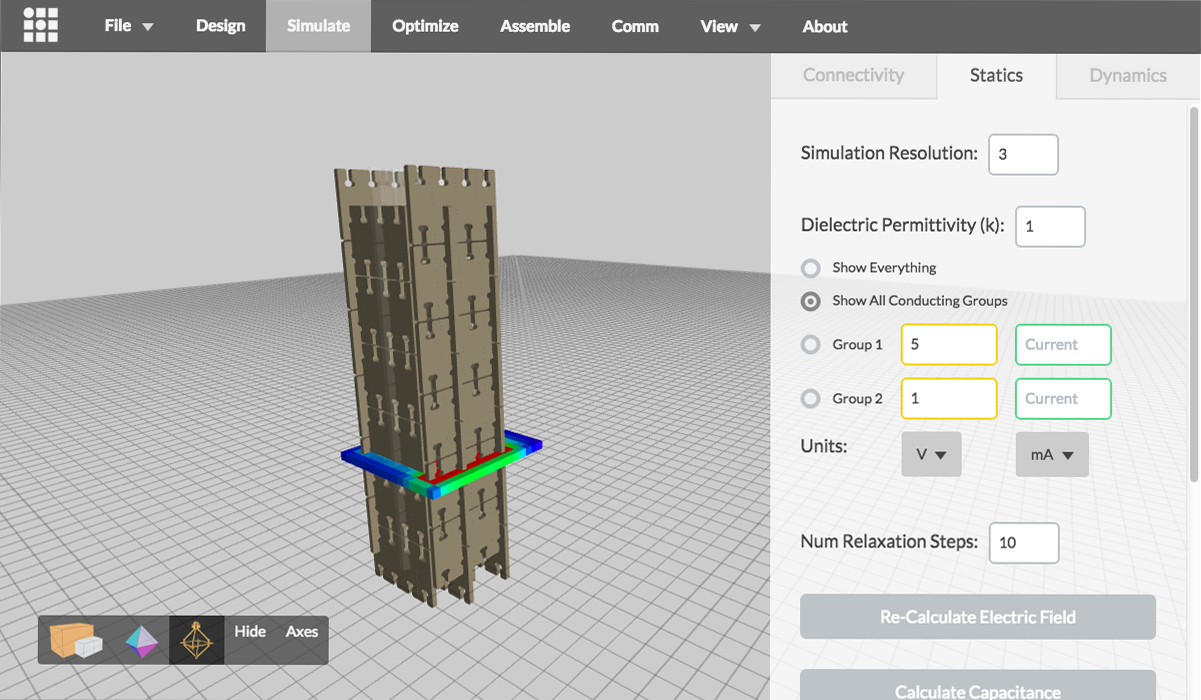
\includegraphics[width=\linewidth]{simGUI.png}
%  \caption{Screenshot of current simulation GUI.}
%  \label{fig: simGUI}
%\end{figure}
%
%\begin{figure}
%  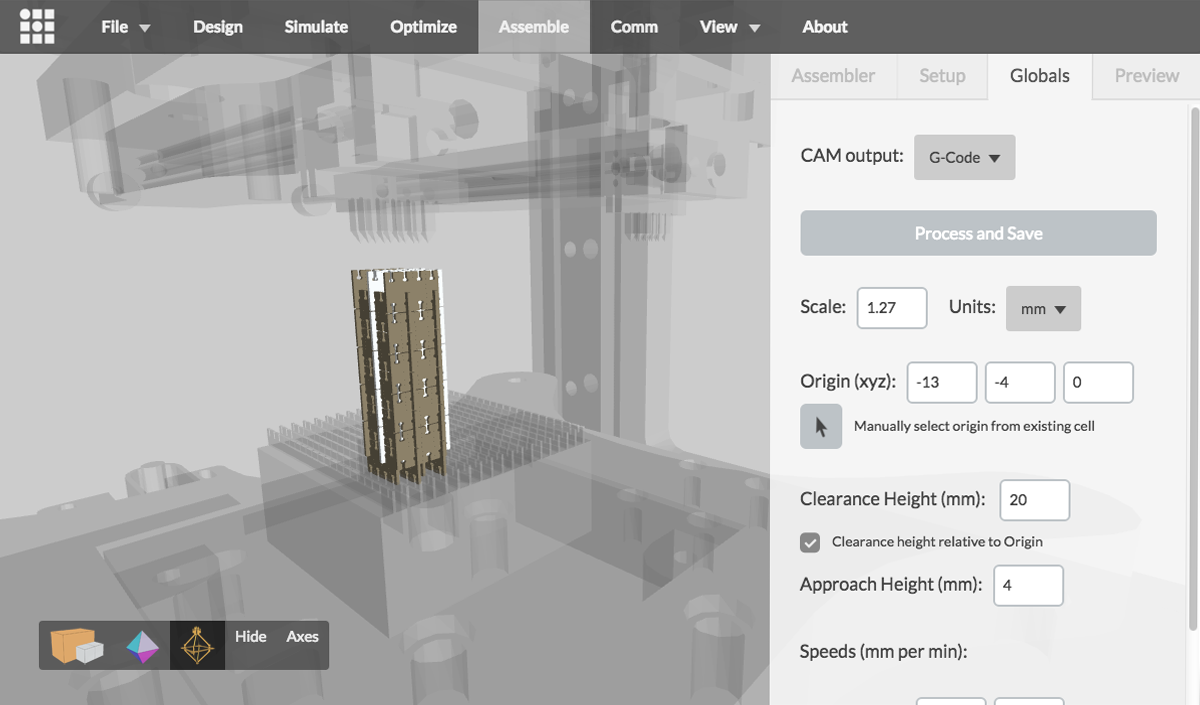
\includegraphics[width=\linewidth]{assembleGUI.png}
%  \caption{Screenshot of current assemble GUI.}
%  \label{fig: assembleGUI}
%\end{figure}
%
%javascript, etc, etc

%\subsection{API}
%
%Lattice, Cell, Material, CompositeMaterial classes.
%
%\begin{figure}
%  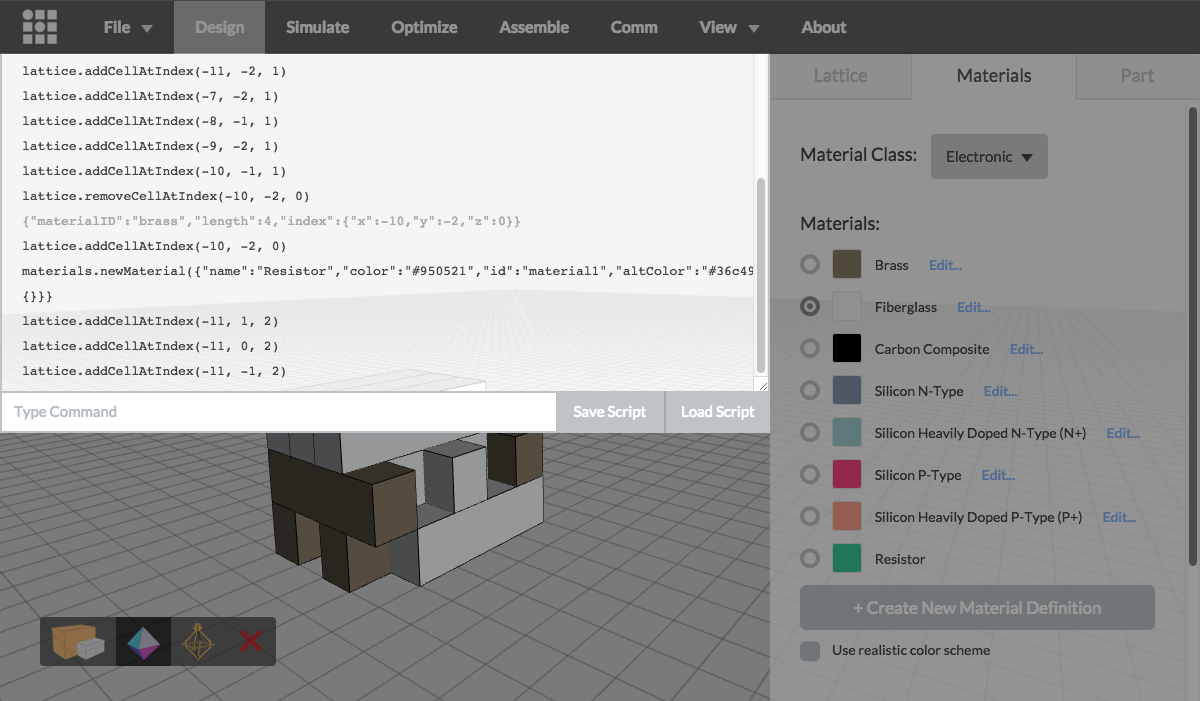
\includegraphics[width=\linewidth]{scriptGUI.png}
%  \caption{Screenshot of current script GUI for API with scripting console highlighted.}
%  \label{fig: scriptGUI}
%\end{figure}
%
%asdfdsf

\section{Contribution}

As outlined in previous sections, the main contribution of this work is to create a design/simulation environment where anyone can start to explore the rich design space around digital materials in a physically realistic way.  This work will inform future trajectories in CBA research and in the broader field of programmable materials, modular robotics, and digital fabrication.  This work is not intended to result in a manual outlining all the necessary components for self-replication based on current technology, but rather as an sandbox for exploring self-assembling systems based on the foundations of engineering and materials science rather than biology.

\section{Evaluation}

Once the CAD/simulation environment is set up, I will design several functional objects within it and evaluate their function both quantitatively and qualitatively.  Some objects that would be especially interesting include:
\begin{description}
\setlength\itemsep{0em}
\item[] locomotion systems
\item[] end effectors (gripping mechanisms, part manipulation)
\item[] information storage and retrieval
\item[] amplification of motion and signals
\item[] digital logic
\end{description}
Qualitative assessment includes evaluation of success or failure of the intended function (can a gripping mechanism grip a part), and quantitative assessment includes calculations of performance (gripping strength, speed of locomotion, volume required to implement various types of digital logic, speed of memory access, etc).

\section{Resources Required}

The majority of the work involved in this thesis will happen in the computer and require no material resources.  If required, I will use CBA's cluster for highly parallel computational operations.  Fabrication of assemblers and parts to be used in the digital assembler workflows should be considered outside the scope of material resources required by this thesis, and will be supplied by CBA.

\section{Schedule}

\begin{description}
  \item[11/6/15]\tabto{1.5cm}Proposal Due
  \item[11/9/15]\tabto{1.5cm}Crit Day Presentation
  \item[11/15]\tabto{1.5cm}Design and assembly workflow for digital materials is in a working state.  I will use elements of the classes and framework developed in that project to begin a new project specifically for the completion of the thesis.  This new project will only be concerned with the design and simulation of multimaterial assemblies on a cubic lattice (for simplicity).  Finish CAD interface.
  \item[12/15]\tabto{1.5cm}Hello world of basic CA behind the electronic/mechanical simulation.  Not worrying about efficiency at this point, get cells moving and communicating.  Start making decisions about scale and part types, num materials, geometry, allowed interactions, interfaces.
  \item[1/15]\tabto{1.5cm}Build out main components of simulation engine.
  \item[2/15]\tabto{1.5cm}Collision detection strategies, unconnected modules should be able to interact with each other
  \item[3/15]\tabto{1.5cm}Refinement and optimization of simulation engine
  \item[4/15]\tabto{1.5cm}Performance optimization and design studies
  \item[5/15]\tabto{1.5cm}Design studies and writeup
  \item[6/6]\tabto{1.5cm}Thesis Due
\end{description}

}

%%% This is an example first chapter.  You should put chapter/appendix that you
%% write into a separate file, and add a line \include{yourfilename} to
%% main.tex, where `yourfilename.tex' is the name of the chapter/appendix file.
%% You can process specific files by typing their names in at the 
%% \files=
%% prompt when you run the file main.tex through LaTeX.

\singlespacing{

\chapter{Related Work}\label{chapter:RelatedWork}


The following sections outline current research into discretely-assembled construction platforms across scales and CAD/simulation packages which occupy a similar space to what I have built.
%

\section{Programmable Materials}

Programmable matter describes materials that can be programmed to change their physical properties based on user input or environmental changes.  Often, programmable materials are composed of many smaller constituent elements, whose structural arrangement and local interactions are the source of larger-scale programmable properties.  Some forms of programmable material include metamaterials \cite{Smith2000} \cite{Khorasaninejad2016}, modular robotics \cite{Rubenstein2014} \cite{Romanishin2015}, and shape-changing materials \cite{Zhao2016} \cite{Hawkes2010} \cite{Tibbits2014}.  Programmable matter may also describe computing systems, for example CAM8 is a computing architecture in which physical phenomena can be efficiently simulated based on local interactions between parallel computing elements \cite{Toffoli1991}.

\section{Digital Materials and Digital Assembly}
Current research at CBA revolves around a discretely-assembled form of programmable matter called \textit{digital materials}.    Digital assembly is an emerging multimaterial fabrication technique where a finite set digital materials are (often reversibly) joined to form larger structures in a regular lattice.  Programmable functional behavior is achieved by patterning parts with different material properties across an assembly.  The assembly process is orchestrated by one or many robotic assemblers.  The regular spacing of the parts minimizes the complexity of the assembly design, the robotic assemblers that locomote across the lattice, and the ``path planning'' strategies for assembly.  Self-alignment features on the digital material parts maintain global metrology through local interactions; a robotic assembler can construct a structure more precise than itself, within a certain error tolerance.  At nano scales, assembly may be guided by programmable self-assembly mechanisms.  Chapter \ref{chapter:HierarchicalDesign} describes hierarchical scaling of complexity within digital assemblies.  

\subsection{Macro Assembly}

Cheung showed that carbon fiber composite parts can be reversibly assembled to form ultralight materials for aerospace applications \cite{Cheung2013}.  Programmable flexibility is achieved by pattering rigid and flexural parts across an assembly and also by varying the density and connectivity of the parts.  Additional research into digital assembly of structural elements is ongoing at CBA, including modeling of the parts and assemblies using finite element analysis \cite{Calisch2014} and designing new part geometries and robotic assemblers \cite{Carney2015}.

\subsection{Micro Assembly}

\begin{figure}
  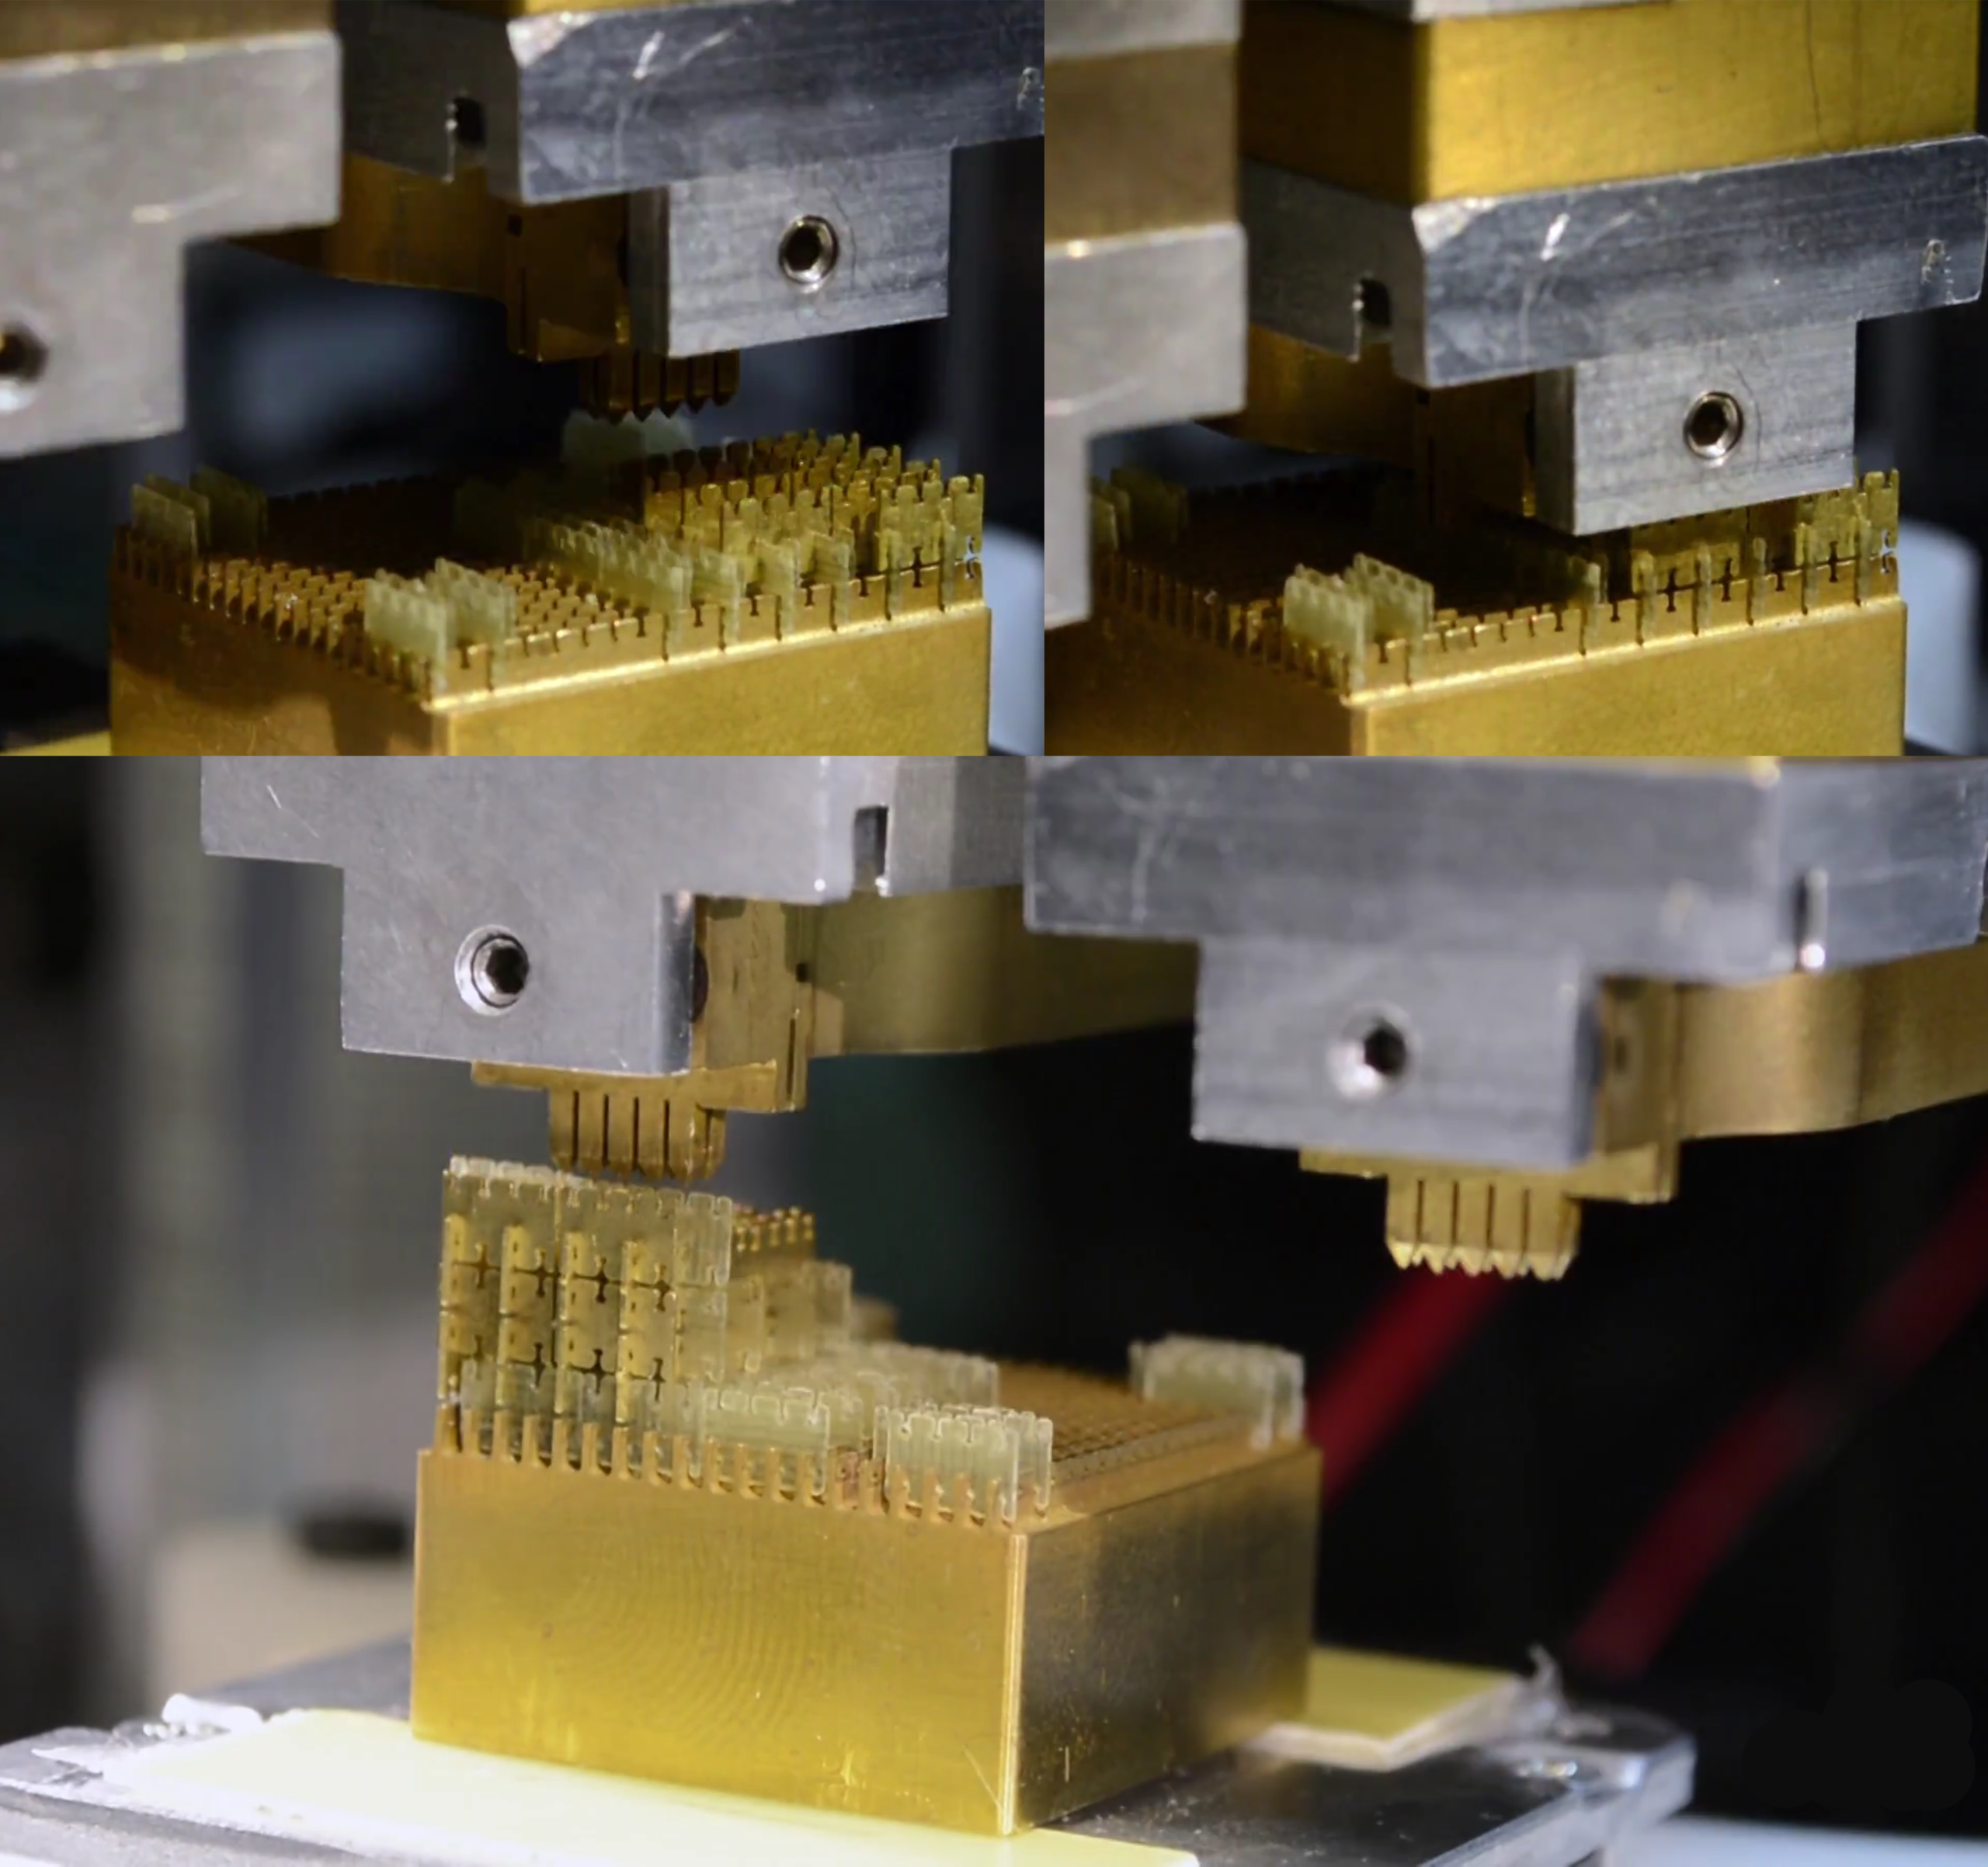
\includegraphics[width=\linewidth]{willAssembler.png}
  \caption{``Stapler'' assembler designed by Will Langford assembles conductive and insulating discrete part types to form electronic structures with tunable capacitance and inductance.  \textit{Image Credit: Will Langford 2015}}
  \label{fig:willAssembler}
\end{figure}


%\begin{figure}
%  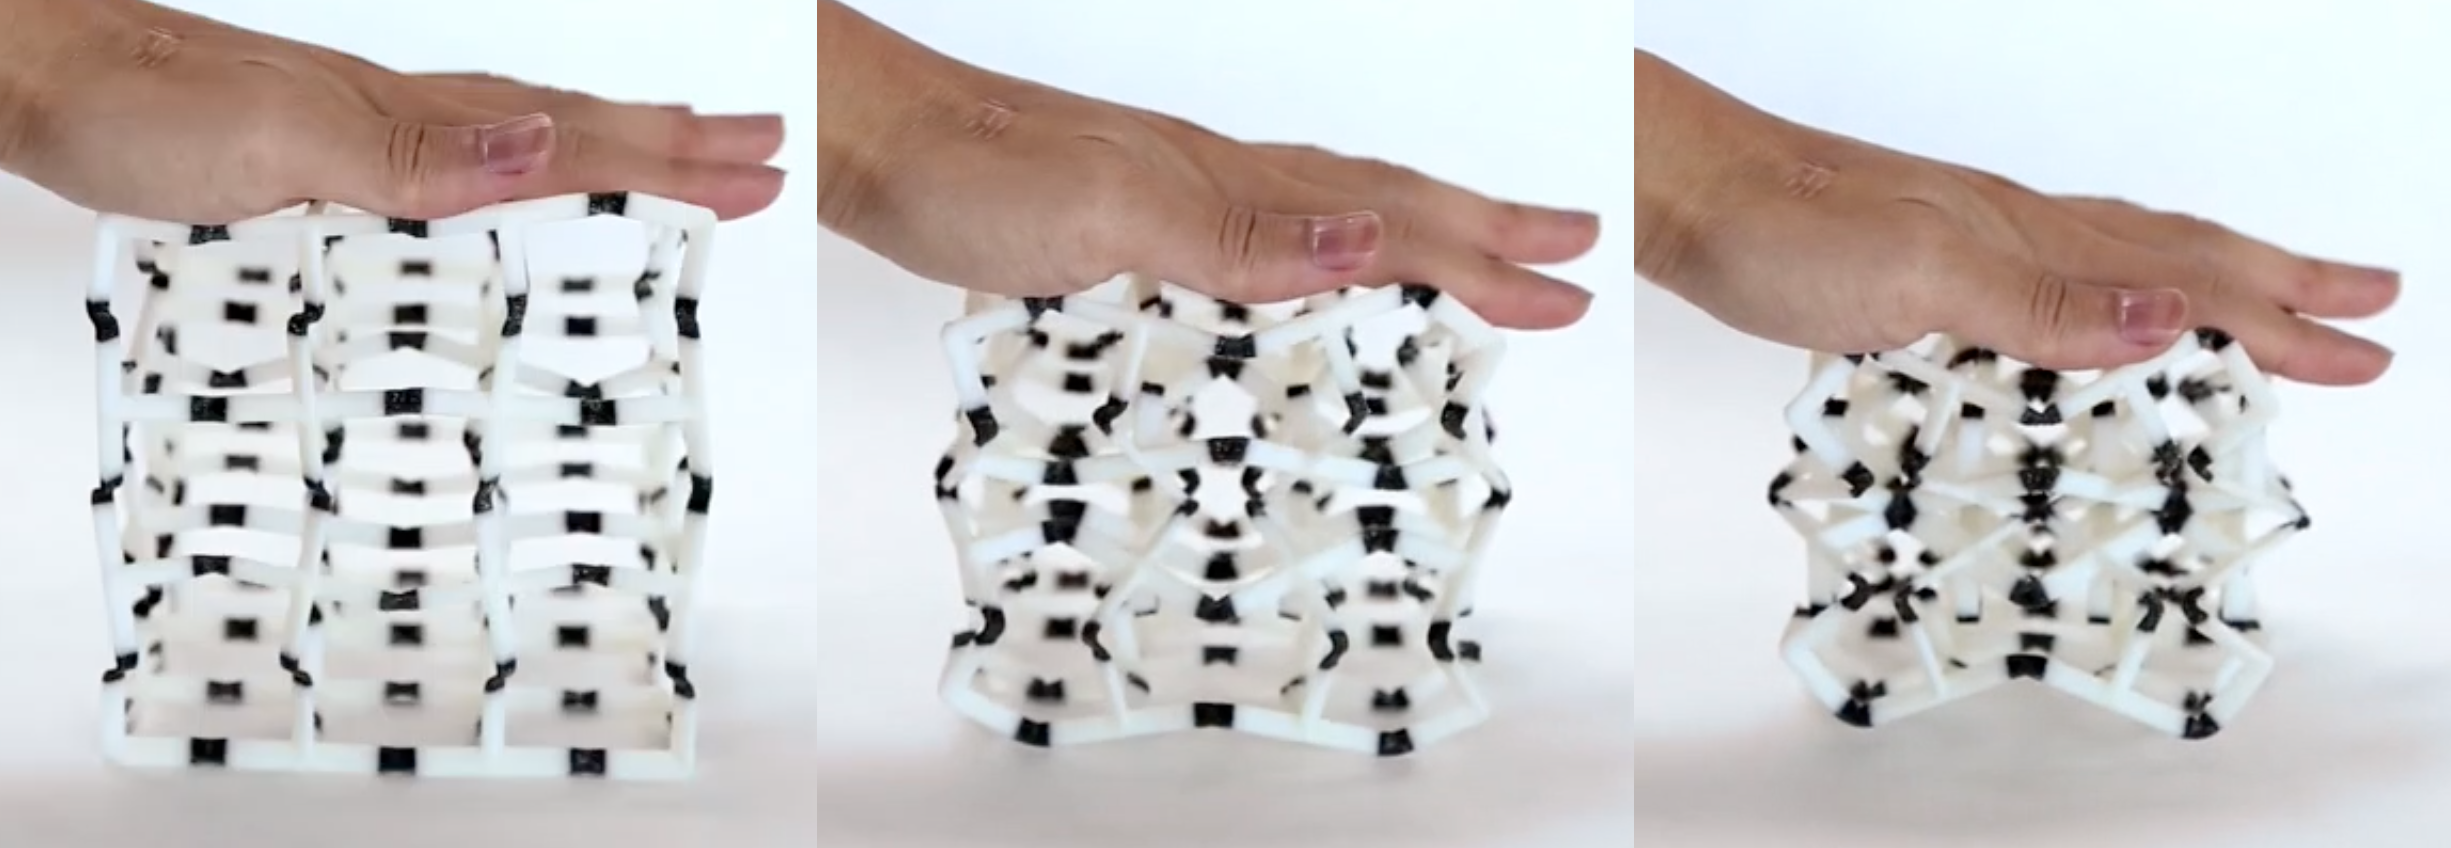
\includegraphics[width=\linewidth]{objetMultimaterial.png}
%  \caption{Mechanical properties programmed by material deposition in Objet 3D print.}
%  \label{fig: objetMultimaterial}
%\end{figure}

Langford demonstrated how conducting, insulating, and resistive part types ranging in scale from mm-$\mu$m could be assembled to form any passive electronic component, including antennas and RF matching networks \cite{Langford2014}.  Langford designed and built a dual-material assembler (Fig: \ref{fig:willAssembler}) for constructing passive electronic structures from conducting and insulating parts (\href{http://dma.cba.mit.edu/stapler/video/dualstapler_full_1.mp4}{video}) \cite{LangfordWillGhassaeiAmandaGershenfeld2016}.  Langford suggests that by extending the part types to include several types of silicon components, discretely-assembled active components like diodes and transistors would be possible.  Work toward the fabrication and realization of these silicon components is ongoing.  This work follows from previous work by Popescu et al. on reversibly assembled ``GIK'' structures spanning many length scales and material types \cite{Popescu} and also work by Ward on discretely assembled electronics \cite{Ward2010}.
\\

Hiller et al. propose a method of additive manufacturing using multimaterial voxel building blocks \cite{Hiller2009a}.  They explore various voxel decompositions of 3D geometry and assess their suitability for rapid, parallel assembly processes (\href{https://www.youtube.com/watch?v=-szjlhVMGh4}{video}).  Possible applications discussed include desktop manufacturing, especially for electromechanical and microfluidic devices.  Hiller et al. also propose reversible processes for disassembling voxel assemblies back into their constituent parts \cite{Hiller2005}.
\\

Though not a reversible process, multimaterial 3D printing (most notably by the Objet printer) deposits material in voxels on the order of ~10$\mu$m$^{3}$ with a total build volume on the order of 1x10$^{10}$ voxels \cite{Objet1000}.  Multimaterial 3d printing has been demonstrated in optical \cite{Willis2012}, electronic \cite{Ahn2009}, and structural applications \cite{Skouras2013} \cite{Schumacher} \cite{Bacher2014}.

\subsection{Nano Assembly}

``DNA bricks'' is a method of discrete nano-assembly based on complementary base pair interactions of short segments of DNA \cite{Ke2012}; DNA bricks forms a branch of a field called DNA origami \cite{Rothemund2006} or DNA computing \cite{Seeman1982} \cite{Adleman1994}.  The brick assemblies have a spatial resolution of 2.5nm; the longest dimension of a DNA brick assembly measures on the order of 1$\mu$M \cite{Ke2014}.  Unlike the previously discussed processes, assembly of DNA bricks takes place through passive, stochastic interactions between DNA strands in solution, rather than guided assembly by robotic assemblers.
\\

CBA is actively involved scaling down the micro-electronic parts designed by Langford \cite{Langford2014} into the nanoscale and assembling them using nano-manipulation devices.

\section{Self-Replication}

Some of the first known formal investigations into the nature of self-replicating systems were conducted by John Von Neumann as early as the 1940s.  Since then, both physical and virtual self replicating systems have been explored by researchers in robotics, nanotechnology, biology, and computer science, as well as by a community of enthusiasts.\\

%\subsubsection{Construction vs Computation}
%
%If a system is able to perform universal computation and universal construction, it has the ability to self-replicate.  The reverse statement is more complicated.  Some self-replicating systems
%
%In order to prove universal computation, a system must exhibit the following properties:
%\begin{itemize}
%  \item Infinite memory
%  \item Clock
%  \item Data transmission mechanism
%  \item Universal boolean logic (AND and NOT gates are sufficient)
%\end{itemize}


Within the study of self-replication, there is a distinction between so called ``trivial'' and ``non-trivial'' self-replication.  This distinction is not well formalized; it is loosely based on the difference in complexity between a self replicating system and the parts it's constructed from.  For example, crystal growth or polymerization could be considered a type of trivial self-replication because both the assembly and the parts are relatively simple.  Penrose Tiles \cite{Penrose1958} are an example of trivial, artificial self-replication that resembles crystallization.  On the other end of the complexity spectrum, self-replicating experiments in the field of modular robotics also fall in the category of trivial self-replication; though the self-replicating robots produced in these experiments are very complex  \cite{Zykov2005} - often with multiple actuated degrees of freedom - the modules they're made from are of essentially equal complexity.

\subsection{Physical Self-Replicating Systems}

Biological self-replication is the only physically-instantiated, non-trivial self-replicating system that is currently known to exist.  The field of molecular biology aims to understand structure and functions of this system better, and the field of abiogenesis aims to discover how it first began.  An active area of synthetic biology explores the possibility of creating a viable cell from scratch based on knowledge about the core systems required for metabolism, cell maintenance, and self-replication \cite{Forster2006}.  To date, efforts at creating this ``minimal cell'' have been successful using a top down approach - starting with an organism with a minimal genome and reducing its genes further \cite{Glass2006} \cite{Gibson2010} \cite{Iii2016}.  Chapter \ref{chapter:HierarchicalDesign} dives deeper into an explanation of biological self-replication in terms of the work described in this thesis. 

%Other proposed non-trivial self-replicating systems include Drexler's mechanical nanobots  \cite{aSDASD} and self-replicating lunar factories \cite{adas}, others? though these have gained little traction from mainstream science.
%Some proposed non-trivial self assembling systems are Drexler's Mechanical Nanobots
%https://en.wikipedia.org/wiki/Drexler%E2%80%93Smalley_debate_on_molecular_nanotechnology
\subsection{Virtual Self-Replicating Systems}

This thesis draws inspiration from a lineage of virtual environments wherein the first investigations of self-replication took place.  Early experiments were computed by hand on pieces of graph paper or a Go board \cite{Gardner1970}.  With the introduction of personal computers and graphical user interfaces, it is now possible for anyone to compute large virtual universes and study the behaviors of millions of interacting parts.

\subsubsection{Cellular Automata}

A cellular automaton (CA) is a discretized model used to describe the dynamics of a system.  CAs are discrete in both space in time, meaning space is divided up into many identical \textit{cells} and time moves forward in discrete \textit{steps}.  Each cell owns one or many state variables, which may hold discrete or continuous data.  The governing equations of a CA system are codified in the ``ruleset'' that applies universally across all cells in the system; typically a ruleset describes local interactions of a cell with its neighbors.  For example, in the popular CA \href{https://en.wikipedia.org/wiki/Conway's_Game_of_Life}{Conway's Game of Life}, the state of a cell in the next time step is a function of its current state and the state of its eight neighbors on a 2D grid.  Some CAs consider cells to be spatially static with changing state, others employ kinematic rules, where cells can move across space.\\

CAs have been used to study the requirements of self-assembling systems since Von Neumann's first experiments \cite{Neumann1966}.  To date, CA investigations into self-replication have employed very simple rulesets that violate basic physical principals: matter can be created and destroyed at will, actuators can move an infinite number of cells (cells have no mass), motions are quantized, one material can be converted into another, global synchronicity, etc.  This does not imply that CAs are inherently non-physical; in fact, evaluating partial differential equations from physics using finite difference method can be structured of as a type of CA \cite{Yang2010}.

\subsubsection{Von Neumann's Universal Constructor}

A universal constructor is a machine that can be programmed to construct nearly any other structure, including a copy of itself.  In the 1940's Von Neumann designed a virtual CA world in which he built a universal constructor from 29 distinct parts types with discretized state and behaviors (this work was published posthumously by Arthur Burks in the 1960s \cite{Burks1969}).  A few notable conclusions fell from this exploratory investigation:\\

\begin{itemize}
\item{A distinction between the mechanistic parts of the constructor and the data encoding its construction (the ``blueprint'') - mirroring the separation of DNA from the proteome.}
\item{Establishing that bimodal operation of the construction blueprint is needed to make self-replication possible.  The blueprint must operate in both an interpreted mode - where it is read and executed to build mechanistic components - and a duplication mode - allowing its information to be copied bit by bit.  This insight predated the discovery of the structure of DNA and a formal understanding of DNA transcription and replication.}
\end{itemize}
%Other notable works that fall from Von Neumann's universal constructor include Langton Loops\cite{}...and more

\section{CAD and Simulation Tools for Digital Assembly}

At the moment of writing this, there exist several computational tools for designing and simulating static and kinematic, discretely-assembled structures.

\subsection{Cellular Automata-Based Tools}

The CA-based simulation tools discussed here allow for computational efficiency at the cost of accuracy, often using quantized motions, interactions, and states.  In general, this classification of tools employs materials and mechanics that are not plausible in the real world, but are still of interest for purely computational investigations.\\

\begin{figure}
  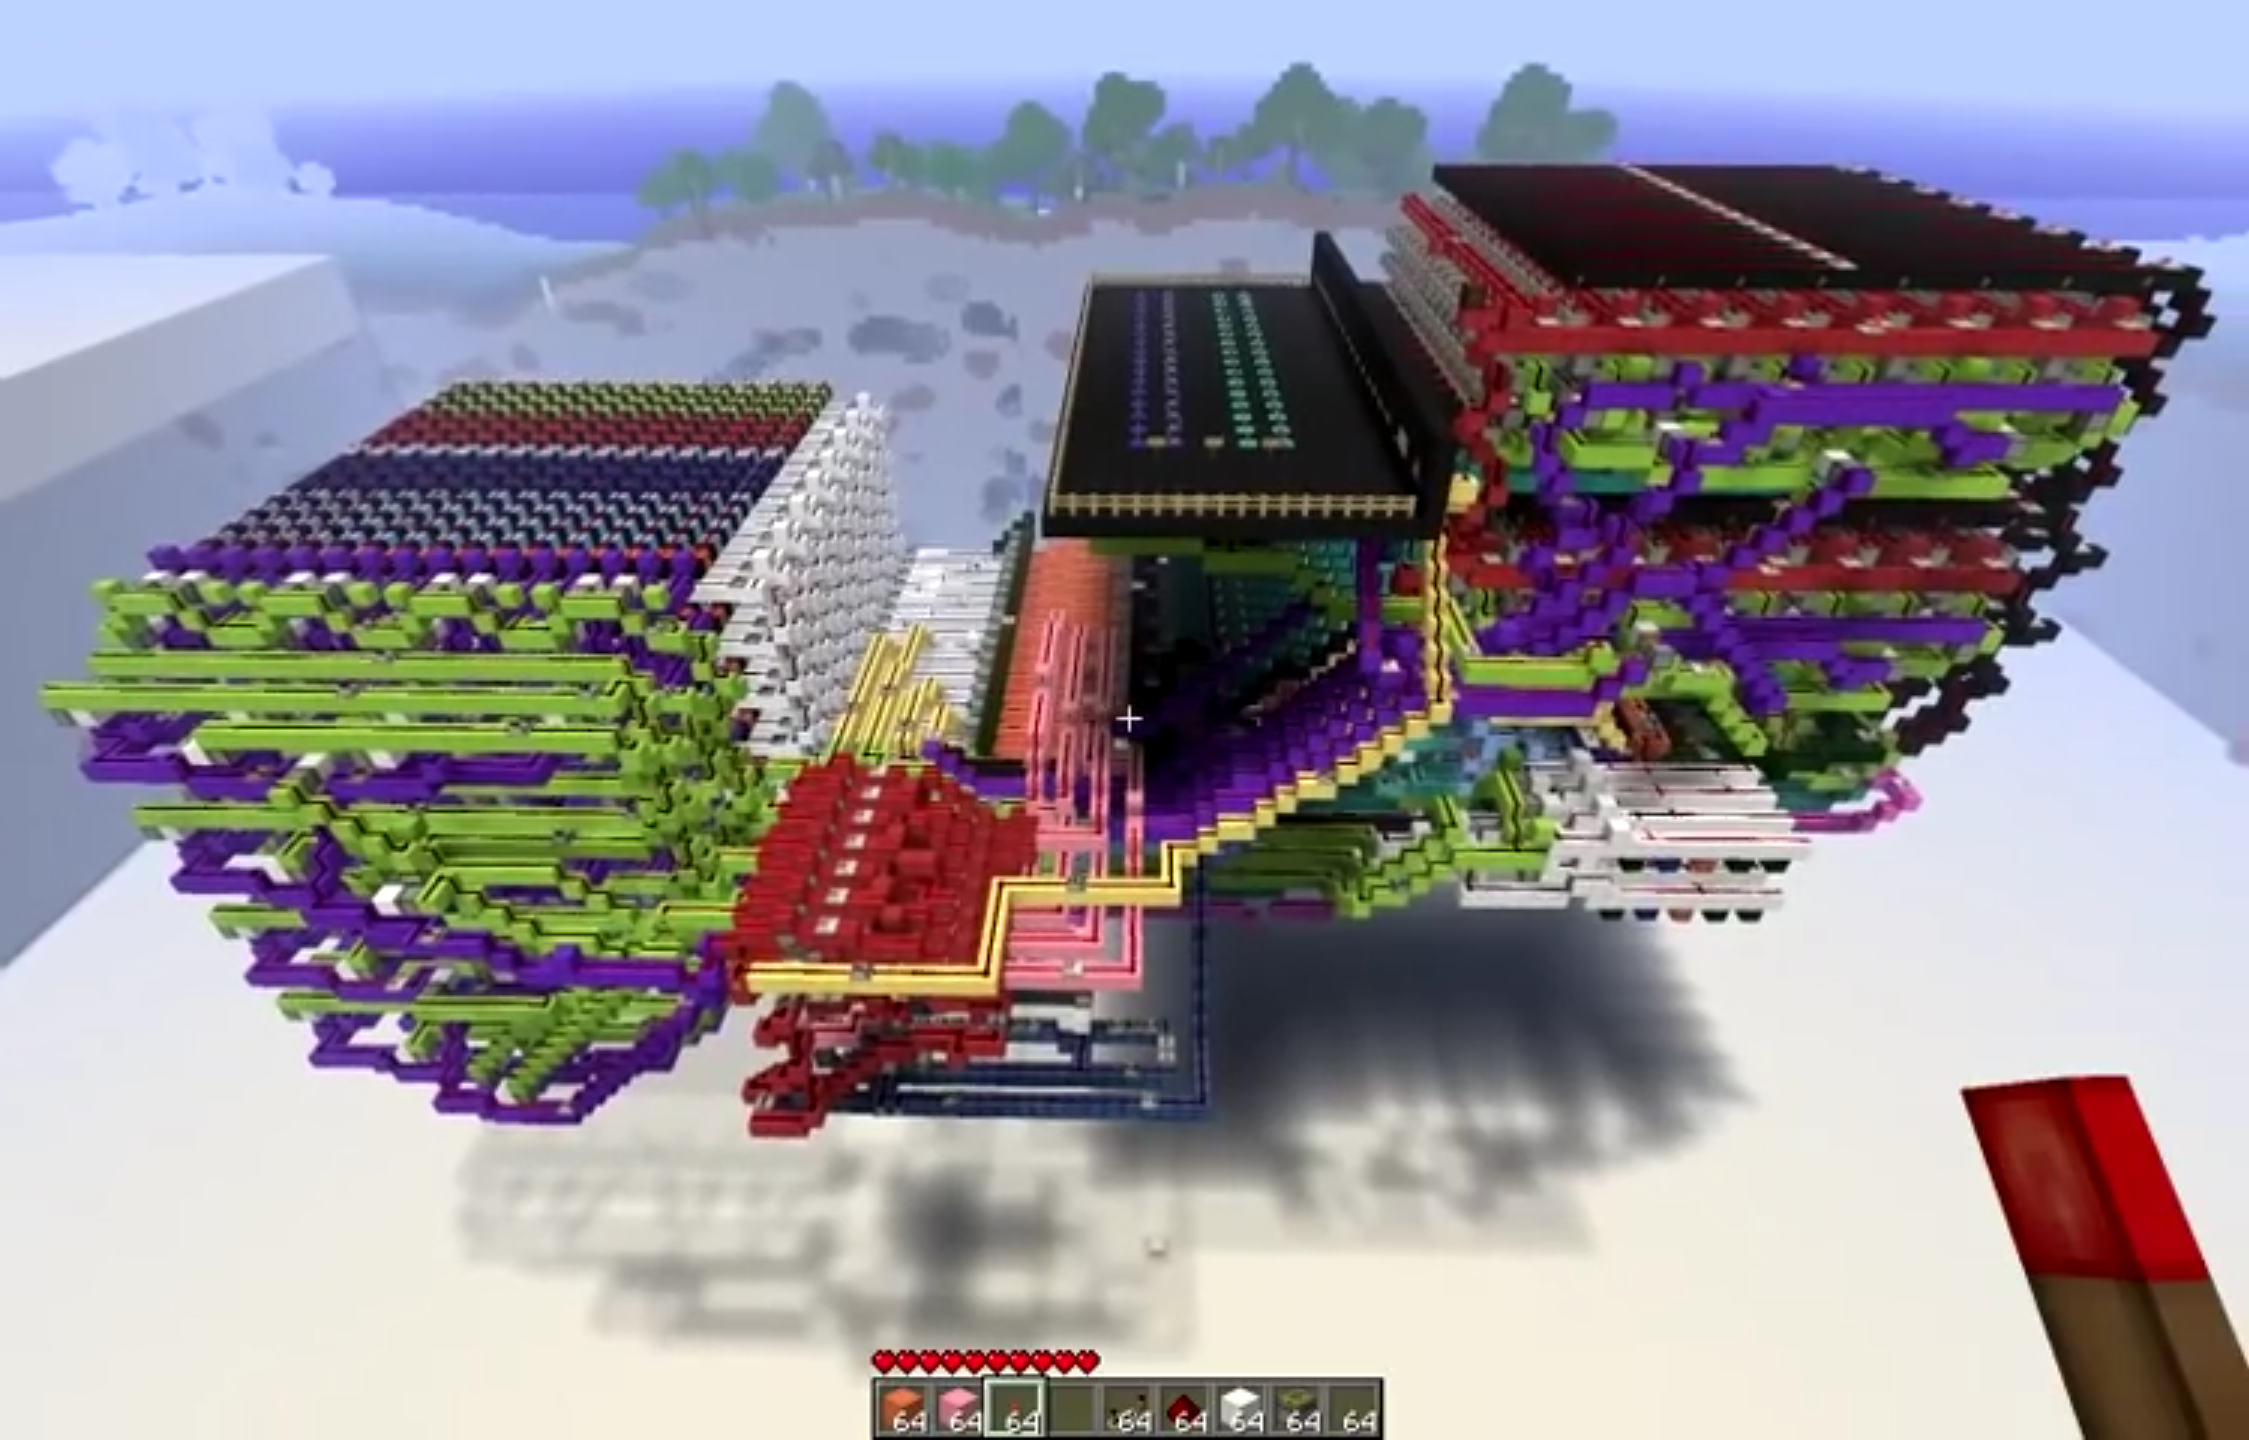
\includegraphics[width=\linewidth]{minecraft.png}
  \caption{Screenshot of a 16 bit computer built in Minecraft by user Ohm.  Full video available on \href{https://www.youtube.com/watch?v=KzrFzkb3A4o}{YouTube}. \textit{Image Credit: Ohm 2011}}
  \label{fig:minecraft}
\end{figure}

The most widely adopted example of discrete design is \href{https://minecraft.net/}{Minecraft}, a PC game that gives players the ability to construct their own worlds from over 100 different block types (Fig \ref{fig:minecraft}).  A subset of these block types form the basis of digital logic in the game and another set of part provide a means of simple 1-bit mechanical actuation \cite{MinecraftWik2016}.  Gameplay and available block types are extendable through various mods and user scripts.
\\

\href{http://golly.sourceforge.net/}{Golly} is a 2D CA simulator originally intended for Conway's game of life, but is extendable to other rulesets.  It implements Gosper's ``hashlife'' algorithm for optimizing the performance of the simulation \cite{Gosper1984}.  Golly's efficient solving and open access has allowed a large online community of CA enthusiasts to collaborate on and experiment with increasingly more complex designs.  In 2013 Dave Greene Wade published the ``Linear Propagator'', a self replicating machine designed in Golly using Conway's ruleset \cite{Greene2013a}.  In 2014, Luke Shaeffer implemented a physically universal CA ruleset in Golly, based on interactions between moving particles \cite{Shaffer2014}.\\

\begin{figure}
  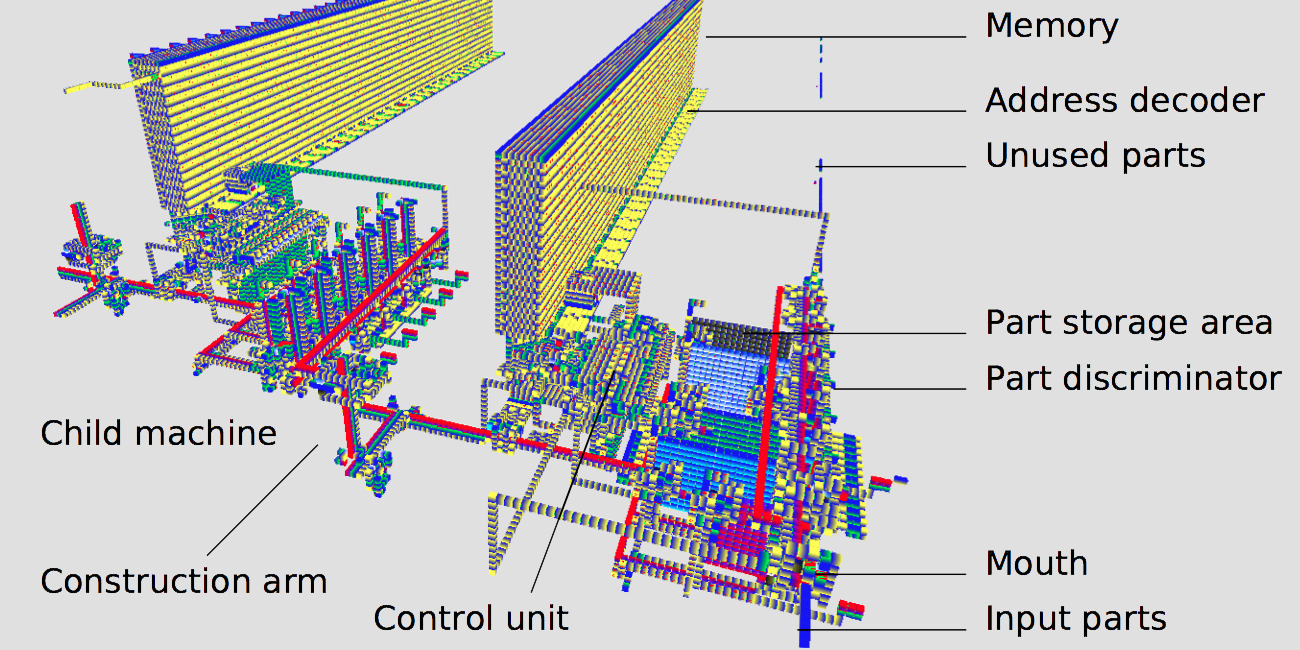
\includegraphics[width=\linewidth]{stevensConstructor.png}
  \caption{A programmable, universal constructor (shown replicating itself) built in CBlock3D by William Stevens from 5040 cells of 6 different types \cite{Stevens2009b}.  Full video of assembly process on  \href{https://www.youtube.com/watch?v=PBXO_6Jn1fs}{YouTube}. \textit{Image Credit: William Stevens 2010}}
  \label{fig:stevensConstructor}
\end{figure}
\href{https://www.youtube.com/watch?feature=player_embedded&v=PBXO_6Jn1fs}{CBlock3D} is a 3D cellular automata environment governed by logical and kinematic rules developed by William Stevens \cite{Stevens2007} \cite{Stevens2009}.  The kinematic simulation in CBlocks3D allows for motions along discrete steps of a regular lattice.  Like Golly, it implements a version of hashlife optimization \cite{Stevens2010} to speed up simulation.  Stevens constructed and simulated a self-replicating machine within this design environment from 5040 cells of 6 distinct types (Fig: \ref{fig:stevensConstructor}) \cite{Stevens2009b}.
\\

\subsection{DNA Origami-Based Tools}

\begin{figure}
  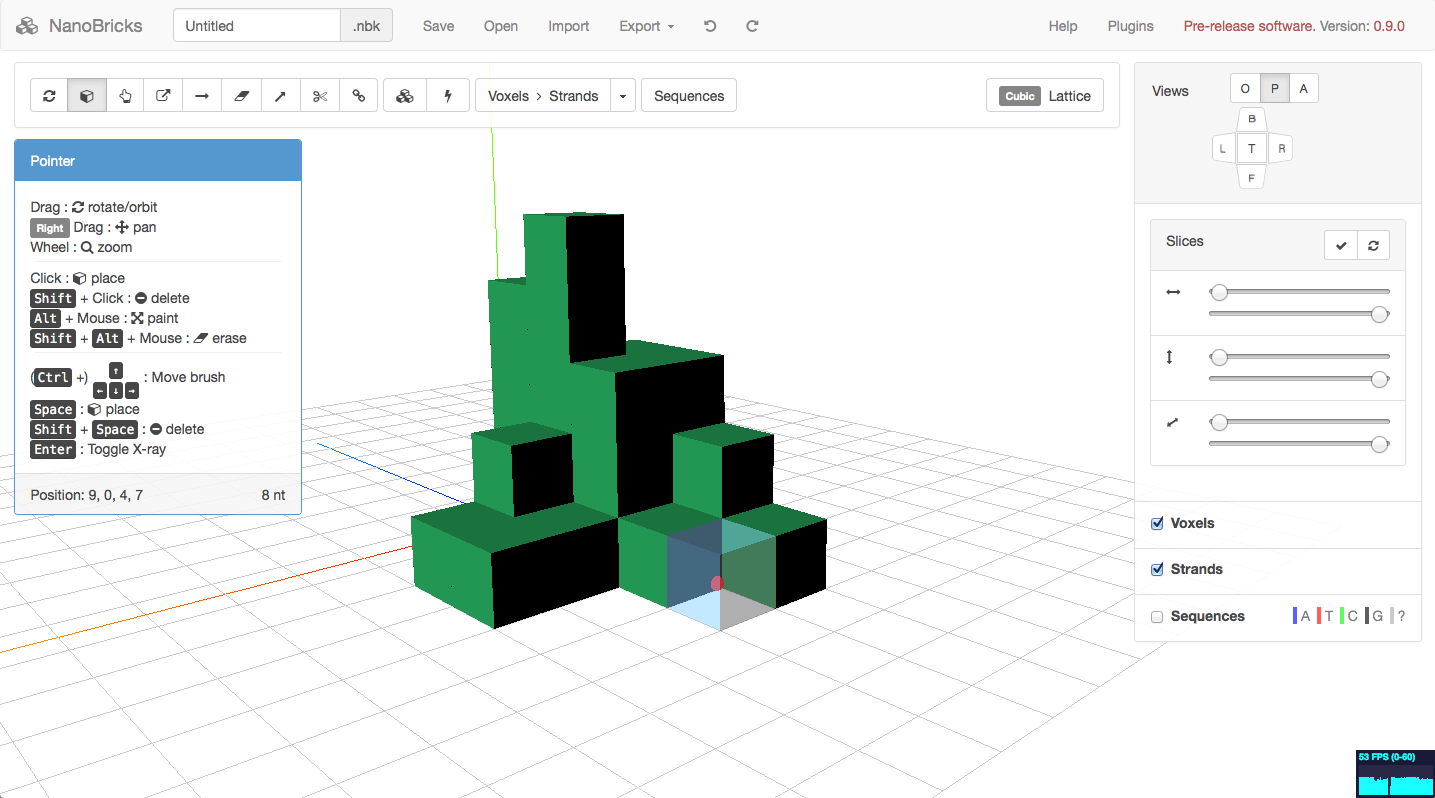
\includegraphics[width=\linewidth]{nanoBricks.png}
  \caption{Screenshot of NanoBricks, a voxel-based design tool for DNA Bricks by the Peng Yin Lab.}
  \label{fig:nanoBricks}
\end{figure}

\href{http://cadnano.org/}{CaDNAno} is a DNA origami design tool originally written by Douglas et al. \cite{Douglas2009}, and later adopted by Autodesk as a plugin for Maya.  It allows users to design 2D and 3D DNA origami structures based on one or several ``scaffold'' strands folded into a particular shape by many ``staple'' strands.  Structures are designed on a regular square or honeycomb lattice, though, single nucleotide insertions and deletions can be added to create programmable, off-lattice bending \cite{Dietz2009} \cite{Kim2012}.\\

\href{http://cando-dna-origami.org/}{Cando} is a DNA origami simulation package developed and maintained by Mark Bathe's group at MIT.  It models double stranded DNA as a homogeneous elastic rod with elastic constants and other physical parameters drawn from empirical measurements \cite{Peters2014}.  Crossovers between double stranded segments are modeled as elastic constraints on the rod elements.  Though these crossovers may deform double stranded segments out of a regular lattice configuration (which they are typically designed in) to form complex 3D geometries, simulated CanDo results show good agreement with experimental results \cite{Kim2012a}.  CanDo supports formats from CaDNAno and other DNA design environments.
\\

\href{http://yin.hms.harvard.edu/bricks/try/}{Nanobricks} is a voxel-based design tool for DNA Bricks.  Nanobricks allows a user to design nano-scale structures with voxels on a cubic lattice; voxel-based designs are converted to sequences and exported as a text file.  Though Nanobricks offers less flexibility than caDNAno (e.g. it does not allow for off-lattice bending designs), it is significantly easier to design valid structures for a novice user.  Direct integration with CanDo is forthcoming.
\\

\subsection{Physics-Based Tools}

\begin{figure}
  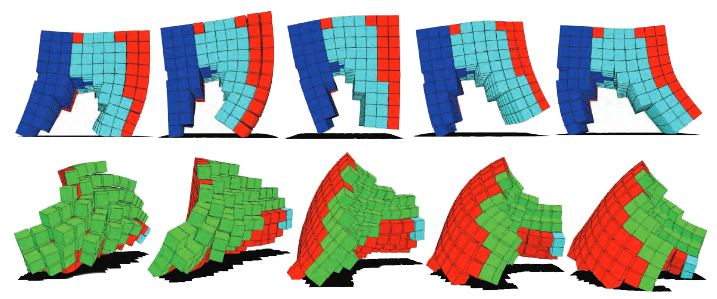
\includegraphics[width=\linewidth]{voxcadWalkers.png}
  \caption{Example gaits of two locomotion robots built from four material types in VoxCAD \cite{Cheney2013b}.  \textit{Image Credit: Cheney et al. 2013}}
  \label{fig:voxcadWalkers}
\end{figure}

\href{http://www.voxcad.com/}{Voxcad} is a physics-based design and dynamic simulation environment by Jonathan Hiller where a user designs virtual soft robots from four block types - two active and two passive \cite{Hiller2014a}.  Though the passive block types descended from a simulation of multimaterial 3D printed voxels, the active block types are not easily fabricated and actuated \cite{Hiller2012} and have not been rigorously evaluated.  Work into the optimization of theoretical locomotion systems in this virtual design space have been explored (Fig: \ref{fig:voxcadWalkers}) \cite{Cheney2013b} \cite{Cheney2013} \cite{Cheney2015}.

}
%%% This is an example first chapter.  You should put chapter/appendix that you
%% write into a separate file, and add a line \include{yourfilename} to
%% main.tex, where `yourfilename.tex' is the name of the chapter/appendix file.
%% You can process specific files by typing their names in at the 
%% \files=
%% prompt when you run the file main.tex through LaTeX.

\singlespacing{


\chapter{Micro Actuators}

supramolecular chemistry


In the sections below, a variety of actuator types are asses based on their performance characteristics.  The scaling laws of each actuator type are derived from the governing physics.

\subsection{Performance Characteristics Definitions}

\textbf{Actuation stress} ($\sigma$) is a measure of the applied force per unit cross-sectional area.  \textbf{Maximum actuation stress} ($\sigma_{max}$) gives the max impulse stress in a stroke of maximum work output.\\

\textbf{Actuation strain} ($\epsilon$) is a measure of the extension/contraction of an actuator relative to its nominal length. \textbf{Maximum actuation strain} ($\epsilon_{max}$) gives the max strain in a stroke of maximum work output.  The \textbf{strain resolution} ($\epsilon_{min}$) is the minimum step in $\epsilon$ possible for a given actuator.\\

\textbf{Actuator density} ($\rho$) gives the ratio of the mass of an actuator to its nominal volume in units of kg/m\textsuperscript{3}.  In this analysis, actuator density is considered independent of the mass of external power supplies, controllers, and fixturing.\\

\textbf{Actuator modulus} ($E$) is the ratio small changes in $\sigma$ to small changes in $\epsilon$ ($d\sigma / d\epsilon$) for a given control signal.\\

\textbf{Maximum actuation frequency} ($f_{max}$) is the max frequency of cyclic operation of a given actuator.  $f_{max}$ may require an external resetting force and may depend on external factors, such as heat dissipation or energy consumption. $f_{max}$ may be so low for some actuators, they should be considered only as single stroke actuators, rather than for cyclic operation.\\

For actuators in sustainable cyclic operation, \textbf{volumetric power} ($p$) is a measure of the mechanical power output per unit volume.\\

\textbf{Efficiency} ($\nu$) is the ratio of mechanical work output to energy input for one complete cycle of operation.\\


\section{Electromagnetic}



\subsection{Solenoid}

\subsection{Voice Coil}

\subsection{Motors}

\subsection{Electro Permanent}

\section{Electrostatic}

%\subsection{Electrostatic Comb Drive}

\section{Piezo}

Piezoelectric materials strain in the presence of an applied electric field $E$.
piezoelectricity $E$
electrostriction $E^{2}$
ferroelectricity (retain at E = 0)

 \begin{equation}\label{eq:diffEq}
\sigma_{max} = E\epsilon_{max}
  \end{equation}
\\
In piezoelectrics, $\epsilon_{max}$ is limited by the material type.  Piezoelectric materials have a maximum tolerable electric field, above which, the material operates in a different regime.
Low strain piezoelectrics: Quartz (SiO\textsubscript{2}), Lithium Niobate (LiNbO\textsubscript{3}), Lithium Tantalate (LiTaO\textsubscript{3})
High strain piezoelectrics: alloys of Lead Zircoate Titanate (PbZr\textsubscript{x}Ti\textsubscript{1-x}O\textsubscript{3}, called PZT)


\section{Shape Memory Alloy}

\section{Magentostrictive}

\section{Thermal}

%\subsection{Wax Actuator}

\section{Pneumatic}

\section{Ultrasonic}

\section{Biological Actuators}


\section{Conclusions}

Further comparison of the performance metrics of mechanical actuators is given in Huber et al \cite{Street1997}.

 is given in Table \ref{tab:actuatorTypes}.

\renewcommand{\arraystretch}{1.5}
%http://tex.stackexchange.com/questions/98388/how-to-make-table-with-rotated-table-headers-in-latex
\begin{table}[h] \label{tab:actuatorTypes}
    \centering
    \caption{Micro-Actuation mechanisms comparison chart.}
\begin{tabular}{ll | *{7}{c} }
    \\
    \multicolumn{2}{c}{Name} 
        & \mcrot{1}{l}{60}{Cost} & \mcrot{1}{l}{60}{Density} & \mcrot{1}{l}{60}{Energy Density} & \mcrot{1}{l}{60}{Efficiency} & \mcrot{1}{l}{60}{Scaling} & \mcrot{1}{l}{60}{Strain} & \mcrot{1}{l}{60}{Etc}\\
    \midrule \midrule

    \multirow{4}{*}{\rotatebox{90}{\textbf{\small{\hspace{17pt}Electromagnetic}}}}
    & Solenoid&
        x & x & x & xxx & x & xxx & -\\
    & Voice-Coil  &
        xx & xxx & xxx & xx & xxx 
        & xx & -\\
    \midrule
    \multirow{4}{*}{\rotatebox{90}{\textbf{\small{\hspace{18pt}Electrostatic}}}}
    & Comb Drive
        & x & x & - & - & x 
        & - & x \\
        
      \midrule
     \multirow{4}{*}{\rotatebox{90}{\textbf{\small{\hspace{14pt}Piezo}}}}
    & PZT
        & x & x & - & - & x 
        & - & x\\
        
        \midrule
     \multirow{4}{*}{\rotatebox{90}{\textbf{\small{\hspace{16pt}Thermal}}}}
    & Paraffin Wax
        & x & x & - & - & x 
        & - & x\\
        
        
                \midrule
     \multirow{4}{*}{\rotatebox{90}{\textbf{\small{\hspace{16pt}Pnuematic}}}}
    & Air-Driven
        & x & x & - & - & x 
        & - & x\\
    & Fluid-Driven 
        & - & - & x & - & - 
        & - & -\\
        
        
    \bottomrule
\end{tabular}
\end{table}


}

%% This is an example first chapter.  You should put chapter/appendix that you
%% write into a separate file, and add a line \include{yourfilename} to
%% main.tex, where `yourfilename.tex' is the name of the chapter/appendix file.
%% You can process specific files by typing their names in at the 
%% \files=
%% prompt when you run the file main.tex through LaTeX.

\singlespacing{

\chapter{Design Hierarchy}

with a scaling factor of about 100x between levels of hierarchy.

The details of the fabrication and joining strategies for these physical parts is beyond the scope of this thesis, though current ideas are briefly addressed here.  Initial thoughts about length scales are included here, but are meant only as a starting point for the 

\section{Elements}

At the lowest level, bulk materials in the form of \textit{elements} are assembled together to form multi-material assemblies.  Our notion of "element" is not an atomic element, but rather a homogenous volume of material with characteristic material properties.  A finite set of elemental types will be chosen based on desirable physical properties, cost, ease of fabrication, and compatibility with other elemental types and assembly processes.\\

For example, an aluminum element type would have the properties of being conductive, stiff, and lightweight and a rubber element type would be insulating and flexible.  Other element types of interest include magnetic and magnetically permeable types, silicon types, actuation types, and thermally conductive and insulating types.\\

Elemental components will be fabricated to a size on the order of ~1-10$\mu$m\textsuperscript{3}.  Some, as yet to be determined, form of joining interface must be incorporated into the geometry of the elemental parts or applied (in the form of an adhesive) to the parts during the assembly process.  This joining strategy may or may not be permanent.

\section{Functions}

Assemblies of elements form \textit{functions} - larger scale part types with material properties defined by their constituent elements.  As the name suggests, functions are categorized based on higher-level interactions with neighboring electro-mechanical systems, rather than their bulk material properties.  Function-level components fall into one of several functional archetypes, including but not limited to n-degree-of-freedom mechanical latches, hinges, and actuators, electronic memory storage, electronic oscillators, timers, and programmable logic.  Anisotropic patterns of elemental types within a function-level component may give the function tunable anisotropic behaviors.\\

Examples of function-level components would be routing components, which pass one or several electronic signals to neighboring components, or a one degree-of-freedom hinge, which displays low bending stiffness around one axis and high stiffness in the remaining directions.  This level of design hierarchy would grow to include actuators with tunable anisotropy, strain, and stress, and simple programmable silicon parts.  A more complete discussion of the diversity of mechanical part types at the function-level is given in Chapter \ref{chap:functionSim}.\\

Functional components will be on the order of ~1mm\textsuperscript{3}.  Some form of common interface must allow for both mechanical loads and analog electronic signals to pass from one function component to another.  At the function-level, a reversible joining interface is preferred so that reconfigurable behavior and recycling is possible.

\section{Modules}

\textit{Modules} are assemblies of function-level components, joined together to form robotic subsystems.  Modules combine electronic and mechanical functionality to achieve singular, high-level robotic tasks.  Modules will communicate with each other through an abstracted, digital interface.  Each module will own its own microprocessing unit that coordinates its function-level actuators and other active components.  This way, the low-level description of the structure within a module remains internal to the module itself.\\

Examples of modules include end effectors like grippers, clamping mechanisms, and sensors, actuation/locomotion systems, energy storage and generation, and large memory or programmable logic banks.  Joining interfaces between modules will allow mechanical forces, power, and a few digital signals to pass from one module to the next.  As with functions, modules should be reversibly joined.  The interface between modules may consist of many parallel function-level interfaces, or a bulk, module-level interface.\\

Modules will be built on the order of ~1cm\textsuperscript{3}.  Though modules may use mechanical compliance at the function-level to increase their internal degrees of freedom, at larger scales modules act as rigid bodies with internal motion.  That is, internal mechanical compliance within a module does not propagate to interactions with neighboring modules.  This idea follows from a model of how traditional solid-bodied rotary and linear actuators are viewed within a larger robotic structure.

\section{Complexes}

Assemblies of modules form \textit{complexes}, self-contained robotic systems that coordinate their own sensing, memory, logic, power, and/or actuation.  The key distinction between the module and complex-level is that complexes integrate inputs, outputs, logic, and memory, whereas modules specialize in only one of these tasks.  A complex could be a single, locomoting robot or manipulator, or an active, environmental system that performs sensing, actuation, or logical tasks across space.\\

Complexes will interact with function-level and module-level feedstock to accomplish assembly tasks.  shuttles materials across it (like a conveyor belt)\\

Complexes will be comprised of several to hundreds of individual modules, spanning length scales on the order of ten of cm to m.  Complexes should be considered independent, self-contained units.  The interface between complexes will be governed by end effector modules that the complex owns.

\section{Systems of Complexes}

Many complexes of various forms and functions may work together at a \textit{system}-level to accomplish large scale tasks.  More layers of hierarchy could be developed across this 

\section{Design Hierarchy in Biology}

\begin{sidewaysfigure}
  \includegraphics[width=\textwidth,height=\textheight,keepaspectratio]{ProteinHierarchy.png}
  \caption{Hierarchical breakdown of protein complexes (complexes) into proteins (modules), amino acids (functions), and atoms (elements).}
  \label{fig:ProteinHierarchy}
\end{sidewaysfigure}


Currently, the only known example of a physical, self-replicating system is the biology that has evolved on Earth.  Though we observe some slight variation across species, all biological self replication involves the use of protein machinery (called "protein complexes") built primarily from a small set of amino acid building blocks.\\

The construction of protein complexes takes place in a hierarchical fashion.  Figure \ref{fig:ProteinHierarchy} describes the hierarchical breakdown of protein complexes in terms of the four levels of hierarchy established earlier in this chapter; protein complexes (complex-level objects) are decomposed into proteins (modules), then into amino acids (functions), and finally into atomic elements (elements).  This hierarchical breakdown is slightly different from the primary/secondary/tertiary/quaternary structures typically used to discuss the levels of protein description.  The similarity of some of the biological nomenclature to our own hierarchical nomenclature is due to the fact that it was derived from the biological model.

\subsection{Elements, Functional Groups, and Functions}

At the most fundamental level, biological structures are composed of atoms of various elemental types.  Most biological molecules on Earth, especially those involved in protein synthesis and activation, are made from combinations of carbon, hydrogen, nitrogen, oxygen, phosphorus, and sulfur (CHNOPS).\\

Each element's unique position on the periodic table dictates its physical properties, which have implications in higher-level structures formed from the elements.  These properties include the element's mass, the number of covalent bonds it can form, the number of paired electrons it contains in its outermost electron shell, the polarization of the bonds and molecules it forms with other elements, and the stability of its bonds in various environments.\\

Certain motifs of covalently bonded atoms form \textit{functional groups} within molecules.  Functional groups determine the ability of a molecule to undergo various archetypal reactions (addition, substitution, elimination, etc) functional groups on other molecules.  A subset of the important functional groups found in biochemistry are indicated in Figure \ref{fig:ProteinHierarchy}.  "R" indicates an arbitrary side-chain, where the functional group connects to the rest of the molecule.\\

%In organic chemistry, the identification of functional groups allow us to abstract the interactions between molecules based on to predict how they will react in certain conditions.


\begin{figure}
  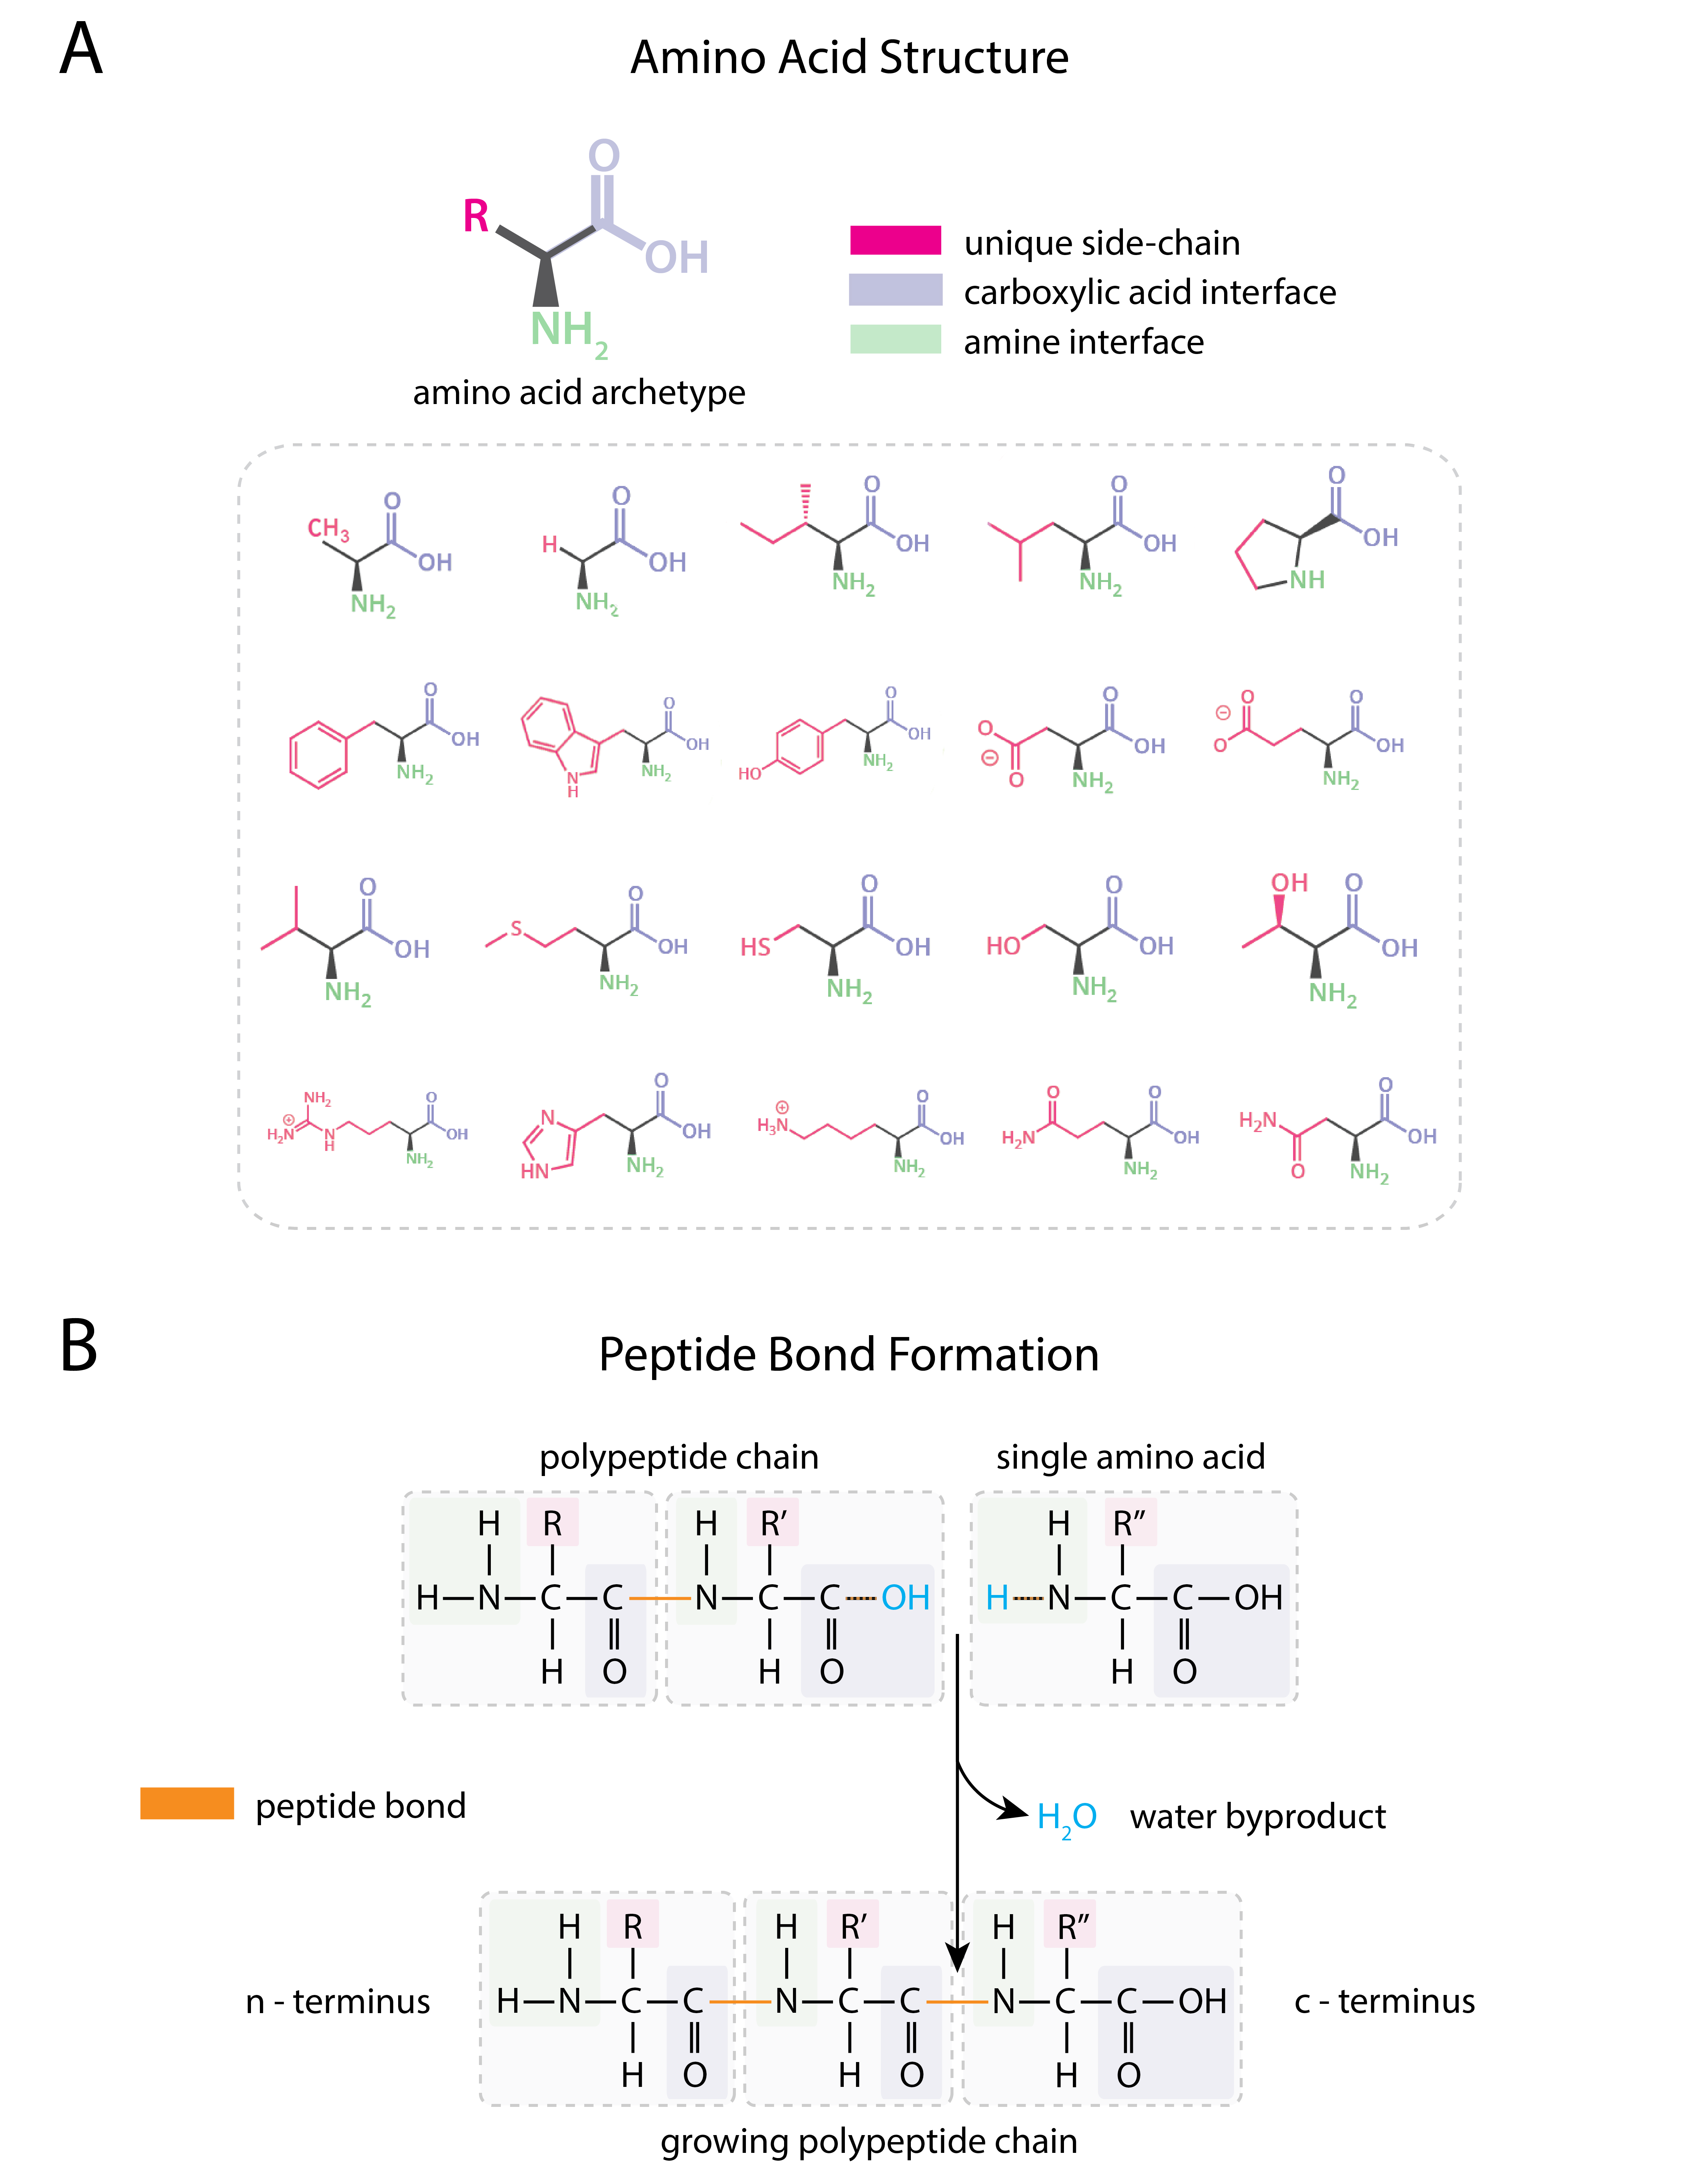
\includegraphics[width=\textwidth]{AminosInterface.png}
  \caption{(A) Decomposition of amino acids into carboxylic acid and amine interfaces and unique side-chain. (B) Formation of peptide bond at c-terminus (carboxylic acid group) of polypeptide chain with the n-terminus (amine group) of an amino acid. One molecule of water is produced as a byproduct of the peptide bonding reaction.  R, R', and R'' represent arbitrary amino acid side-chains.  Peptide bonds bolded.}
  \label{fig:AminosInterface}
\end{figure}

\textit{Amino acids} are molecules which contain several functional groups.  As indicated in Figure \ref{fig:AminosInterface}A all amino acids contain a carboxylic acid (COOH) and an amine group (NH\textsubscript{2} or NRH).  The purpose of these groups is to form the peptide bonds between amino acids in a polypeptide chain.  Peptide bonding forms a covalent bond between two amino acids through a process called "condensation", with a single molecule of water created as a byproduct \ref{fig:AminosInterface}B.\\

The remaining portion of an amino acid molecule (indicated by "R" in the amino acid archetype in Figure \ref{fig:AminosInterface}A, we'll call it "\textit{the} side-chain") determines its unique properties specific to each type of amino acid.  This side-chain may consist of one or more distinct functional groups.  Amino acids are characterized according to their side-chains in several ways; one grouping is shown in Figure \ref{fig:ProteinHierarchy}, with amino acids described by size, polarity, nucleophilicity, the presence of aromatic rings, acidity or basicity, and the presence of amide groups.\\

We can think of each of the amino acids as being composed of a standard interface and a unique, functional side-chain in the same way that our function-level engineered parts will be comprised of a standard interface and a unique, functional interior.  The carboxylic and amine groups common to all amino acids allow for polymerization along one dimension, and subsequent folding into three dimensions; we plan to design our interface to accommodate something analogous to "polymerization" in three dimensions.\\

 \subsection{Modules and Complexes}

Polypeptide chains typically consisting of hundreds of amino acids fold to form three dimensional \textit{proteins}.  

\subsection{Systems}

Beyond protein complexes, more levels of hierarchy exist within biological organisms to carry out systems-level tasks.  Protein complexes can be grouped according to the chemical pathways they interact with within a cell, by the organelles they belong to                                                                                                                                                                                                 

Organelles are organized within cells, cells within tissues, tissues within organs, organs within even higher level systems, and ultimately these systems come together in one complete organism.

\subsection{Scaling}

In the biological example, each level of hierarchy introduces a factor of about 10x in scaling.  The atoms that compose the lowest level of hierarchy have covalent diameters ranging from 50-200pm \cite{Slater1993}.  Amino acid diameters can be roughly calculated from atomic radii and three-dimensional structure to a range of 0.42-1.2nm \cite{Pool2003}.  The average protein length across prokaryotes and eukaryotes is about 200-400 amino acids, with a mass of about 20-40kDa \cite{Brocchieri2005}.  Assuming a simple spherical shape, this mass translates to a typical protein diameter of about 3-4nm \cite{Erickson2009}.  Known protein complexes are comprised of two to several hundred protein monomers with typical complex diameters ranging from about 8-100nm \cite{Yang2010a}.\\

Beyond these first four hierarchical levels, higher systems...
Assembly within is not carried out by a single protein complex, but rather, by the coordinated efforts of several complexes.

\subsection{Combinatorial Space}

number of elements\\
number of amino acids - ribozyme, other species\\
number of protiens\\
number of complexes - design modularity\\

\subsection{Fabrication}

synthesis of amino acids? recycling, breakdown to function level

\section{Design Hierarchy in Conway's Game of Life}

In the 1940's Von Neumann began studying the requirements for self-replication and evolvability in artificial, CA worlds \cite{Neumann1966}.  One such world that has gained widespread notoriety is Conway's Game of Life ("Life").  Since it's inception in 1970, Life has developed a cult following of researchers, engineers, and hobbyists, pushing each other to construct increasingly elaborate "machines" from pixels on a screen.  These investigations have resulted in a lengthy taxonomy of motifs, reactions, mechanisms, and complex engineered systems within Life.  Some notable accomplishments include Gemini (an oblique spaceship encoded by a long glider tape)\cite{Wade2010}, the Linear Propagator (a self replicating machine)\cite{Greene2013}, a Universal Turing Machine \cite{Rendell2000}, and the OTCA Metapixel (a structure that behaves like a large-scale Life pixel)\cite{Due2006}.\\

The analogies between machines in Life and our proposed assembly system are limited, due to the fact that Life is inherently non-physical; it violates basic conservation principals, has no notion of cell joining, and is based on highly abstracted interactions.  However it provides an example of how engineered self-replication is possible using extremely simple building blocks, so-called "non-trivial" self-replication.  A proof of the existence of non-trivial self-replicating patterns in Life was first published by Conway, Berekamp, and Guy in 1982\cite{Berekamp1982}, and several decades later the first implementations of non-trivial replicators began emerging on online Life forums.  This work argues that the basic requirements for self-replication - universal computation and universal construction - are not only \textit{not} unique to biology, but are, in fact, quite prevalent in other virtual and physical systems.  An excellent analysis of Conway's existence proof, as well as an introduction to important concepts in Life can be found in \textit{The Recursive Universe} by William Poundstone\cite{Poundstone1985}.\\

\begin{figure}
  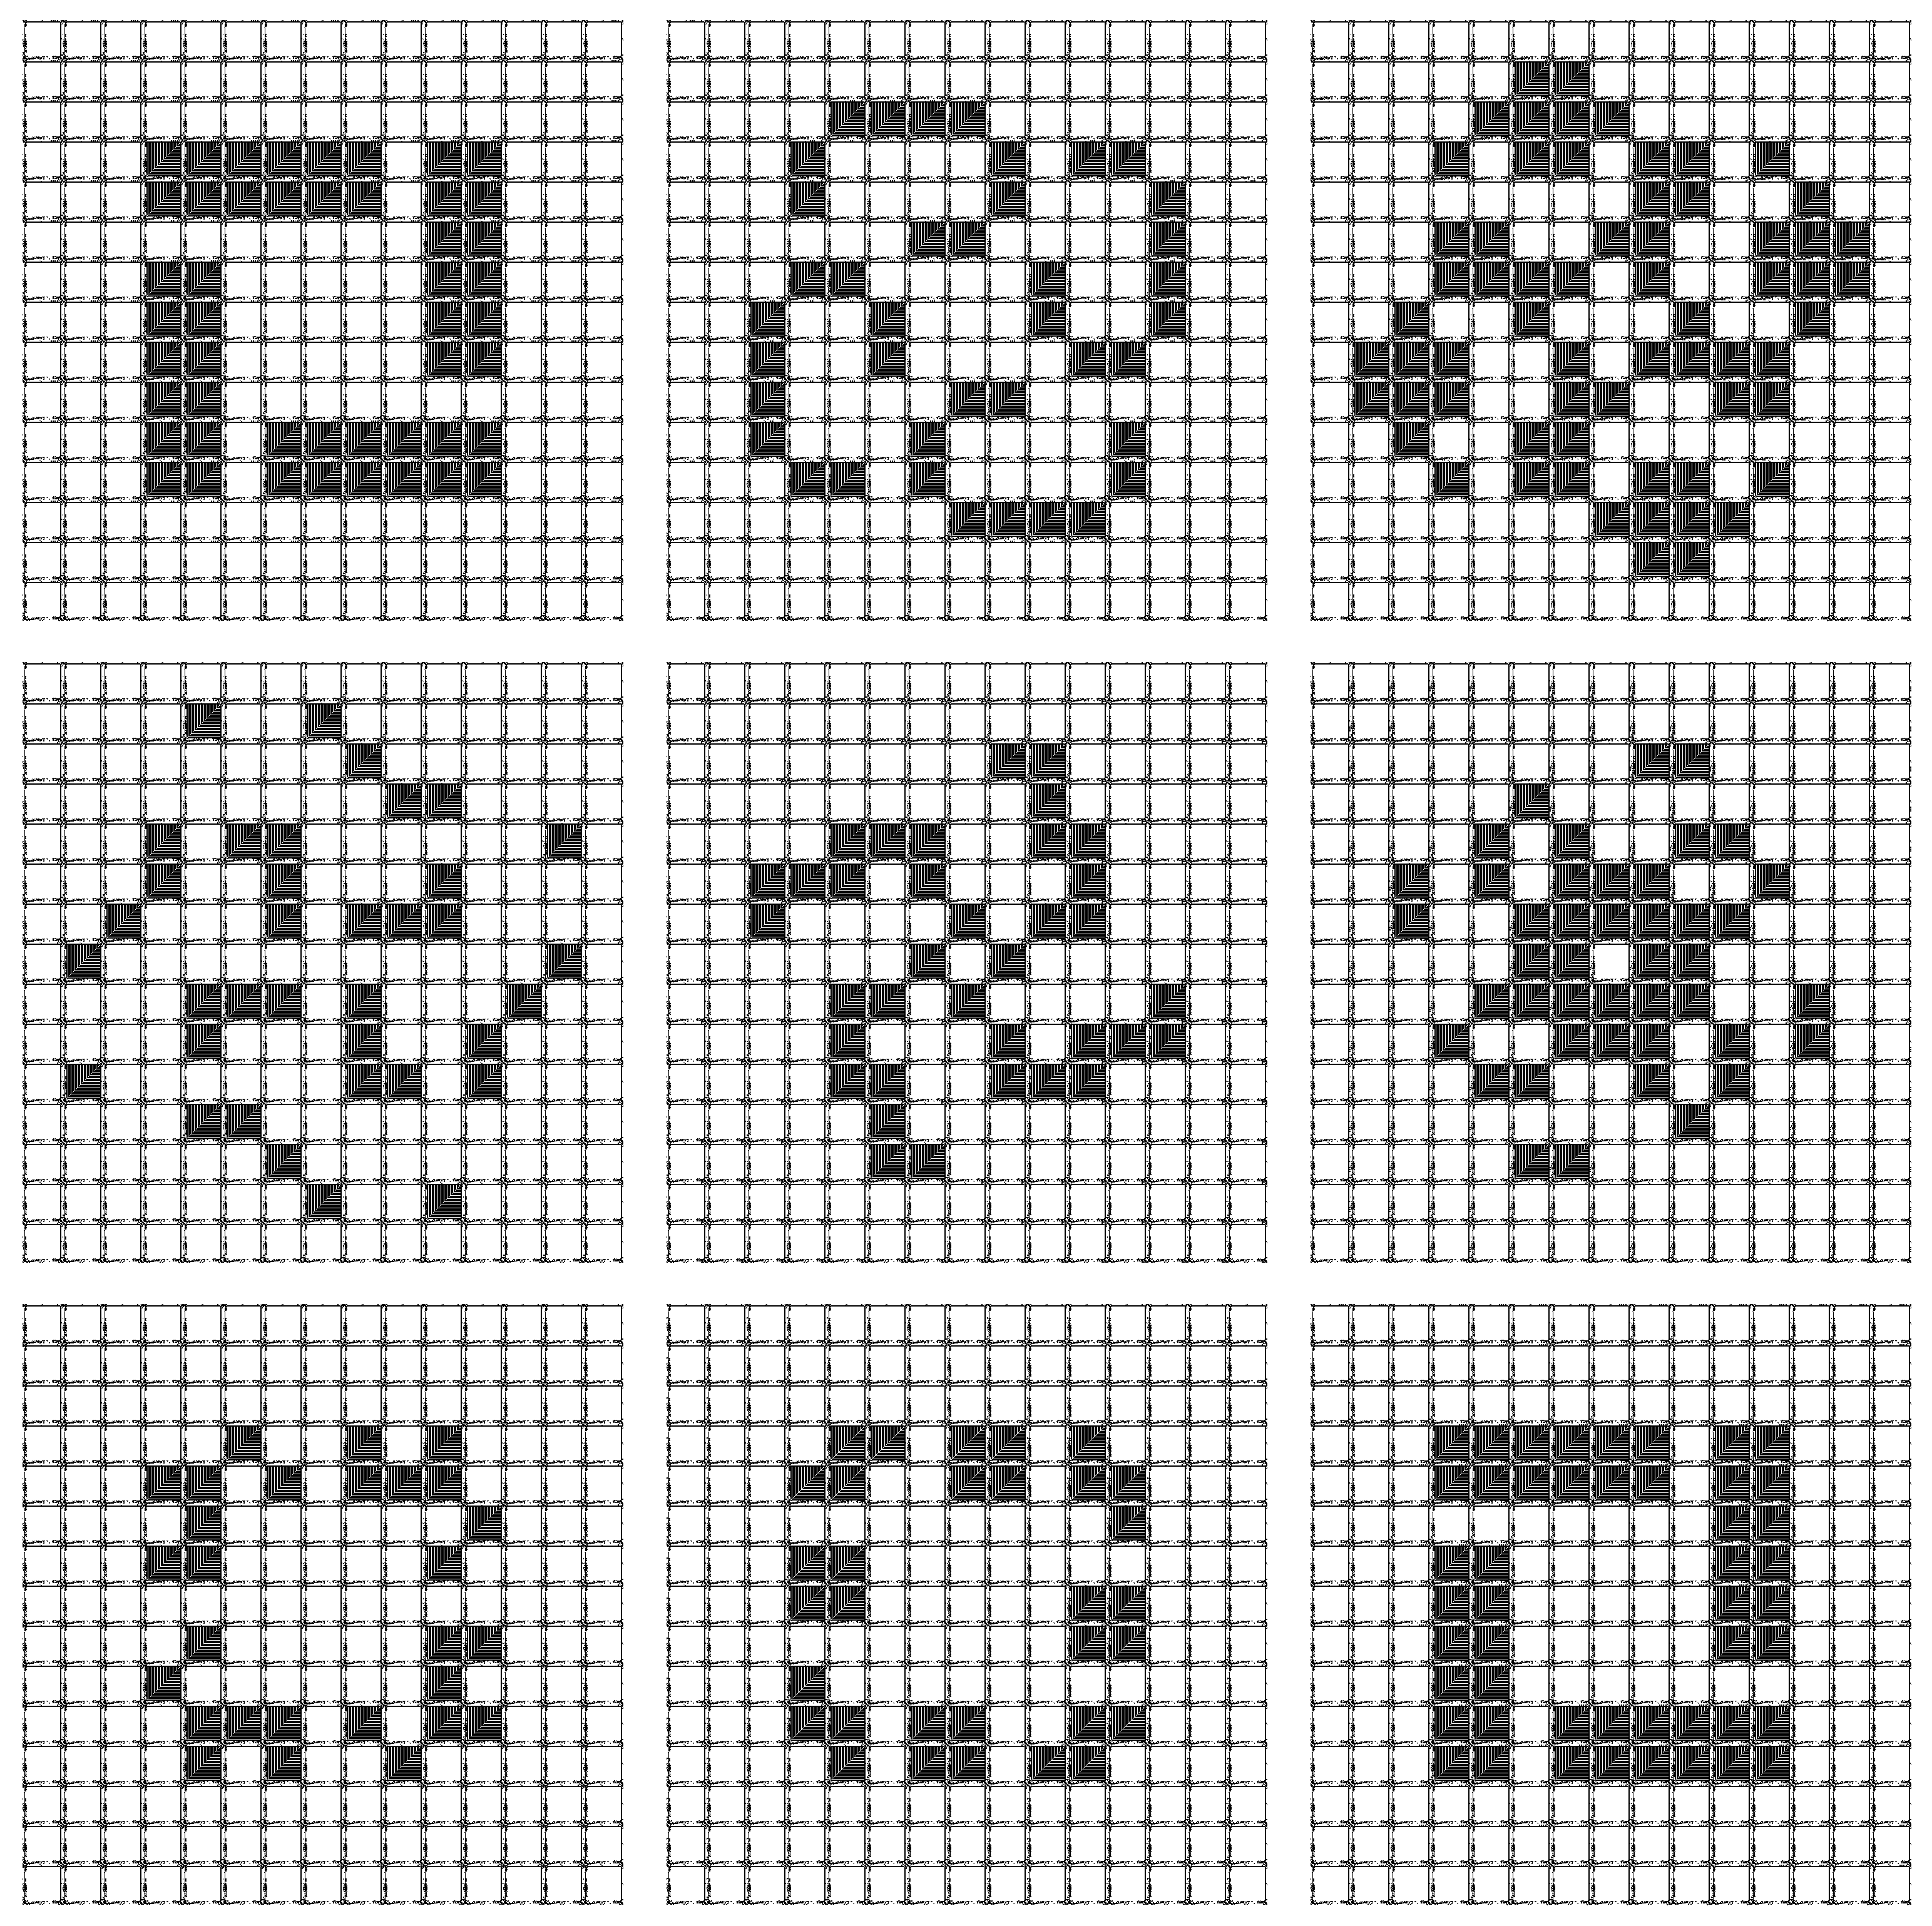
\includegraphics[width=\textwidth]{OTCAGalaxy.png}
  \caption{Nine timesteps of a 15x15 array of OTCA Metapixels playing out a period-8 oscillating pattern called Kok's Galaxy.  Each timestep represents 35,328 generations of Life for a total of 282,624 generations for the entire repeating sequence.  Each metacell occupies 2058x2058 Life cells, for a total of 30,800x30,800 Life cells for the whole 15x15 metacell array (this accounts for a 5 cell overlap between adjacent metacells).}
  \label{fig:OTCAGalaxy}
\end{figure}

In the next sections, I'll analyze a particularly complex Life pattern in terms of the hierarchies I introduced earlier in the chapter.  The OTCA Metapixel was designed by Brice Due in 2006\cite{Due2006}\cite{Ghassaei2015}.  Though not the first \textit{metacell} (a structure that can mimick a CA cell), it is the first \textit{metapixel} (a structure that looks and behaves like a macro-scale CA pixel) built in Life, and it can be programmed to perform any CA ruleset that's based on a summation of a cell's 8 local neighbors.  Many metapixels can be patterned together on a grid to play out a macro-scale CA (Figure \ref{fig:OTCAGalaxy}).

\subsection{Elements, Motifs, and Functions}

The first few levels of hierarchy within Life are illustrated in Figure \ref{fig:OTCAMetaHierarchy}.  At the most basic level, structures within Life are constructed from \textit{cells}.  Cells are represented by one pixel on a Life grid and store a binary state - "living" or "dead".\\

Small assemblies of cells form \textit{motifs} on the order of about 5 cells across.  \textit{Still Lifes} are a category of motif that are static across generations unless acted upon by another pattern.  \textit{Oscillators} morph between several conformations at some regular time interval.  Oscillators are categorized based on their periodicity, for example, the Blinker and Beacon (Figure \ref{fig:OTCAMetaHierarchy}) are period-2 oscillators, and Kok's Galaxy (Figure \ref{fig:OTCAGalaxy}) is a period-8 oscillator.  \textit{Spaceships} are oscillators that move across the Life grid as they oscillate.  Gliders are the smallest type of spaceship, they move across space in diagonal directions.  Other spaceships, like Light Weight, Medium Weight or Heavy Weight Spaceships (LWSS, MWSS, and HWSS, respectively) move in cartesian directions.  Spaceships are categorized based on their periodicity and on their speed.  \textit{Methuselahs} are small patterns that take a large number of generations to eventually stabilize.  R-Pentamino is a Methuselah of only 5 initial cells that stabilizes in 1103 generations.\\

At the function-level, Life patterns on the scale of about 50 cells

\begin{sidewaysfigure}
  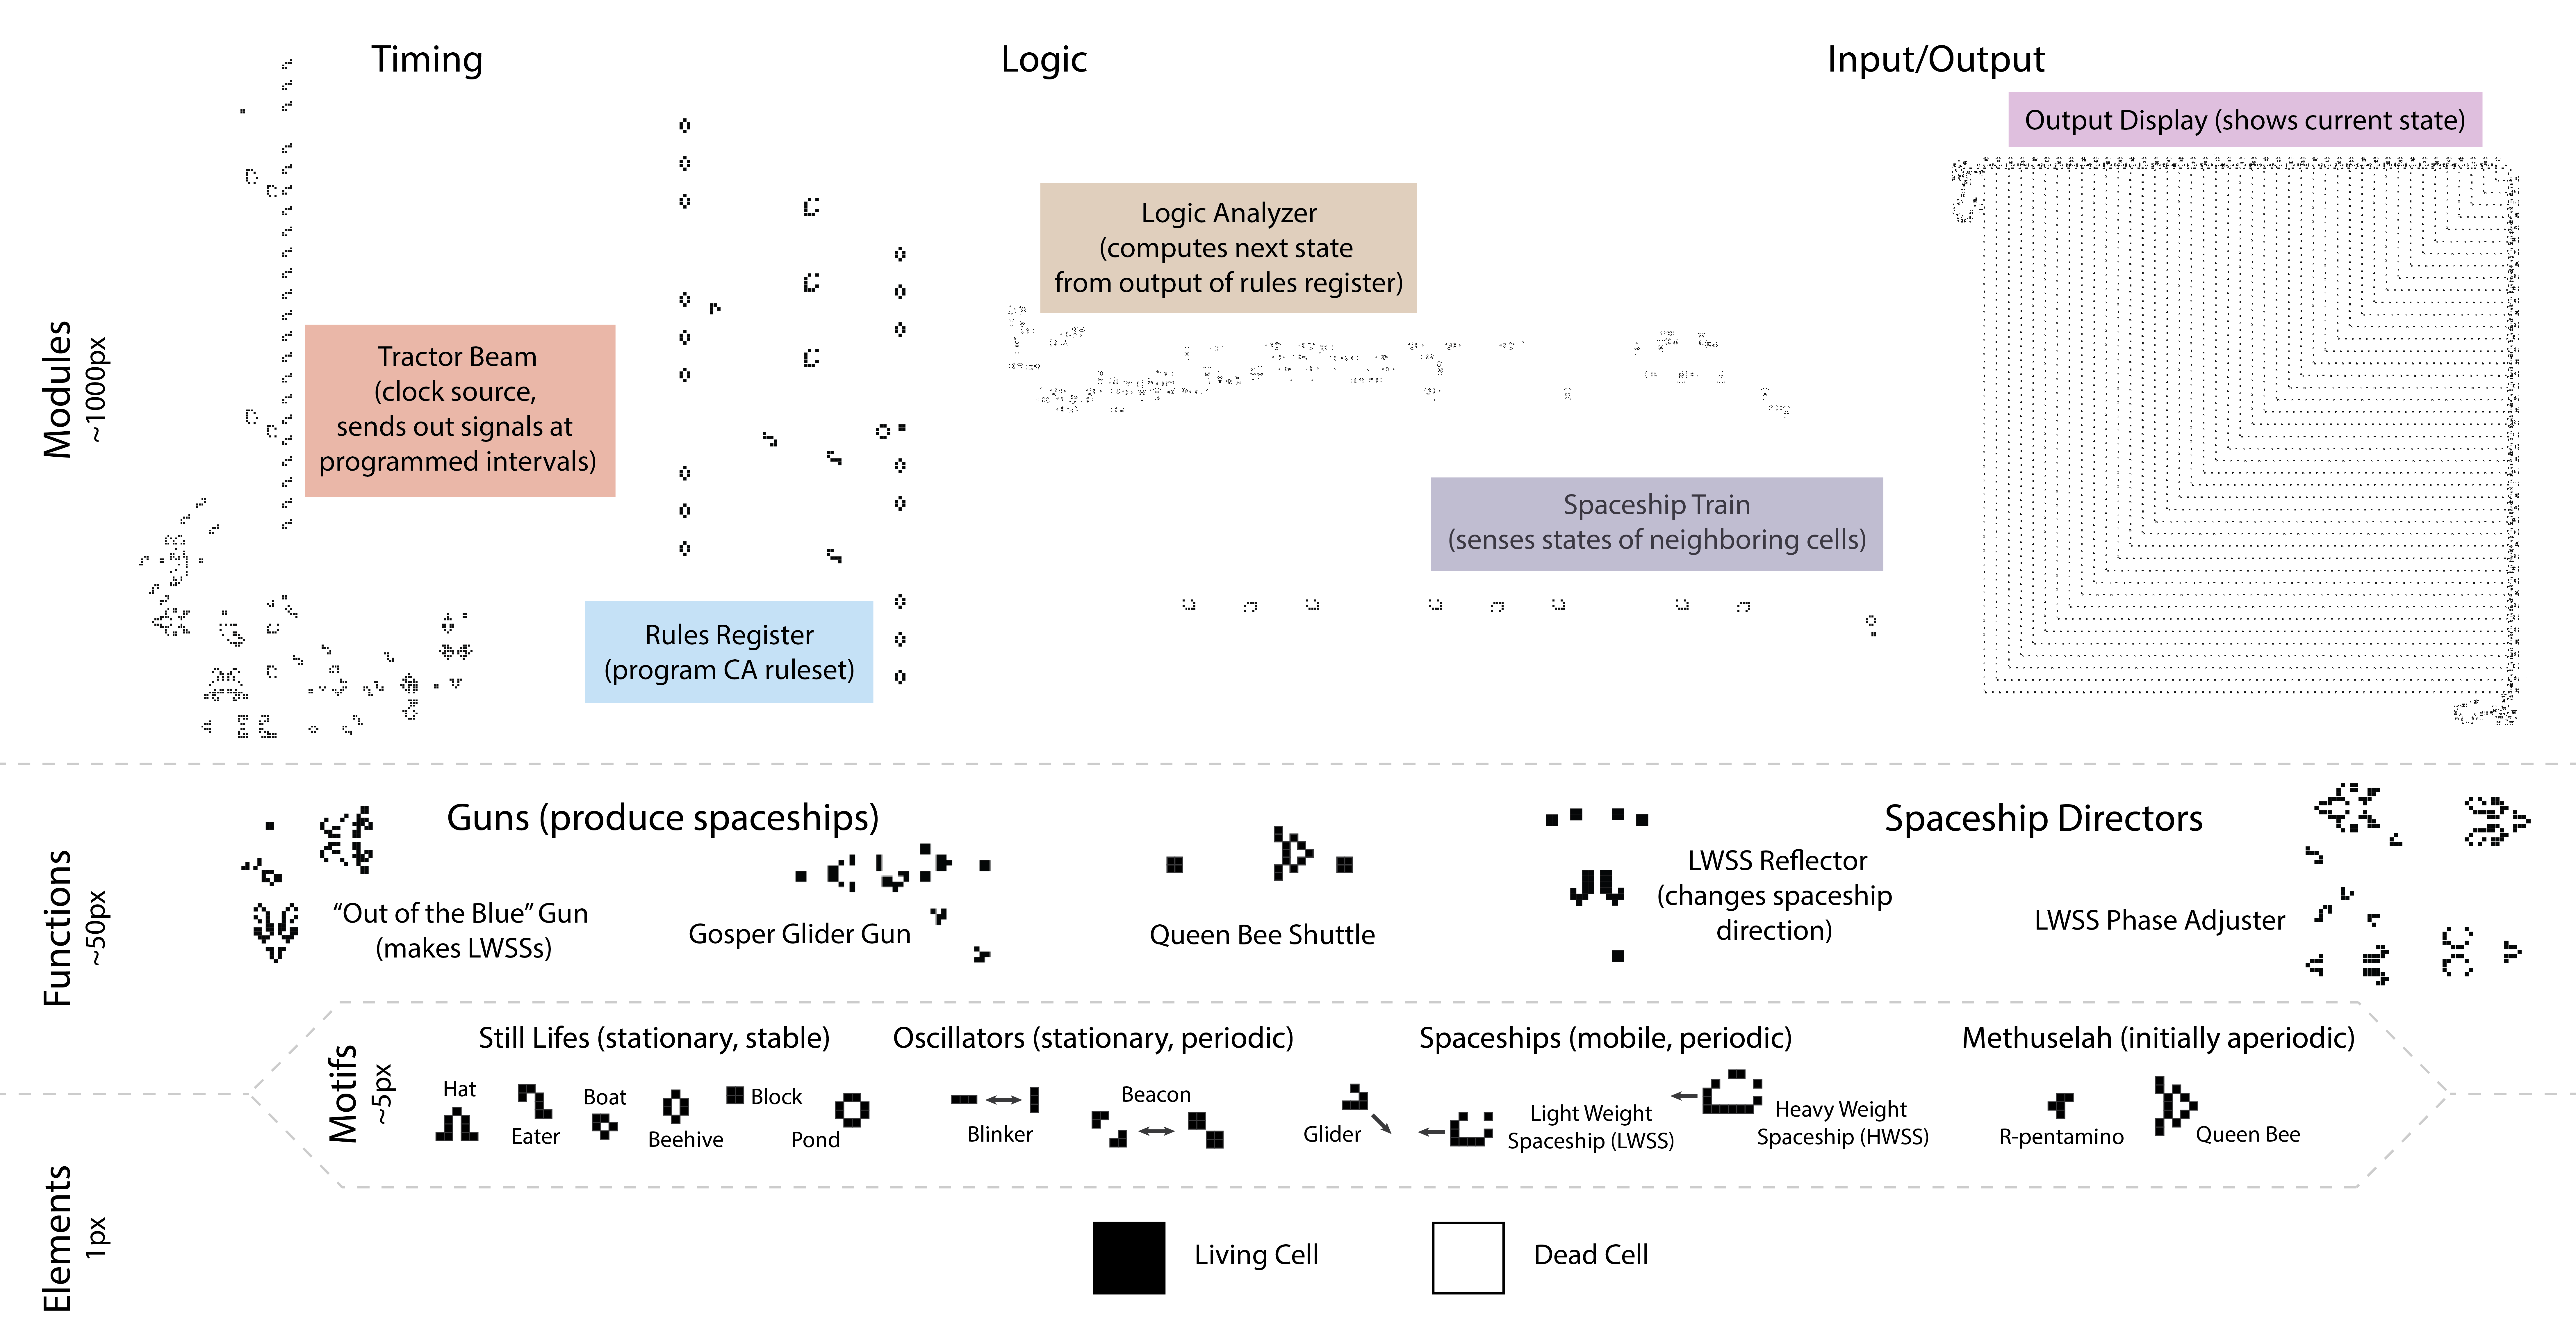
\includegraphics[width=\textwidth,height=\textheight,keepaspectratio]{OTCAMetaHierarchy.png}
  \caption{Hierarchical breakdown of OTCA Metapixel.}
  \label{fig:OTCAMetaHierarchy}
\end{sidewaysfigure}

\subsection{Modules and Complexes}

\begin{figure}
  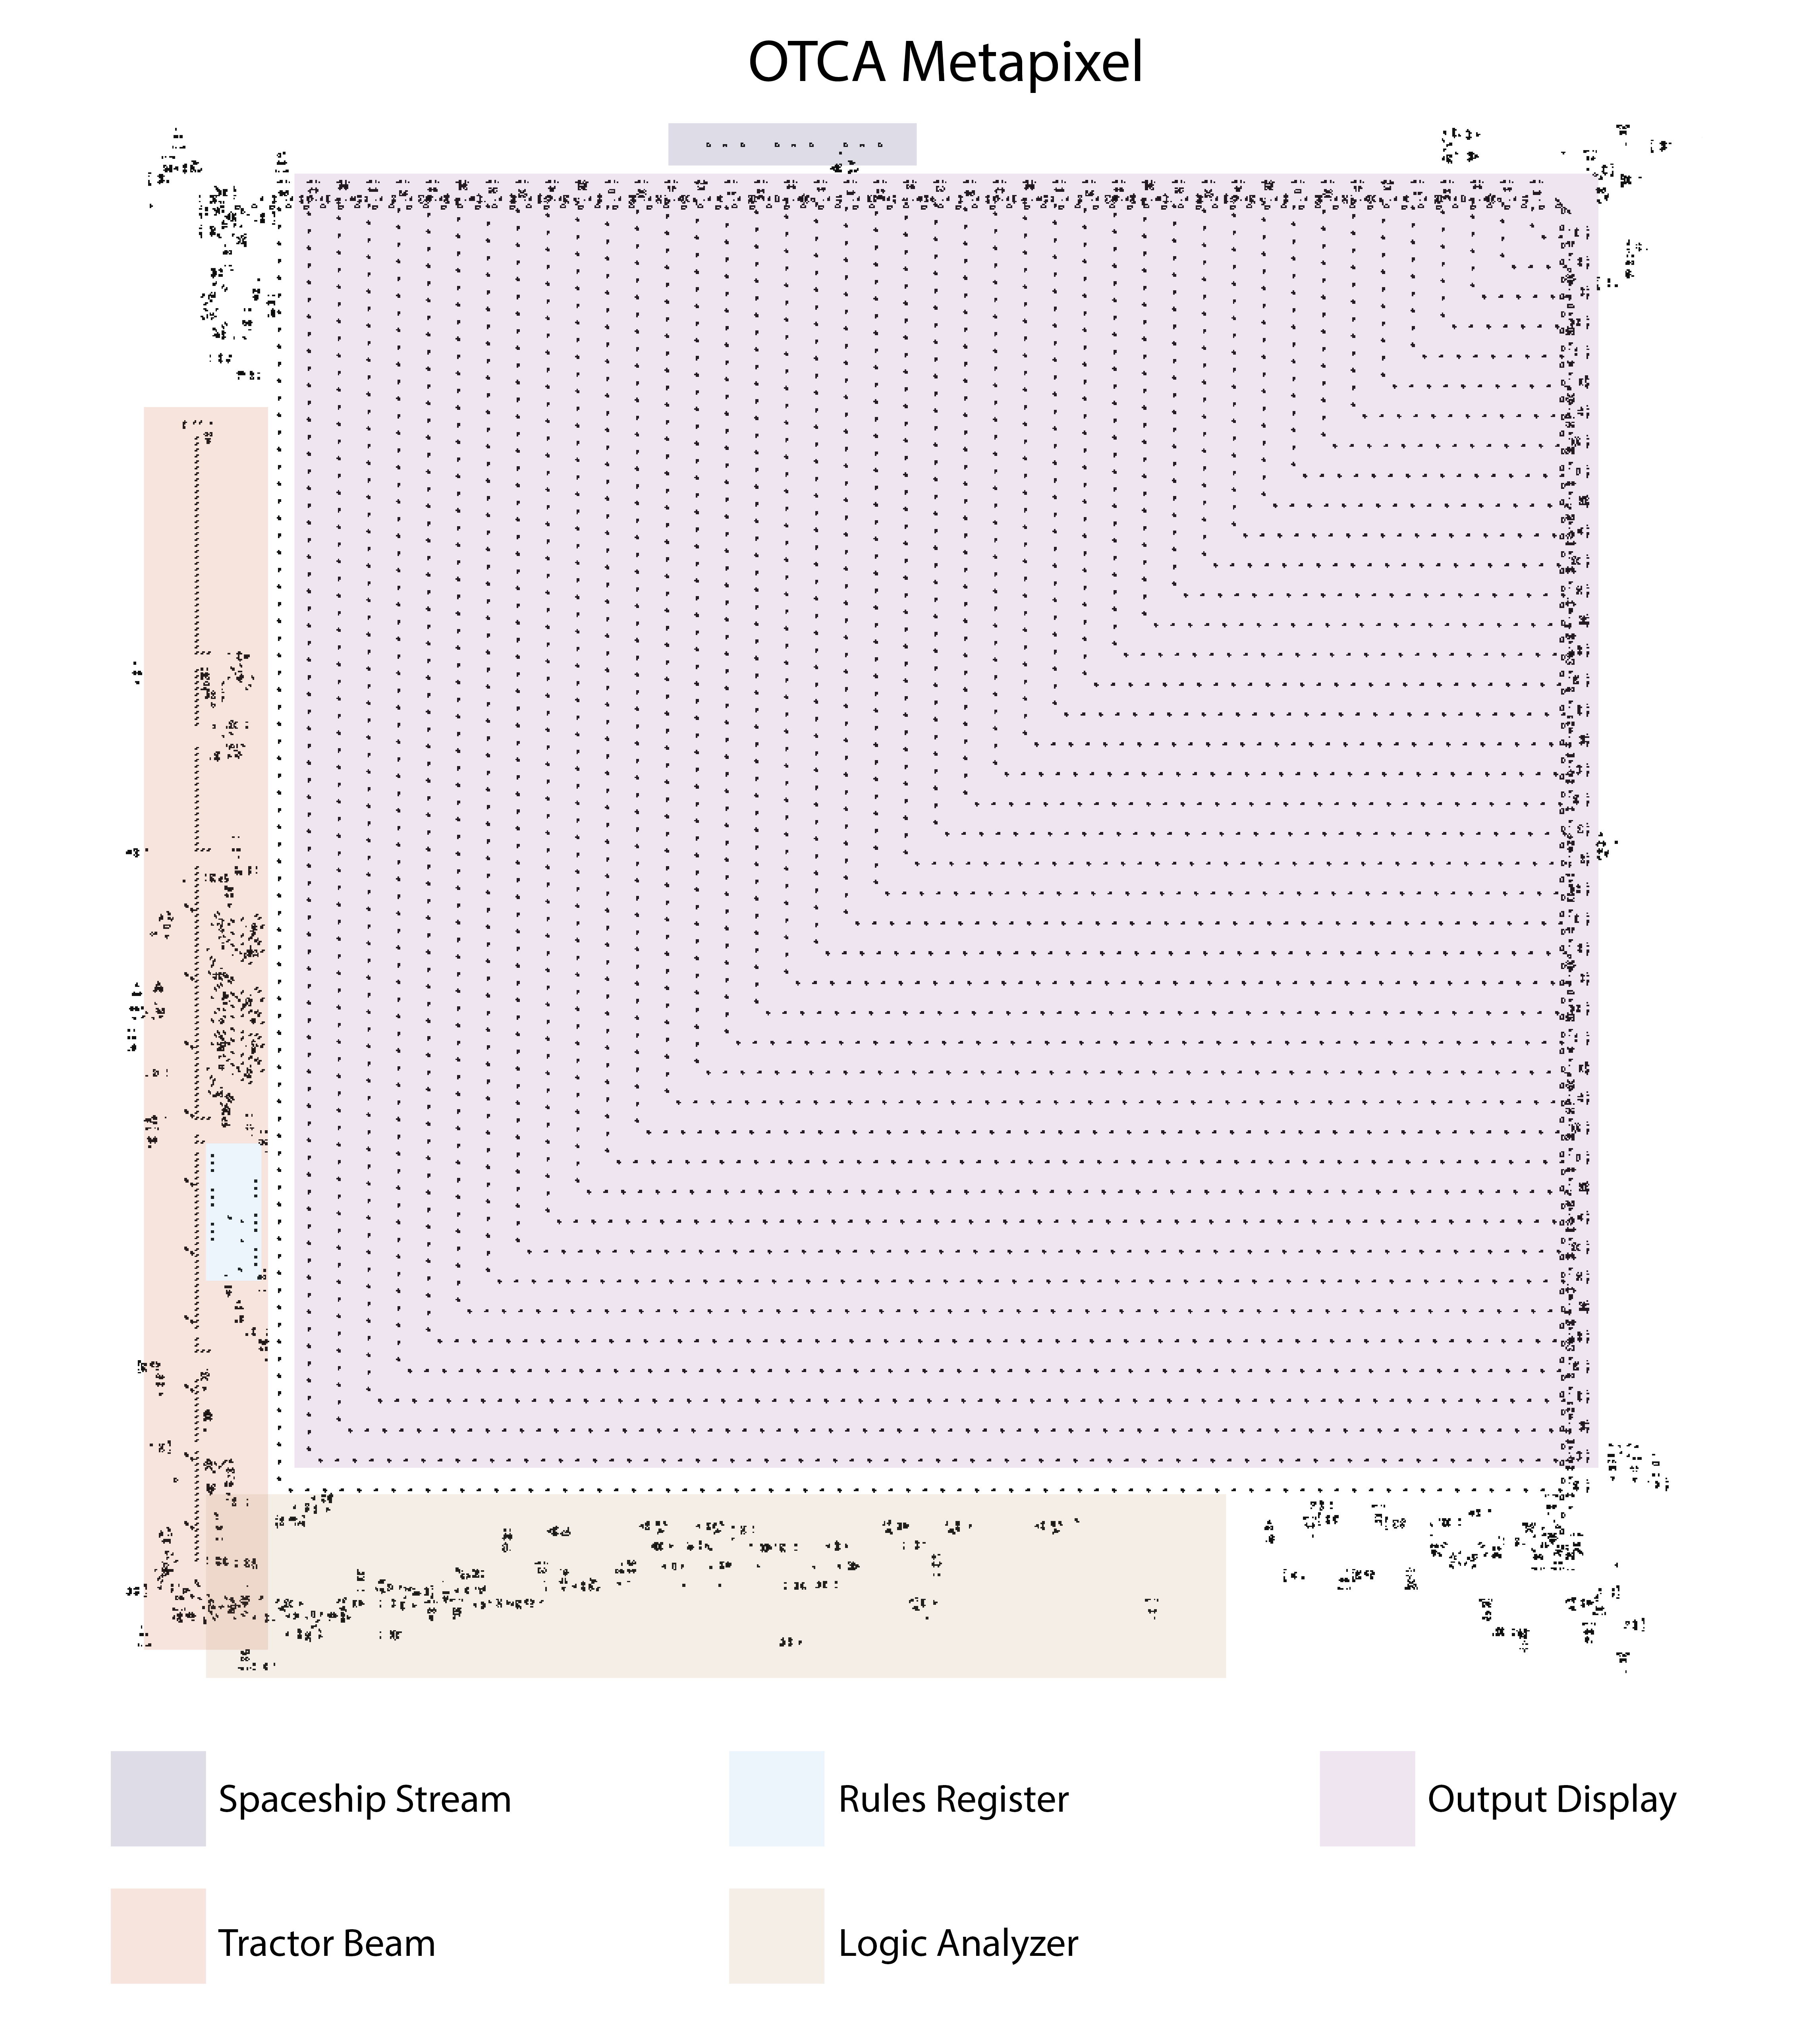
\includegraphics[width=\textwidth]{OTCADiagram.png}
  \caption{Complex-level diagram of OTCA Metapixel with the most important modules highlighted.}
  \label{fig:OTCADiagram}
\end{figure}



\section{Electronic Versus Mechanical Hierarchies}

scaling mismatch between the functional density of electronic and mechanical systems, offset in hierarchical setup.

\section{Hierarchy in Simulation}

increasing simulation abstraction as hierarchical level increases\\

In the next chapters, I'll describe the methods used to simulate assemblies of elements and functions, and describe how abstractions of the element-level simulation are adapted to the function-level.



}

%%% This is an example first chapter.  You should put chapter/appendix that you
%% write into a separate file, and add a line \include{yourfilename} to
%% main.tex, where `yourfilename.tex' is the name of the chapter/appendix file.
%% You can process specific files by typing their names in at the 
%% \files=
%% prompt when you run the file main.tex through LaTeX.

\singlespacing{

\chapter{Simulation of Parts}


}

%%% This is an example first chapter.  You should put chapter/appendix that you
%% write into a separate file, and add a line \include{yourfilename} to
%% main.tex, where `yourfilename.tex' is the name of the chapter/appendix file.
%% You can process specific files by typing their names in at the 
%% \files=
%% prompt when you run the file main.tex through LaTeX.

\singlespacing{

\chapter{Simulation}\label{chap:functionSim}

Simulation of function-level parts is carried out through a mass/spring/damper model.  In this model, neighboring face-connected cells apply forces and torques on one another through local interactions.  Translational and rotational positions and velocities are calculated from these forces using discrete-time integration techniques.  Internal degrees of freedom of \textit{functions} are parameterized by 15 stiffness and damping coefficients, $k$ and $d$.  Actuation is achieved by modulating the nominal distance of adjacent cells along a particular degree of freedom.  %In a sense, this type of simulation could be thought of as a dynamic constraint-solving system between solid elements with various degrees of freedom.

\section{Existing Models of Solids}

Mass/spring/damper
FEA

%Unlike traditional mass/spring/damper models of solids from computer graphics literature (cite stuff here), the model developed in this thesis draws on an abstraction of the functionality embedded in the different "function types".

\begin{figure}
  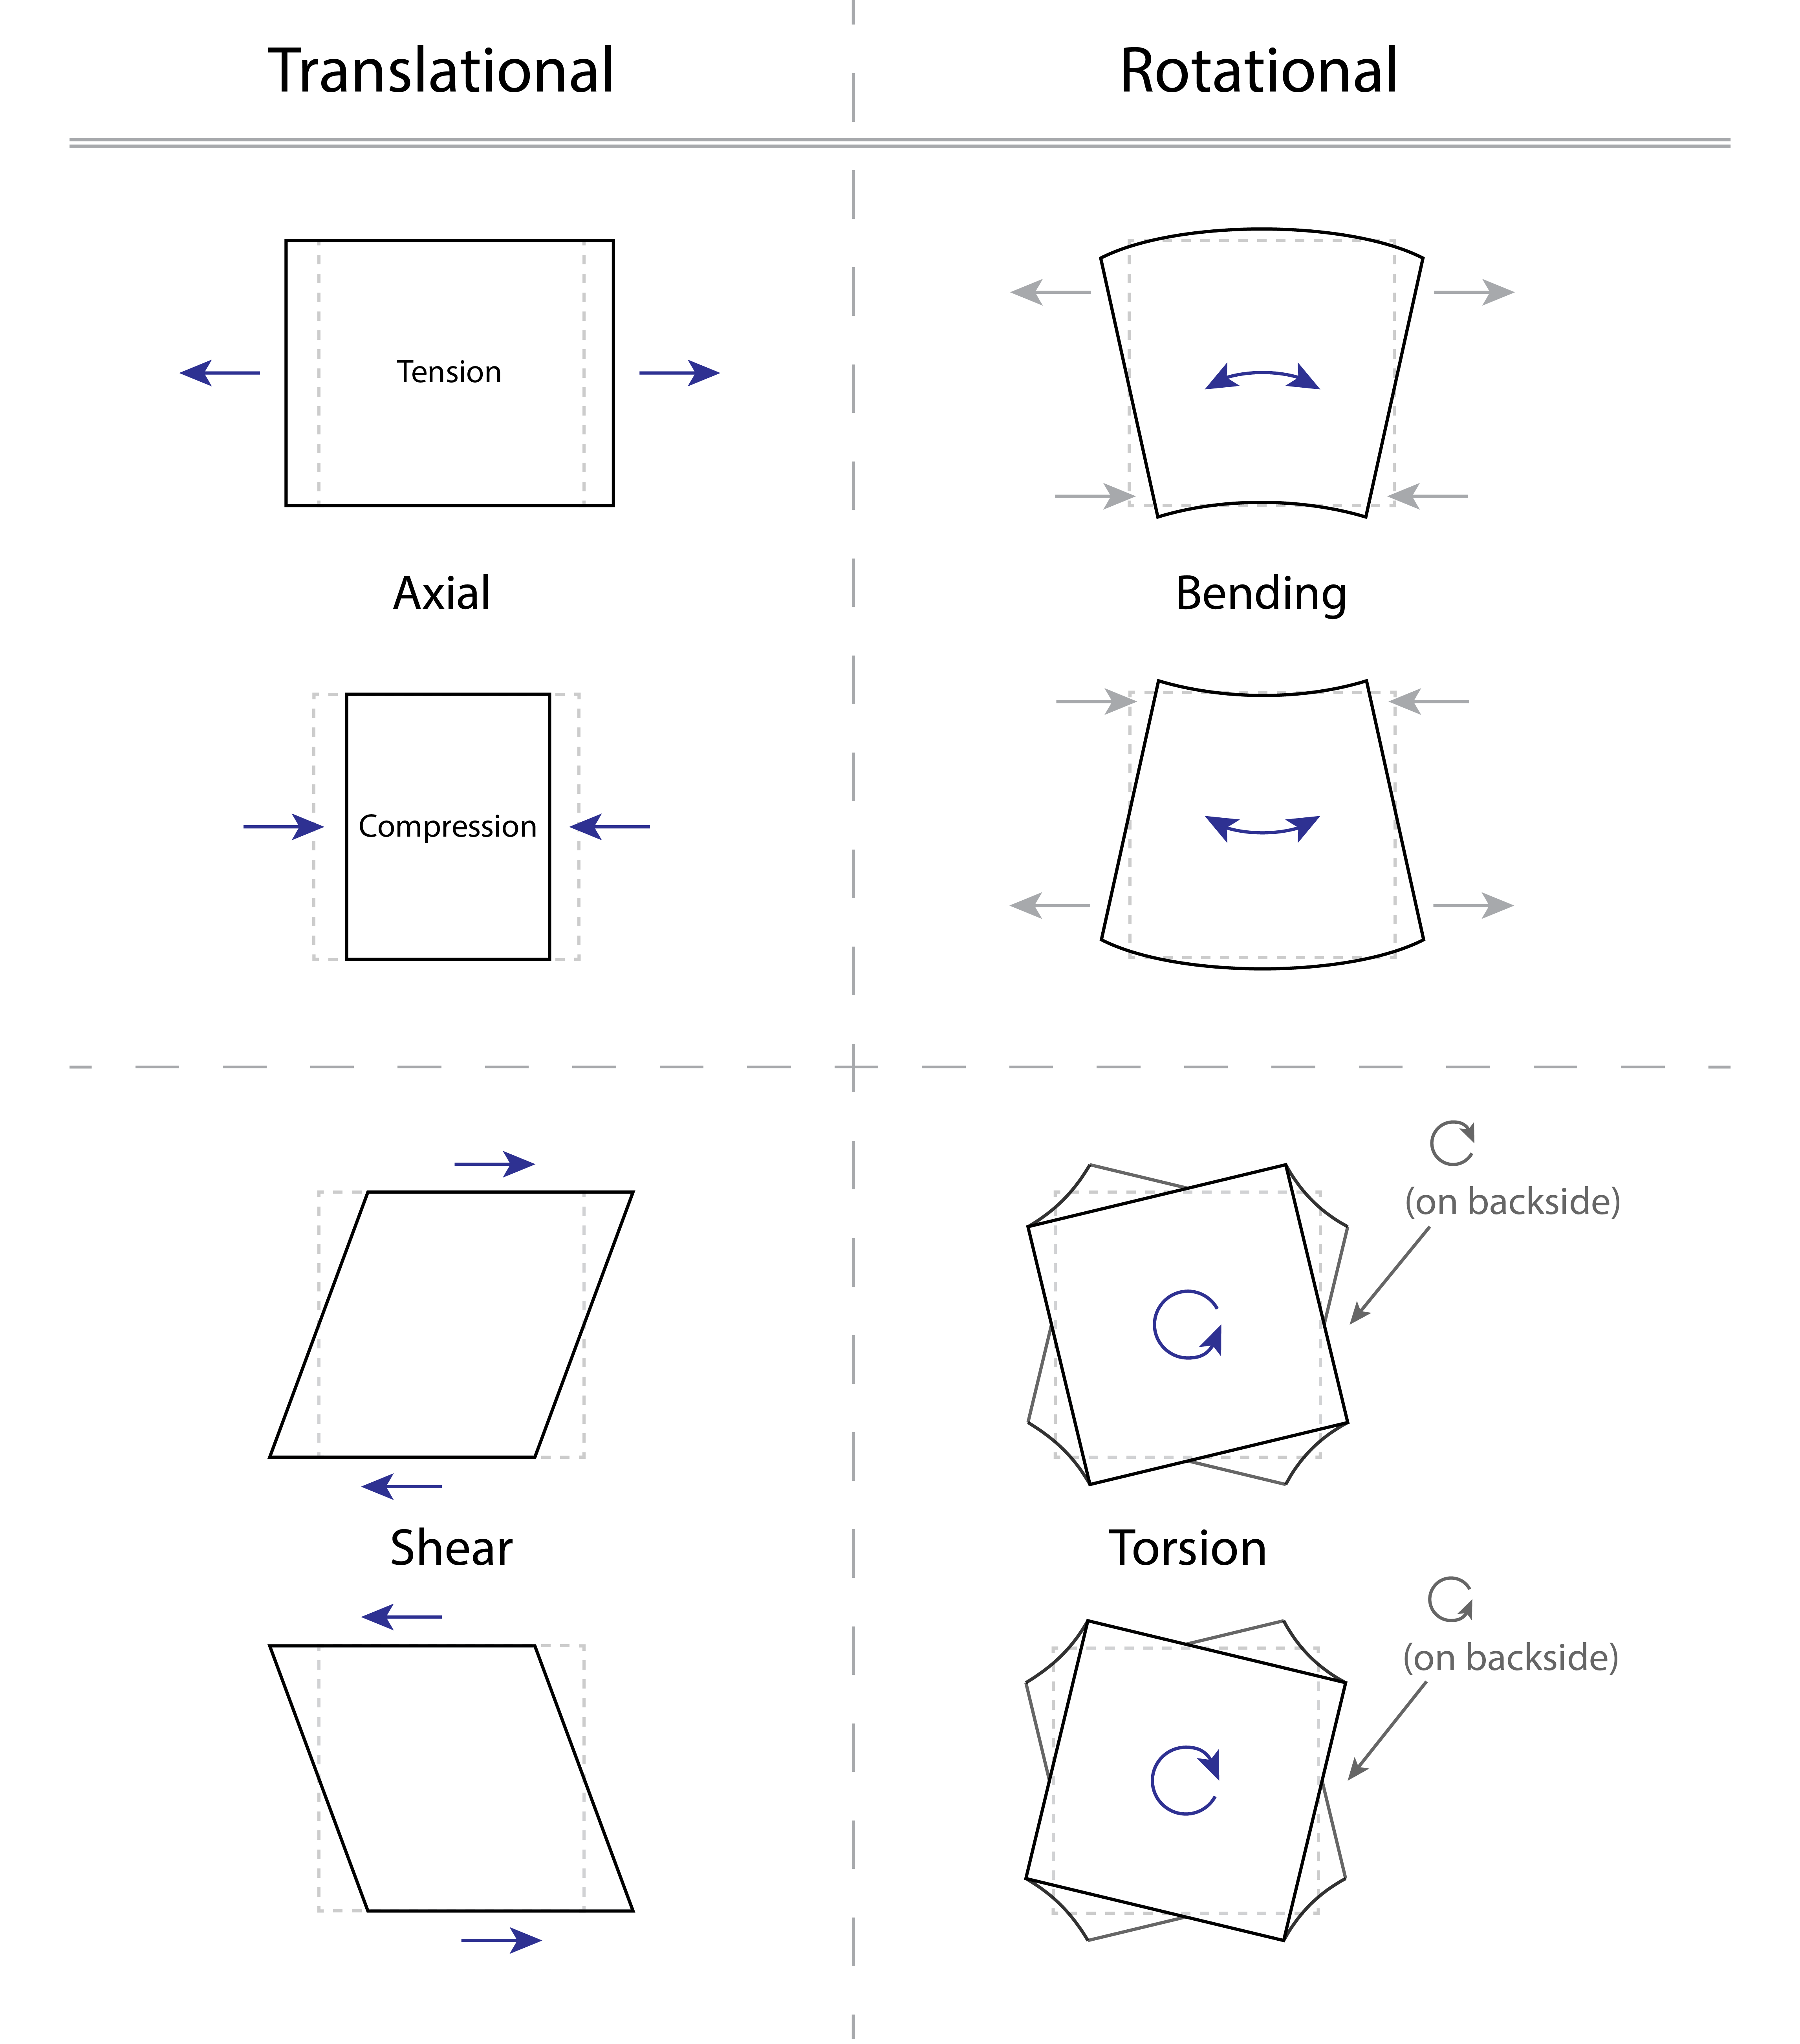
\includegraphics[width=\linewidth]{SolidMechanicsDOF.png}
  \caption{Deformations of a solid element under four types of applied forces.  In modeling assemblies of \textit{functions}, these characteristic deformations are referred to as "internal degrees of freedom".  Within an assembly of cells, longitudinal (compression and tension) and shear forces cause translational displacement and bending and torsional forces cause rotational displacement.}
  \label{fig:SolidMechanicsDOF}
\end{figure}

In solid mechanics, we can consider the global deformations of a solid as the summation of deformations of many smaller, discrete volumes, or \textit{finite elements}.  Forces acting on these finite elements fall into four categories: longitudinal (tension and compression), bending, shear, and torsion.  Each type of applied force causes a characteristic deformation of the finite element, illustrated in Figure \ref{fig:SolidMechanicsDOF}.  Applying multiple types of forces on a finite element will cause it to exhibit a combination of deformations.\\

In this model, simulation of an assembly happens at the granularity of identically-sized \textit{function}-level parts, which we'll call "cells".  When describing mechanical behavior of a particular cell type, we refer to its deformations as "internal degrees of freedom" (DOF).  For example, a 1-DOF bending cell will have large deformations in bending along one axis, but relatively small deformations in response to other types of applied forces.\\

\section{Function Types}

Cells at the function-level are defined not only by their mechanical properties, but also by their ability to transmit electronic signals from one face to another, and their active properties in response to a signal. The combinatorial space of mechanical, electronic, and actuated cell types is described in Figure \ref{fig:CombinatoricsOfFunctions}.  Section \ref{sec:electronicSim} describes the process of electronic simulation in more detail, the remainder of this chapter will focus on the passive and active mechanical simulation of function-level cells.
\\

\begin{figure}
  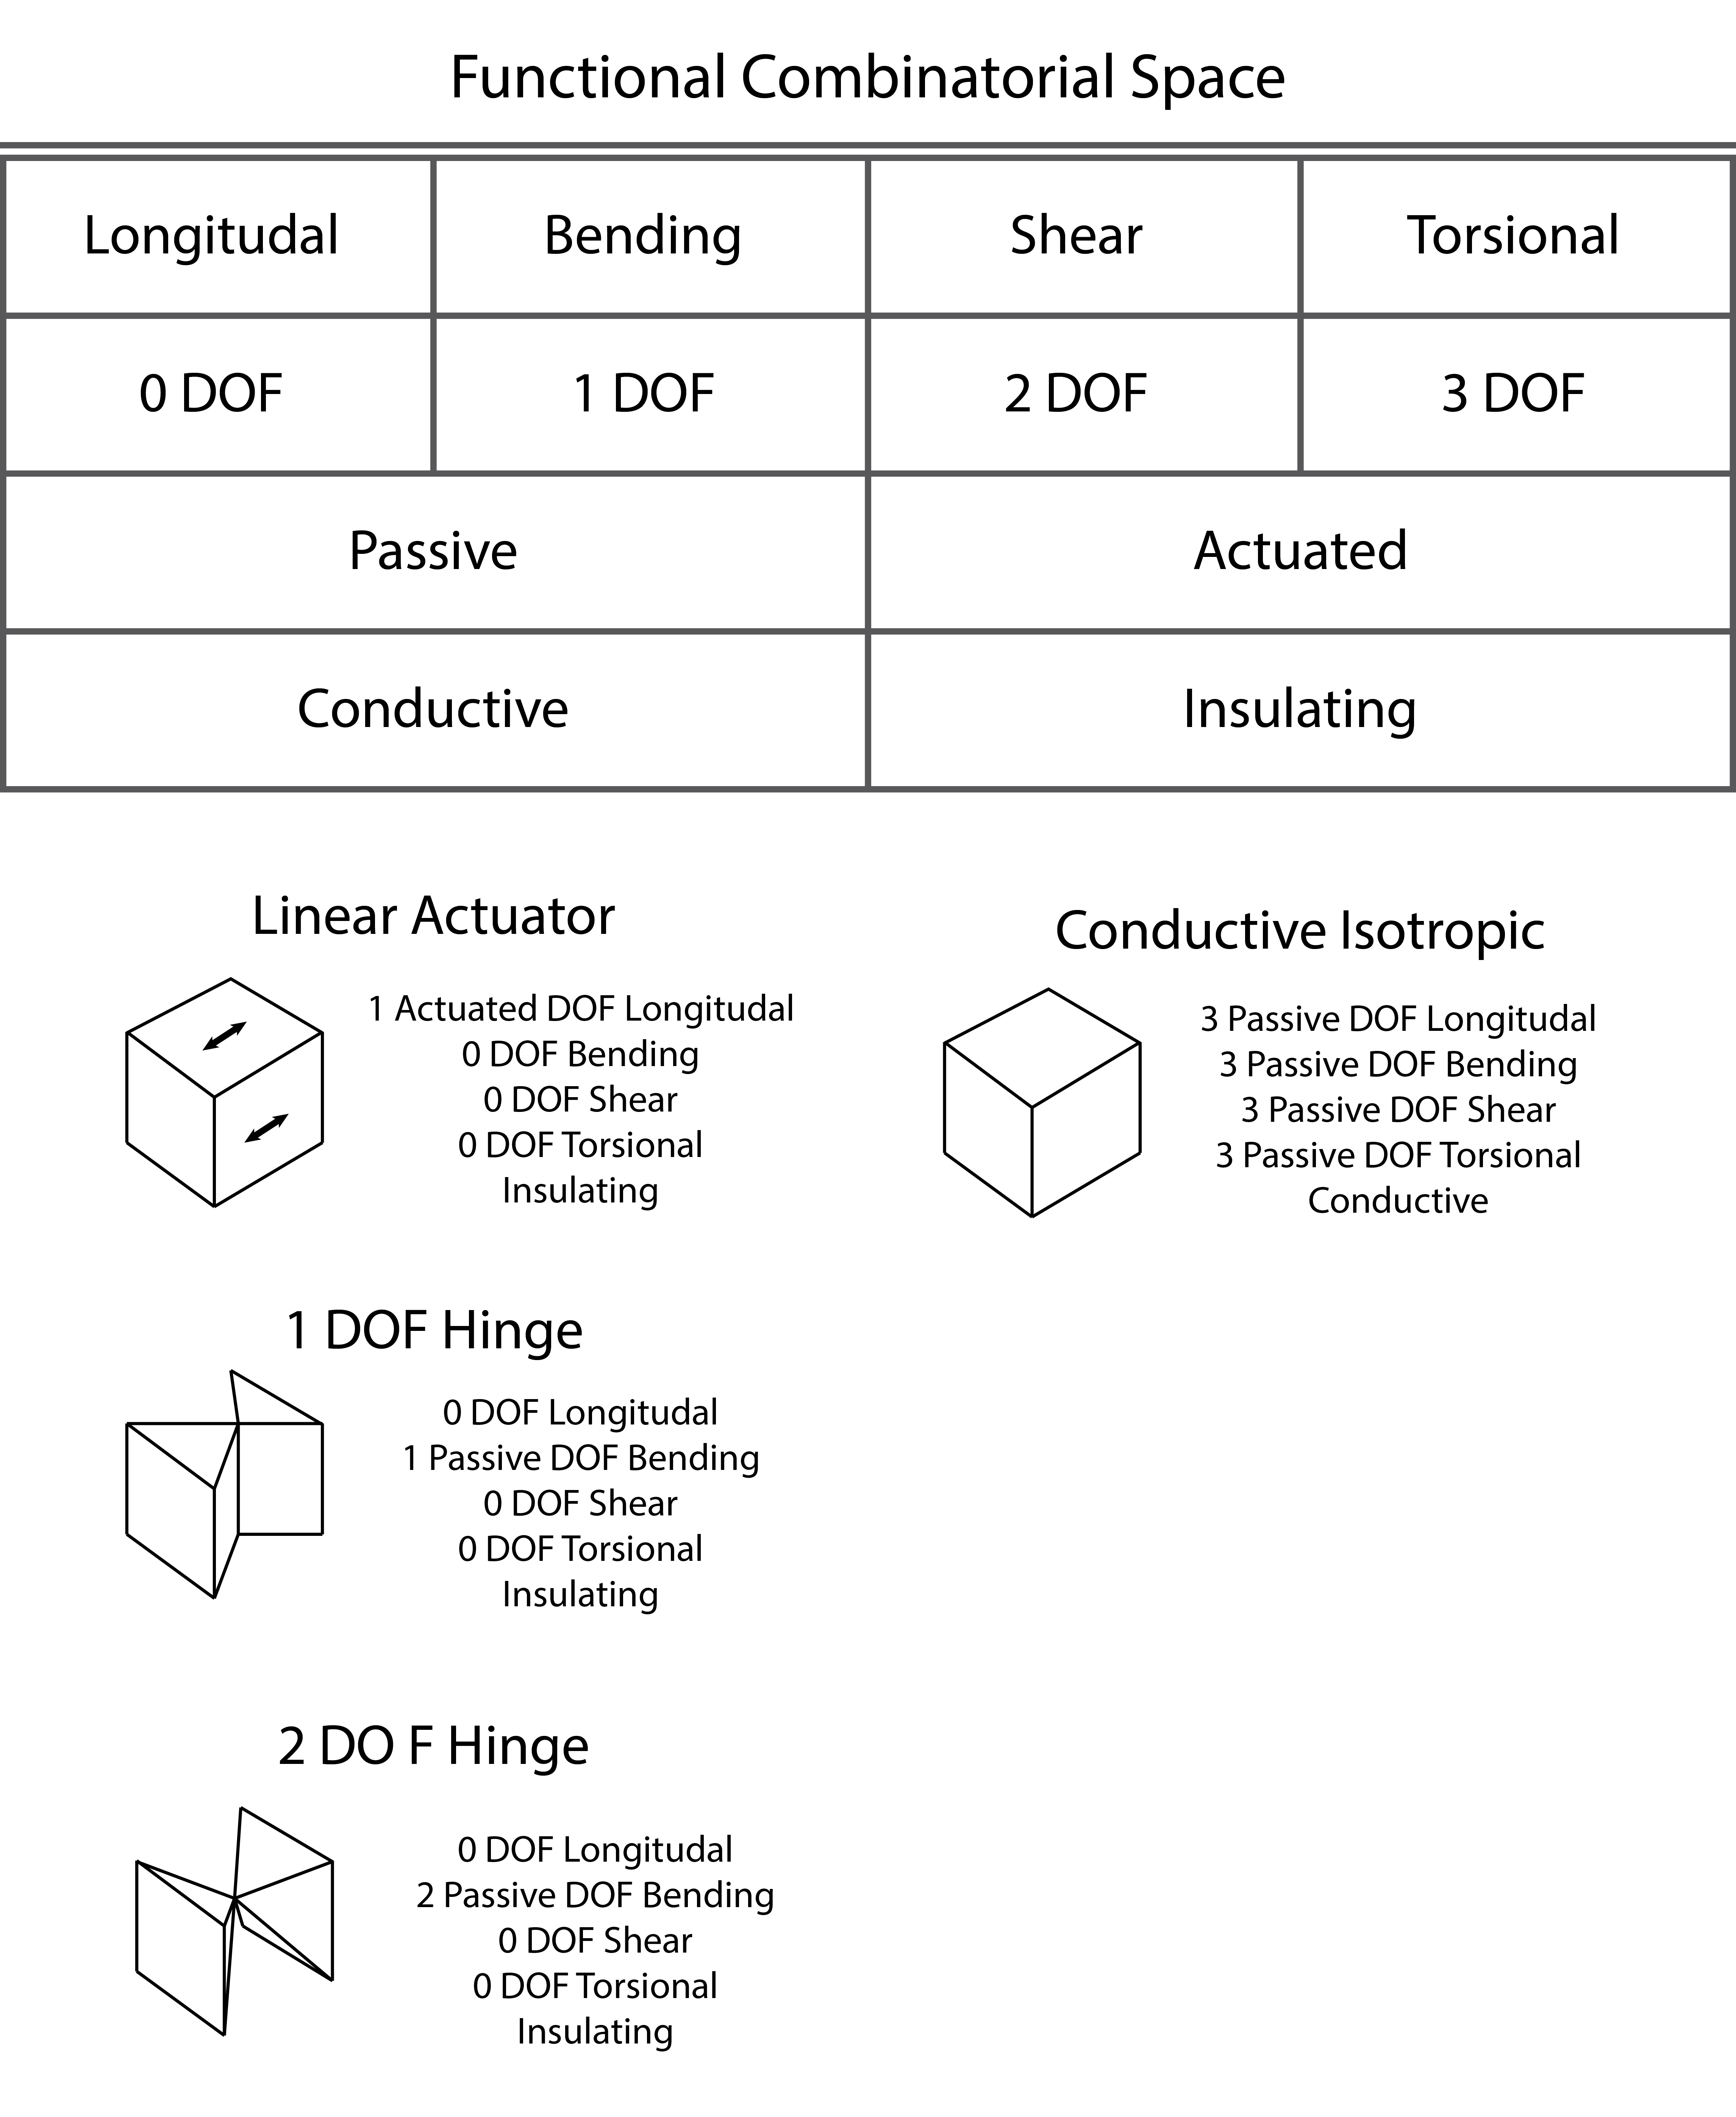
\includegraphics[width=\linewidth]{CombinatoricsOfFunctions.png}
  \caption{Combinatorial space of \textit{function} types with six examples explicitly described in terms of their electronic and mechanical properties.  Note - any individual degree of freedom within a cell falls on the spectrum described in Figure \ref{fig:BendingStiffnessContinuoum}.  A cell is described at a high level as having a particular degree of freedom if its corresponding stiffness in that dimension is sufficiently flexible to allow for significant deformation uder applled load.  There are no infinitely stiff or fully unconstrained degrees of freedom in this system.}
  \label{fig:CombinatoricsOfFunctions}
\end{figure}

\section{Geometric Stiffness}

The geometric stiffness of a structure relates the bulk properties of a material to its 3d geometry.  For example, an I-beam has a higher geometric bending stiffness than an equal length rectangular bar made from the same amount of the same material.  Unless otherwise noted, "stiffness" in this analysis refers to geometric stiffness.\\

Stiffness and damping are used to characterize the response of cell's internal degrees of freedom to applied external forces.  In three dimensions, each cell's passive mechanical properties are parameterized by 15 stiffness and damping constants:

\[ k  \left\{ \begin{array}{ccc}
k_{longitudinal_x}\\
k_{longitudinal_y}\\
k_{longitudinal_z}\\
\\
k_{shear_{xy}}\\
k_{shear_{xz}}\\
k_{shear_{yx}}\\
k_{shear_{yz}}\\
k_{shear_{zx}}\\
k_{shear_{zy}}\\
\\
k_{bending_x}\\
k_{bending_y}\\
k_{bending_z}\\
\\
k_{torsional_x}\\
k_{torsional_y}\\
k_{torsional_z}
 \end{array} \right\} 
 \qquad\qquad
 d  \left\{ \begin{array}{ccc}
d_{longitudal_x}\\
d_{longitudal_y}\\
d_{longitudal_z}\\
\\
d_{shear_{xy}}\\
d_{shear_{xz}}\\
d_{shear_{yx}}\\
d_{shear_{yz}}\\
d_{shear_{zx}}\\
d_{shear_{zy}}\\
\\
d_{bending_x}\\
d_{bending_y}\\
d_{bending_z}\\
\\
d_{torsional_x}\\
d_{torsional_y}\\
d_{torsional_z}
 \end{array} \right\}  \]
\\

$k_{shear}$ and $d_{shear}$ are broken out into six parameters of the form $shear_{nm}$ because the shear response depends both on the direction of shear displacement between two cells ($m$) and on the axis along which the cells are connected ($n$).  The $shear_{nm}$ notion used above is described graphically in in Figure \ref{fig:ShearDOFs}.\\

\begin{figure}
  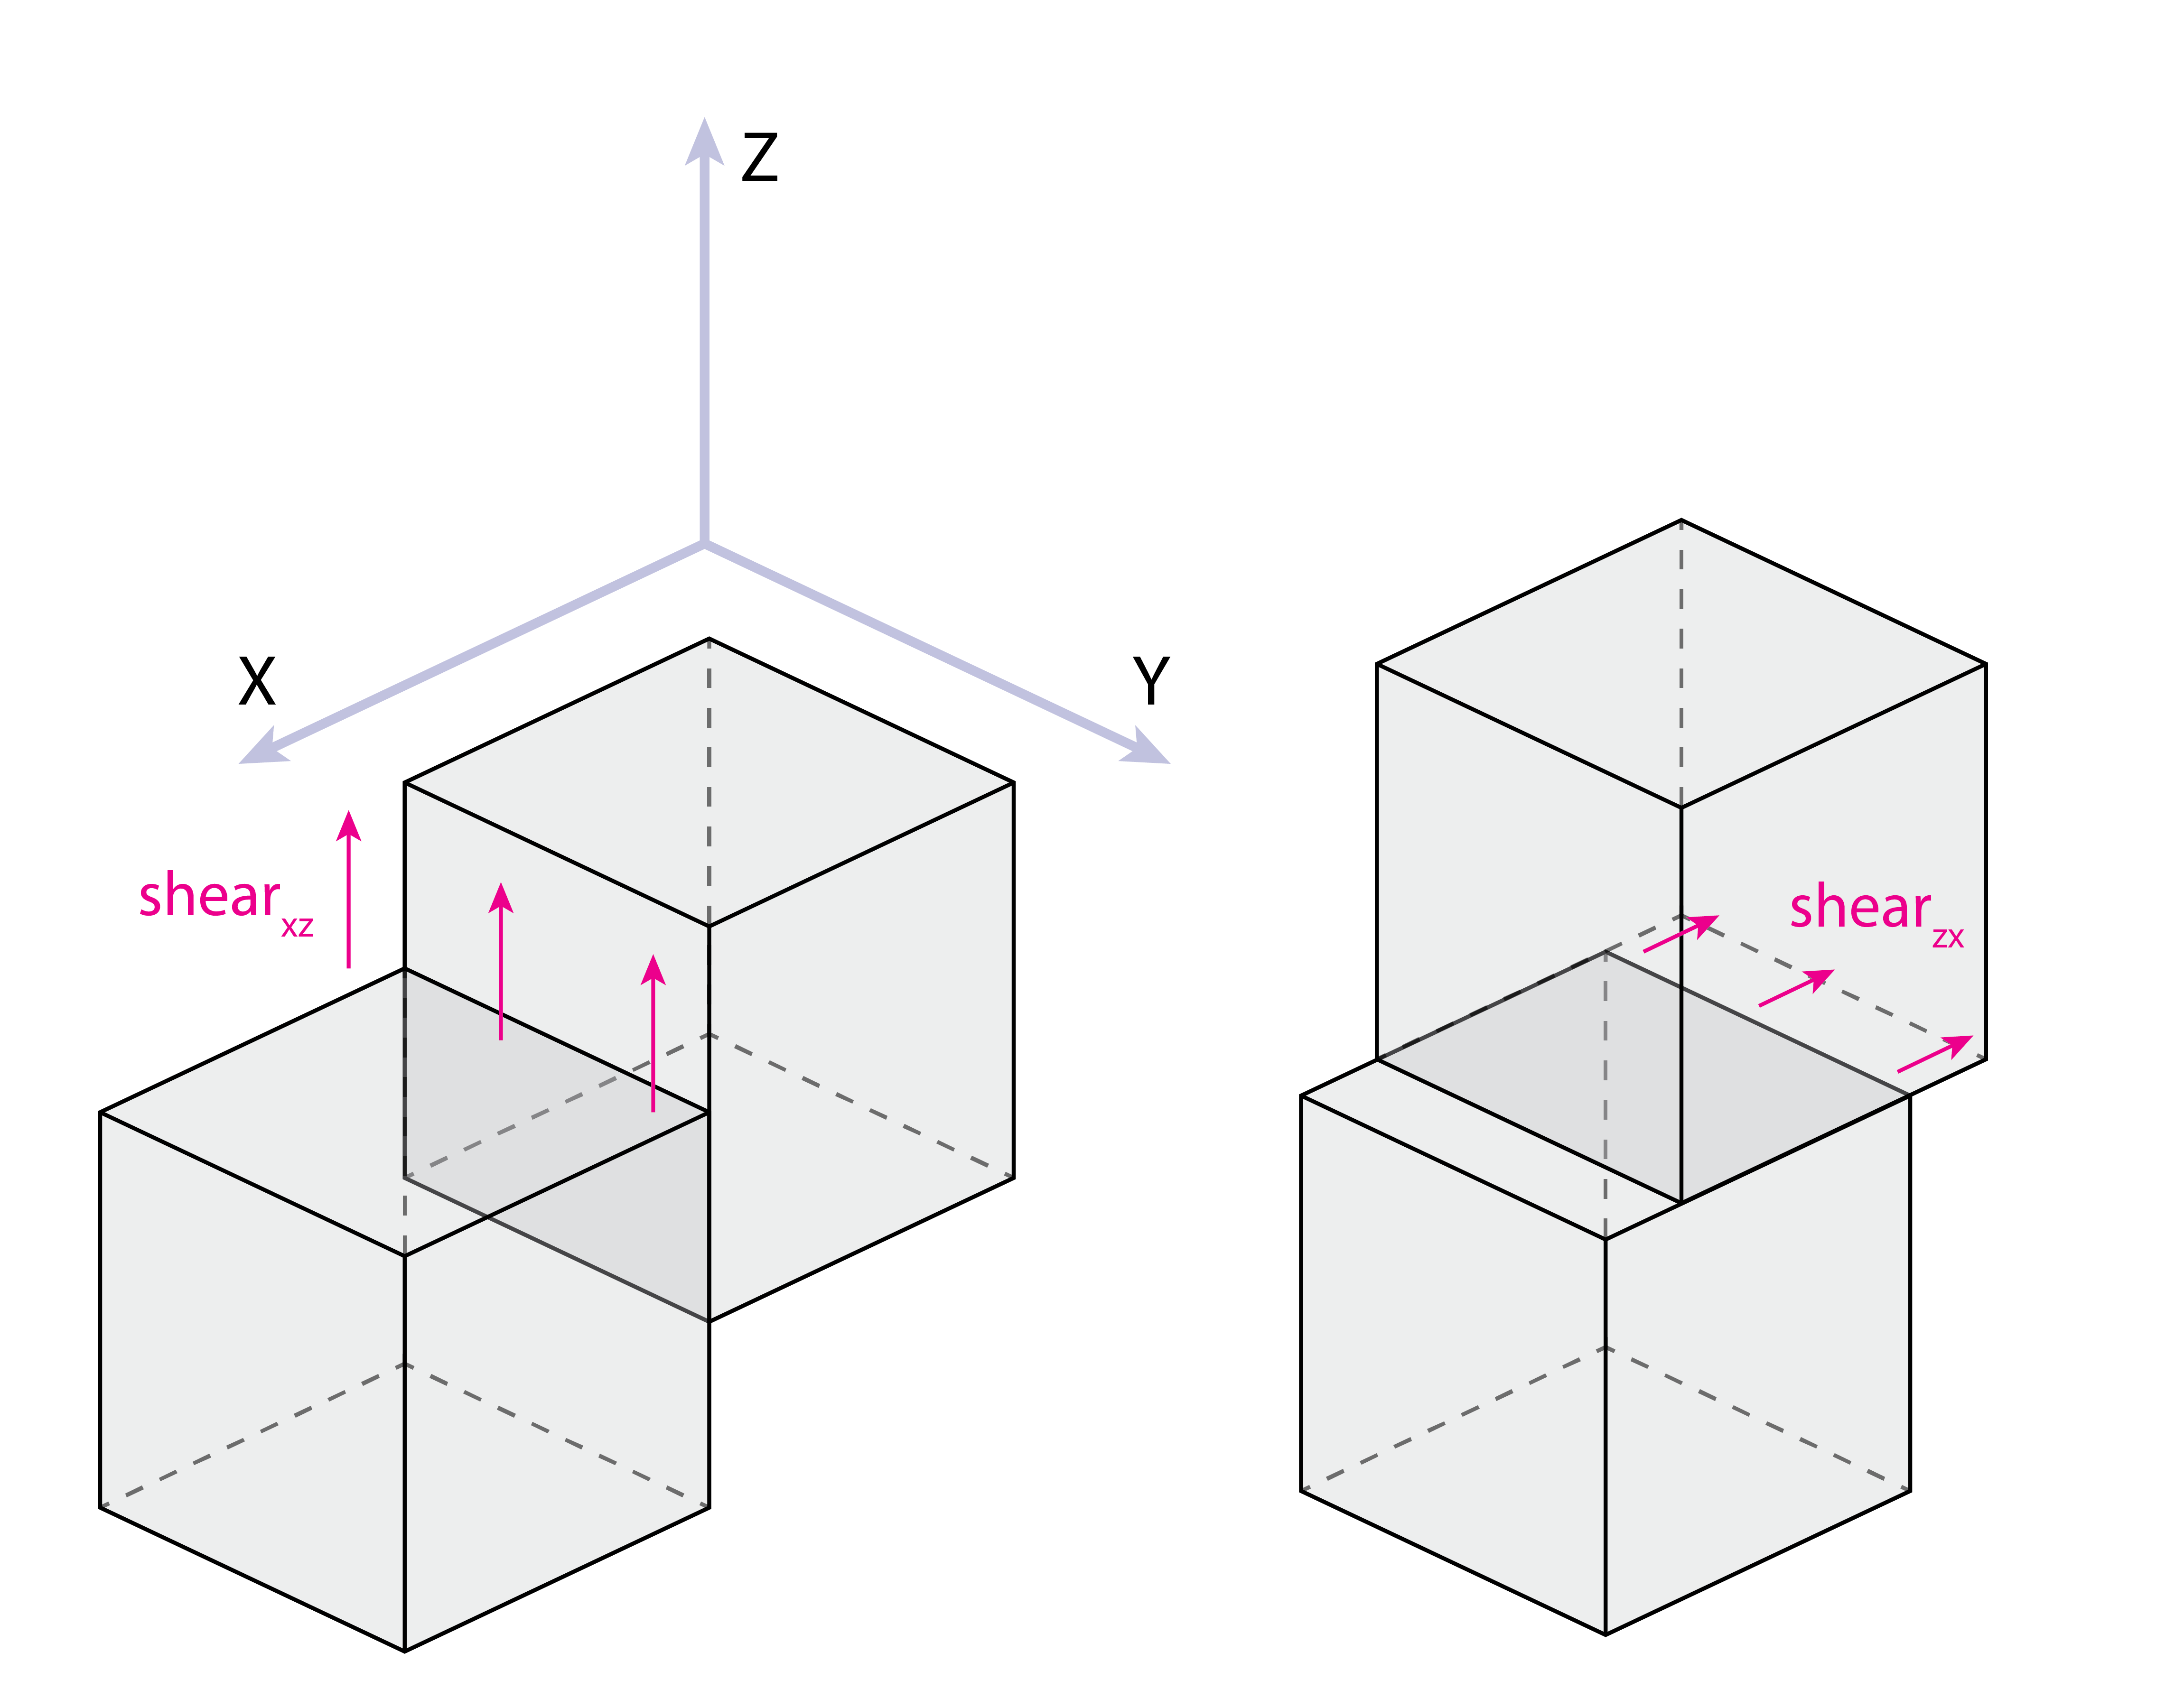
\includegraphics[width=\linewidth]{ShearDOFs.png}
  \caption{Illustration of shear subscript notation.  First subscript describes the direction of neighboring cell connection, second describes the direction of shear displacement.}
  \label{fig:ShearDOFs}
\end{figure}

The stiffness and damping constants of each cell type may be calculated from bulk properties of the constituent materials that make up the cell, or they may be measured empirically.  For example, an isotropic cell made from a bulk material with elastic modulus $E$ and shear modulus $G$ has stiffnesses defined by:

\[ k_{longitudinal} = \dfrac{aE}{l}\]
\[ k_{shear} = \dfrac{Ga}{l} ??\]
\[ k_{torsion} = \dfrac{GJ}{l}\]
\[ k_{bending} = \dfrac{aE}{l} ??\]
\\
where $a$ is the cross sectional area and $l$ is the length of the ce;;.\\

A linear scale showing the range of physically achievable 1-DOF bending cell types compared with the range of theoretically possible types is shown in Figure \ref{fig:BendingStiffnessContinuoum}.  Due to manufacturing and material constraints, we do not envision \textit{function}-level cells that occupy the region near zero bending stiffness (e.g. a frictionless pin joint) or infinite bending stiffness (zero compliance material).

\begin{figure}
  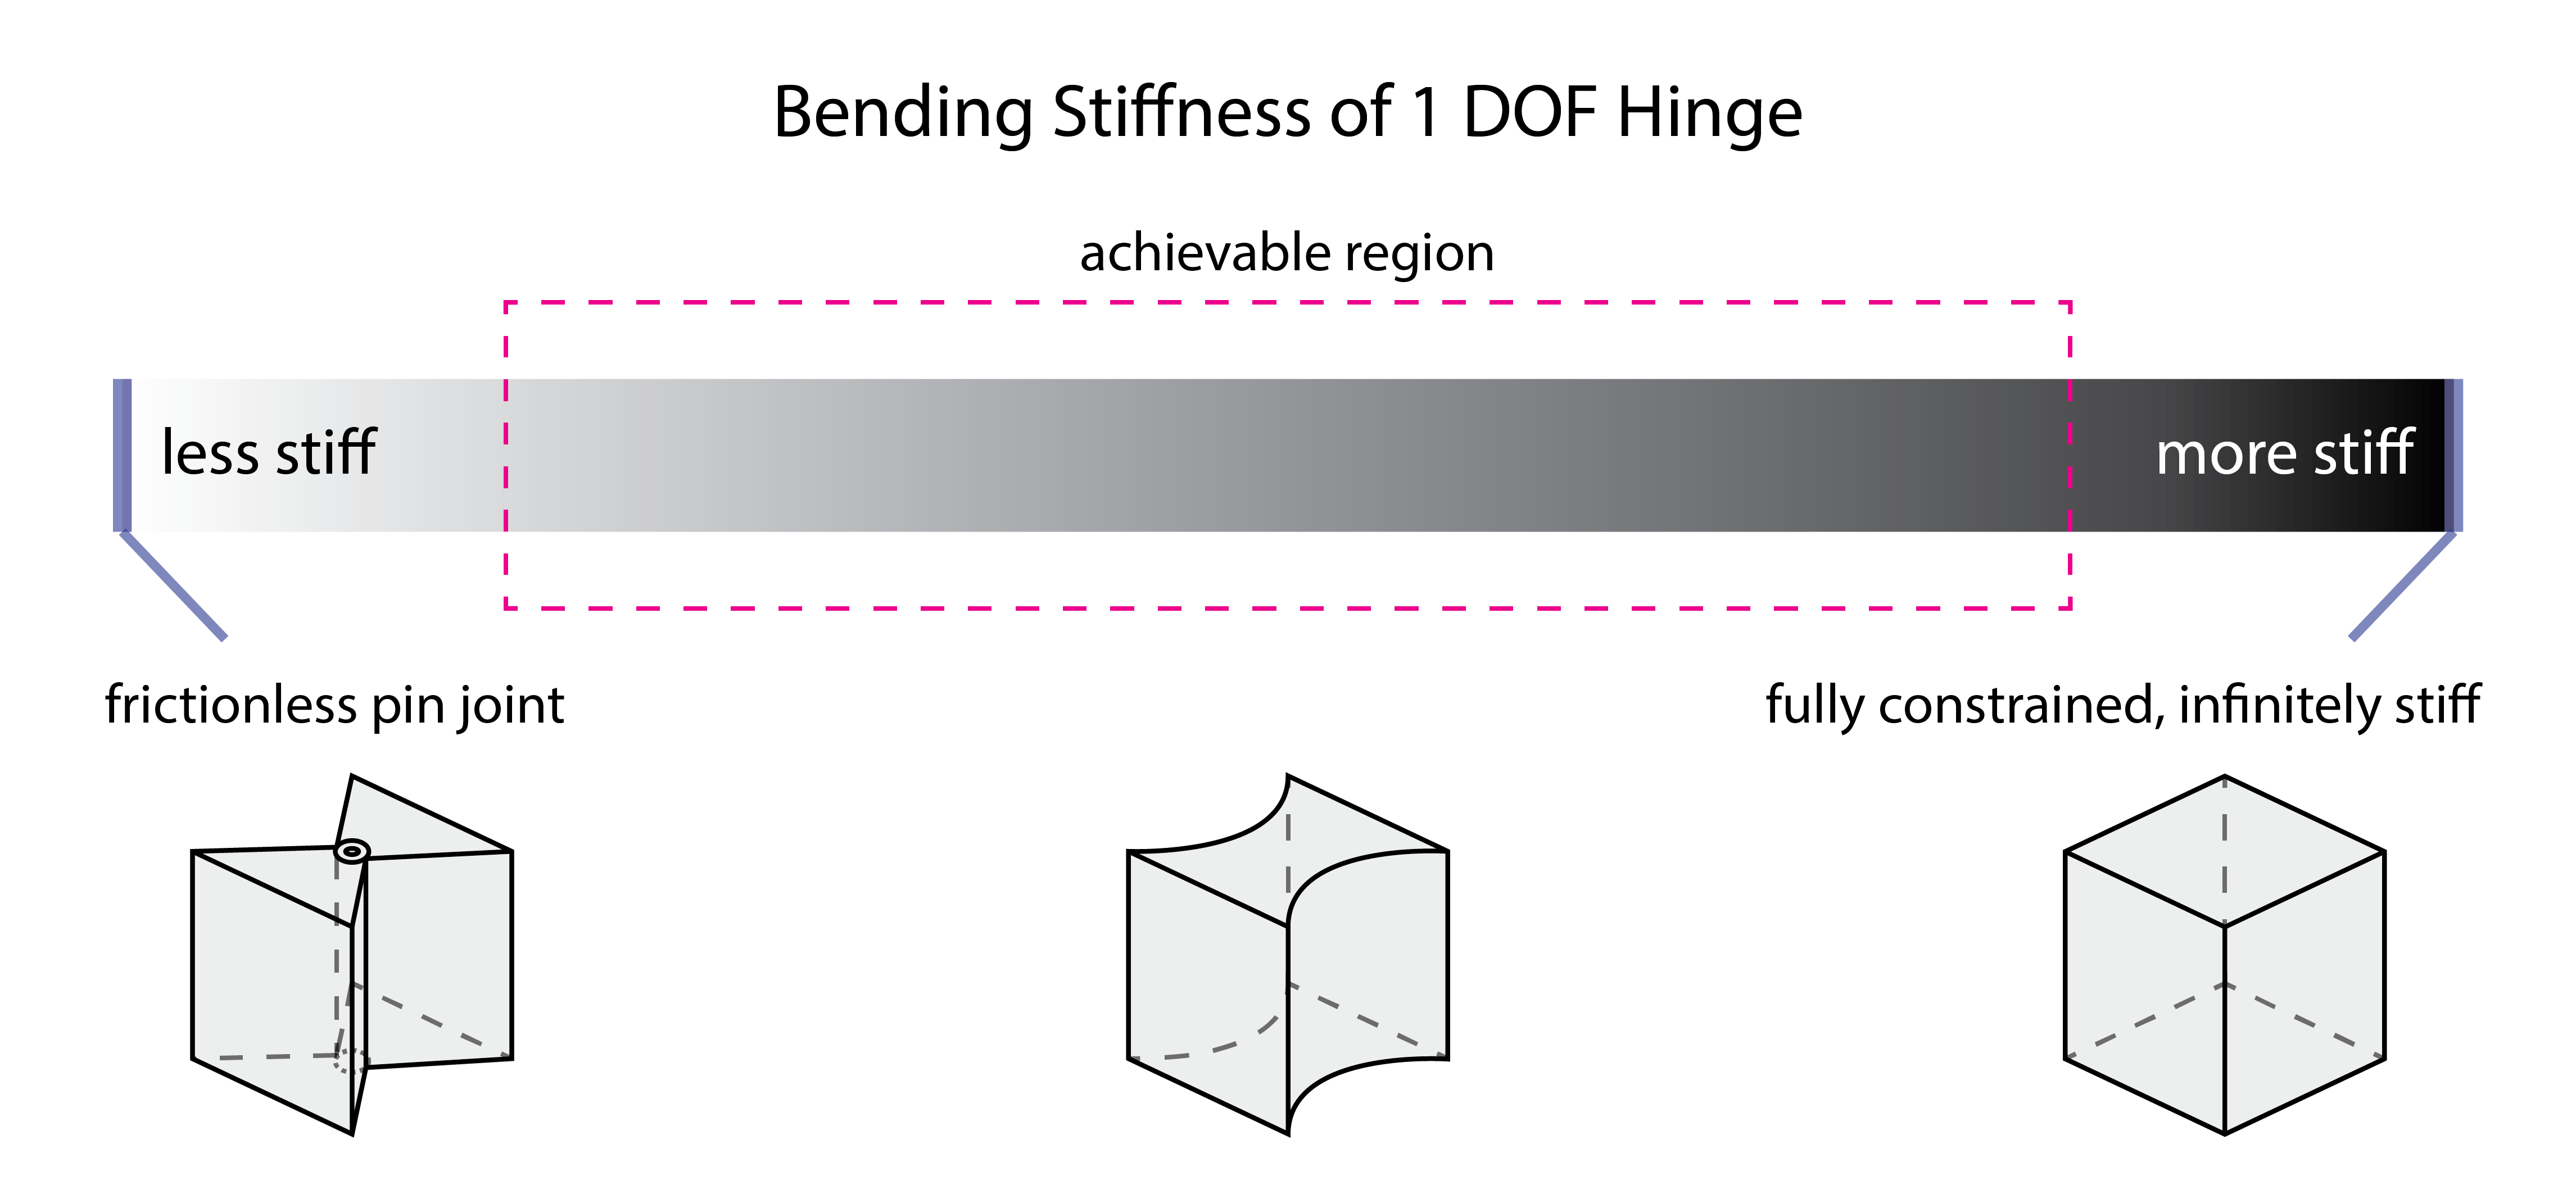
\includegraphics[width=\linewidth]{BendingStiffnessContinuoum.png}
  \caption{Continuum of bending stiffness in a 1 DOF hinge.}
  \label{fig:BendingStiffnessContinuoum}
\end{figure}


\section{Translational Forces}

In the simplest case without rotation, the force $f_{1 \rightarrow 2}$ applied to cell 2 by cell 1 is given by:

\begin{figure}
  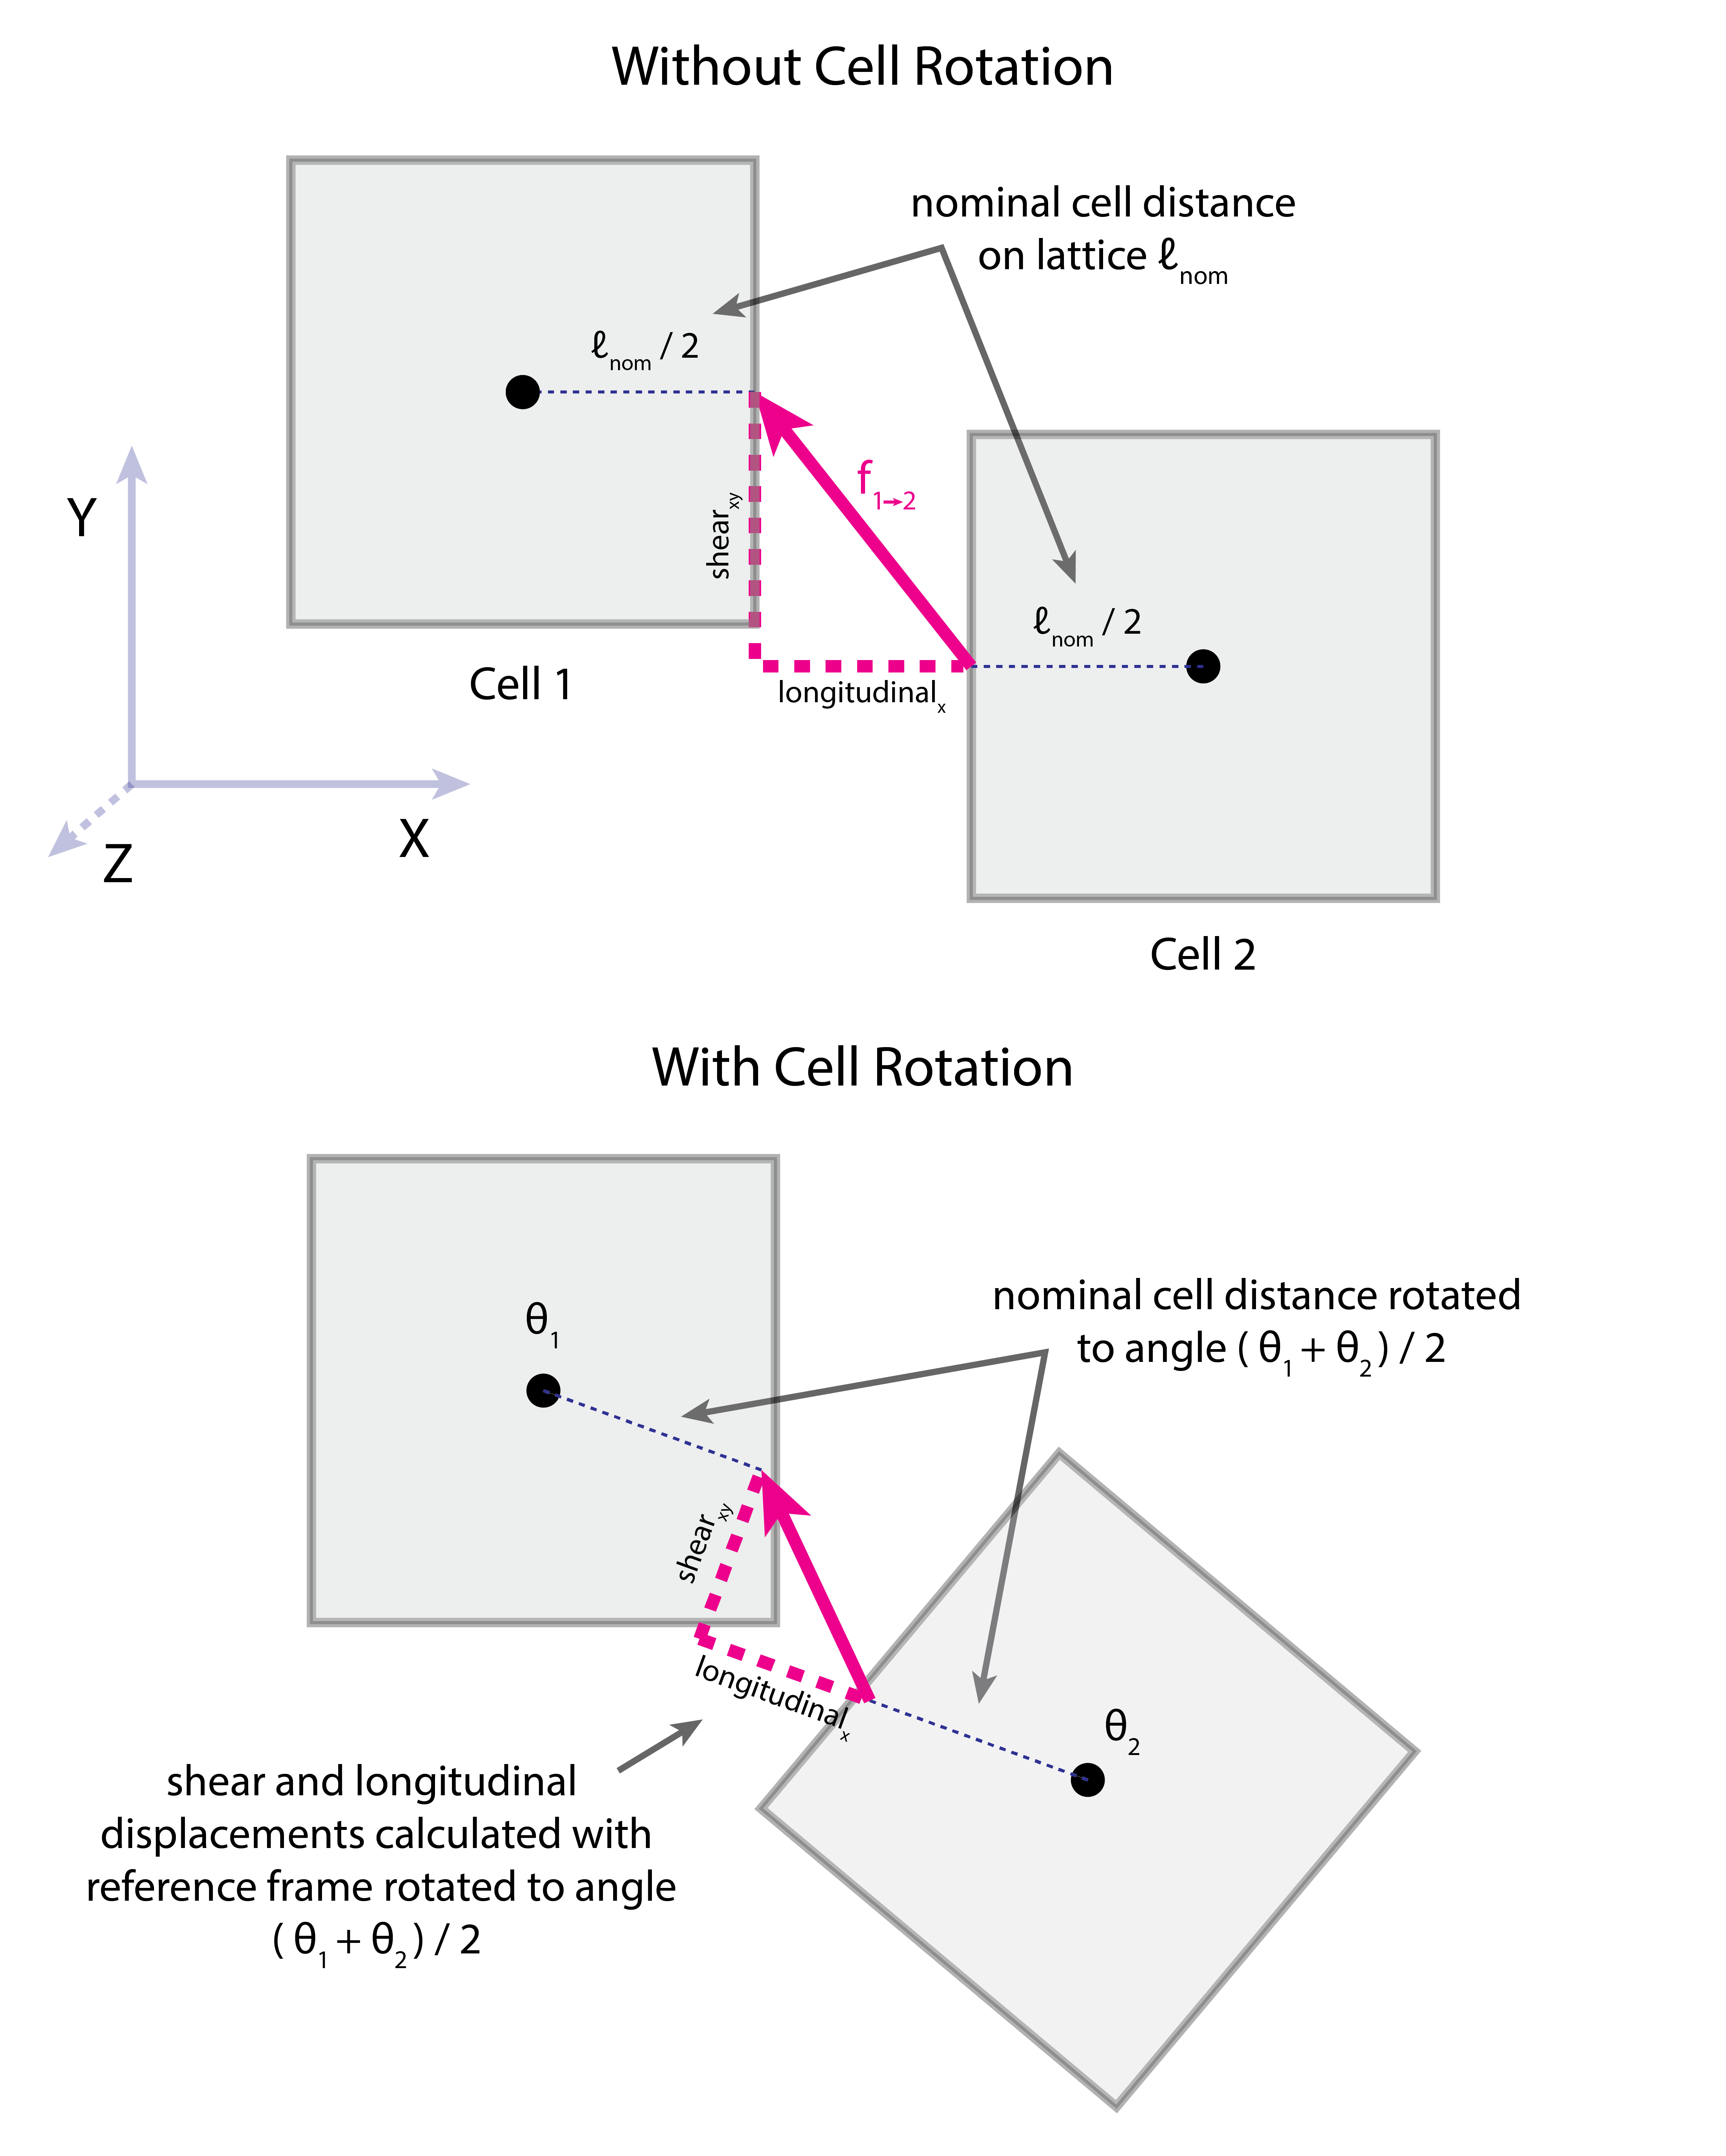
\includegraphics[width=\linewidth]{translationalSim.png}
  \caption{translationalSim.}
  \label{fig:translationalSim}
\end{figure}

\begin{equation} \label{eq:translationalForce}
\vec{f_{1\rightarrow2}} = \vec{k} \circ (\vec{p_2} - \vec{p_1}) + \vec{d} \circ (\vec{v_2} - \vec{v_1})
\end{equation}
where $\vec{p_1}$ and $\vec{p_2}$ are the displacements of cell 1 and cell 2 from their nominal position in the lattice, $\vec{v_1}$ and $\vec{v_2}$ are the cells' translational velocities, $\circ$ is multiplication of two vectors by element, and $\vec{k}$ and $\vec{d}$ are 3D vectors containing the appropriate stiffness and damping constants for the interaction between the cells.  For example, given the scenario illustrated in Figure \ref{fig:translationalSim}, where two cells are connected along the x axis, a longitudinal constant should be used for displacements along x and shear constants should be used for displacements along y and z:
\[ k =  \left[ \begin{array}{ccc}
k_{longitudinal_x}\\
k_{shear_{xy}}\\
k_{shear_{xz}}
 \end{array} \right]  
  \qquad\qquad
  d =  \left[ \begin{array}{ccc}
d_{longitudinal_x}\\
d_{shear_{xy}}\\
d_{shear_{xz}}
 \end{array} \right] \]\\
 
If we wish to consider the orientations of the cells, denoted by the unit quaternions $q1$ and $q2$, we will need to adjust equation \ref{eq:translationalForce}. \\
  
  We can rotate a vector $v$ in 3-space by a quaternion $q$ in 4-space:
    \[ v_{rotated} = q*v*q^* \]
  
  by treating $v$ as a 4-space vector [x, y, z, w] with w=0, with $*$ denoting the Hamilton product:
  \[ a*b =  \left[ \begin{array}{ccc}
a_wb_x + a_xb_w + a_yb_z - a_zb_y\\
a_wb_y - a_xb_z + a_yb_w + a_zb_x\\
a_wb_z + a_xb_y - a_yb_x + a_zb_w\\
a_wb_w - a_xb_x - a_yb_y - a_zb_z
 \end{array} \right] \] 
 
   and $q^*$ denoting the conjugate of $q$:
    \[ q^{*} =  \left[ \begin{array}{ccc}
-q_x\\
-q_y\\
-q_z\\
q_w
 \end{array} \right] \] 
 
By performing a spherical linear interpolation (slerp) halfway between $q1$ and $q2$, we can calculate the average orientation of the two cells as a unit quaternion:
  \[ q_{avg} = slerp(q_{1}, q_{2}; 0.5) \]
  
Using $q_{avg}$, we can rotate the stiffness and damping vectors from Equation \ref{eq:translationalForce} into this average reference frame, and substitute the rotated vectors back into equation \ref{eq:translationalForce}:

 \[ \vec{k_{rot}} = (q_{avg}*\vec{k}*q_{avg}^*)\]
  \[ \vec{d_{rot}} = (q_{avg}*\vec{d}*q_{avg}^*)\]
  \begin{equation} \label{eq:translationalForceRotStep}
 \vec{f_{1\rightarrow2}} = \vec{k_{rot}} \circ (\vec{p_2} - \vec{p_1}) + \vec{d_{rot}} \circ (\vec{v_2} - \vec{v_1})
 \end{equation}
 
Finally, we need to make an adjustment to the nominal differential position between the cells, indicated in Figure \ref{fig:translationalSim}.  The form above assumes the nominal distance between the centers of the cells is the unrotated distance between them in their initial lattice configuration, $\vec{l_{nom}}$.  Rotating $\vec{l_{nom}}$ into the average rotational reference frame of the two cells gives
 \[\vec{l_{rot}} = q_{avg}*\vec{l_{nom}}*q_{avg}^*\]
 
introducing this to Equation \ref{eq:translationalForceRotStep} gives the final form:
 \begin{equation} \label{eq:translationalForceRot}
  \vec{f_{1\rightarrow2}} = \vec{k_{rot}} \circ (\vec{p_2} - \vec{p_1} + \vec{l_{nom}}-\vec{l_{rot}}) + \vec{d_{rot}} \circ (\vec{v_2} - \vec{v_1})
  \end{equation}

The force $\vec{f_{2\rightarrow1}}$ exerted on cell 2 by cell 1 is equal in magnitude to $\vec{f_{1\rightarrow2}}$ and opposite in direction:
\[  \vec{f_{2\rightarrow1}} = -\vec{f_{1\rightarrow2}} = \vec{k_{rot}} \circ (\vec{p_1} - \vec{p_2} - \vec{l_{nom}}+\vec{l_{rot}}) + \vec{d_{rot}} \circ (\vec{v_1} - \vec{v_2}) \]

Only $\vec{f_{1\rightarrow2}}$ is indicated with a solid pink arrow in Figure \ref{fig:translationalSim}.


%I started with a simple dynamic mechanical model where the forces acting on each cell in the lattice are computed based on local interactions with its six neighbors and gravity.  In the model, virtual springs and dampers constrain translational and rotational motion of a cell relative to its neighbors (Fig \ref{fig: helloWorldLocalInteraction}).  At each time step all forces acting on each cell in the lattice are summed and the position, orientation, and translational and rotational velocities of the cell are solved by Euler integration.  All cells are updated synchronously, so the order of evaluation of the cells is not important.  All physical constants used in these calculations (mass of the cell, moment of inertia, spring stiffness, damping coefficient) are derived from the geometry and material properties of each cell.\\
%
%In this scheme, the total force applied to the center of mass of a cell is given by:
%
%\[ F_{total} =  \vec{f}_g+ \sum_{neighbors} \vec{f}_{neighbor}\]
%
%With the total torque applied to the cell is given by the sum of the torques applied by its neighbors:
%
%\[ T_{total} =  \sum_{neighbors} \tau_{neighbor} \]
%
%
%\begin{figure}
%  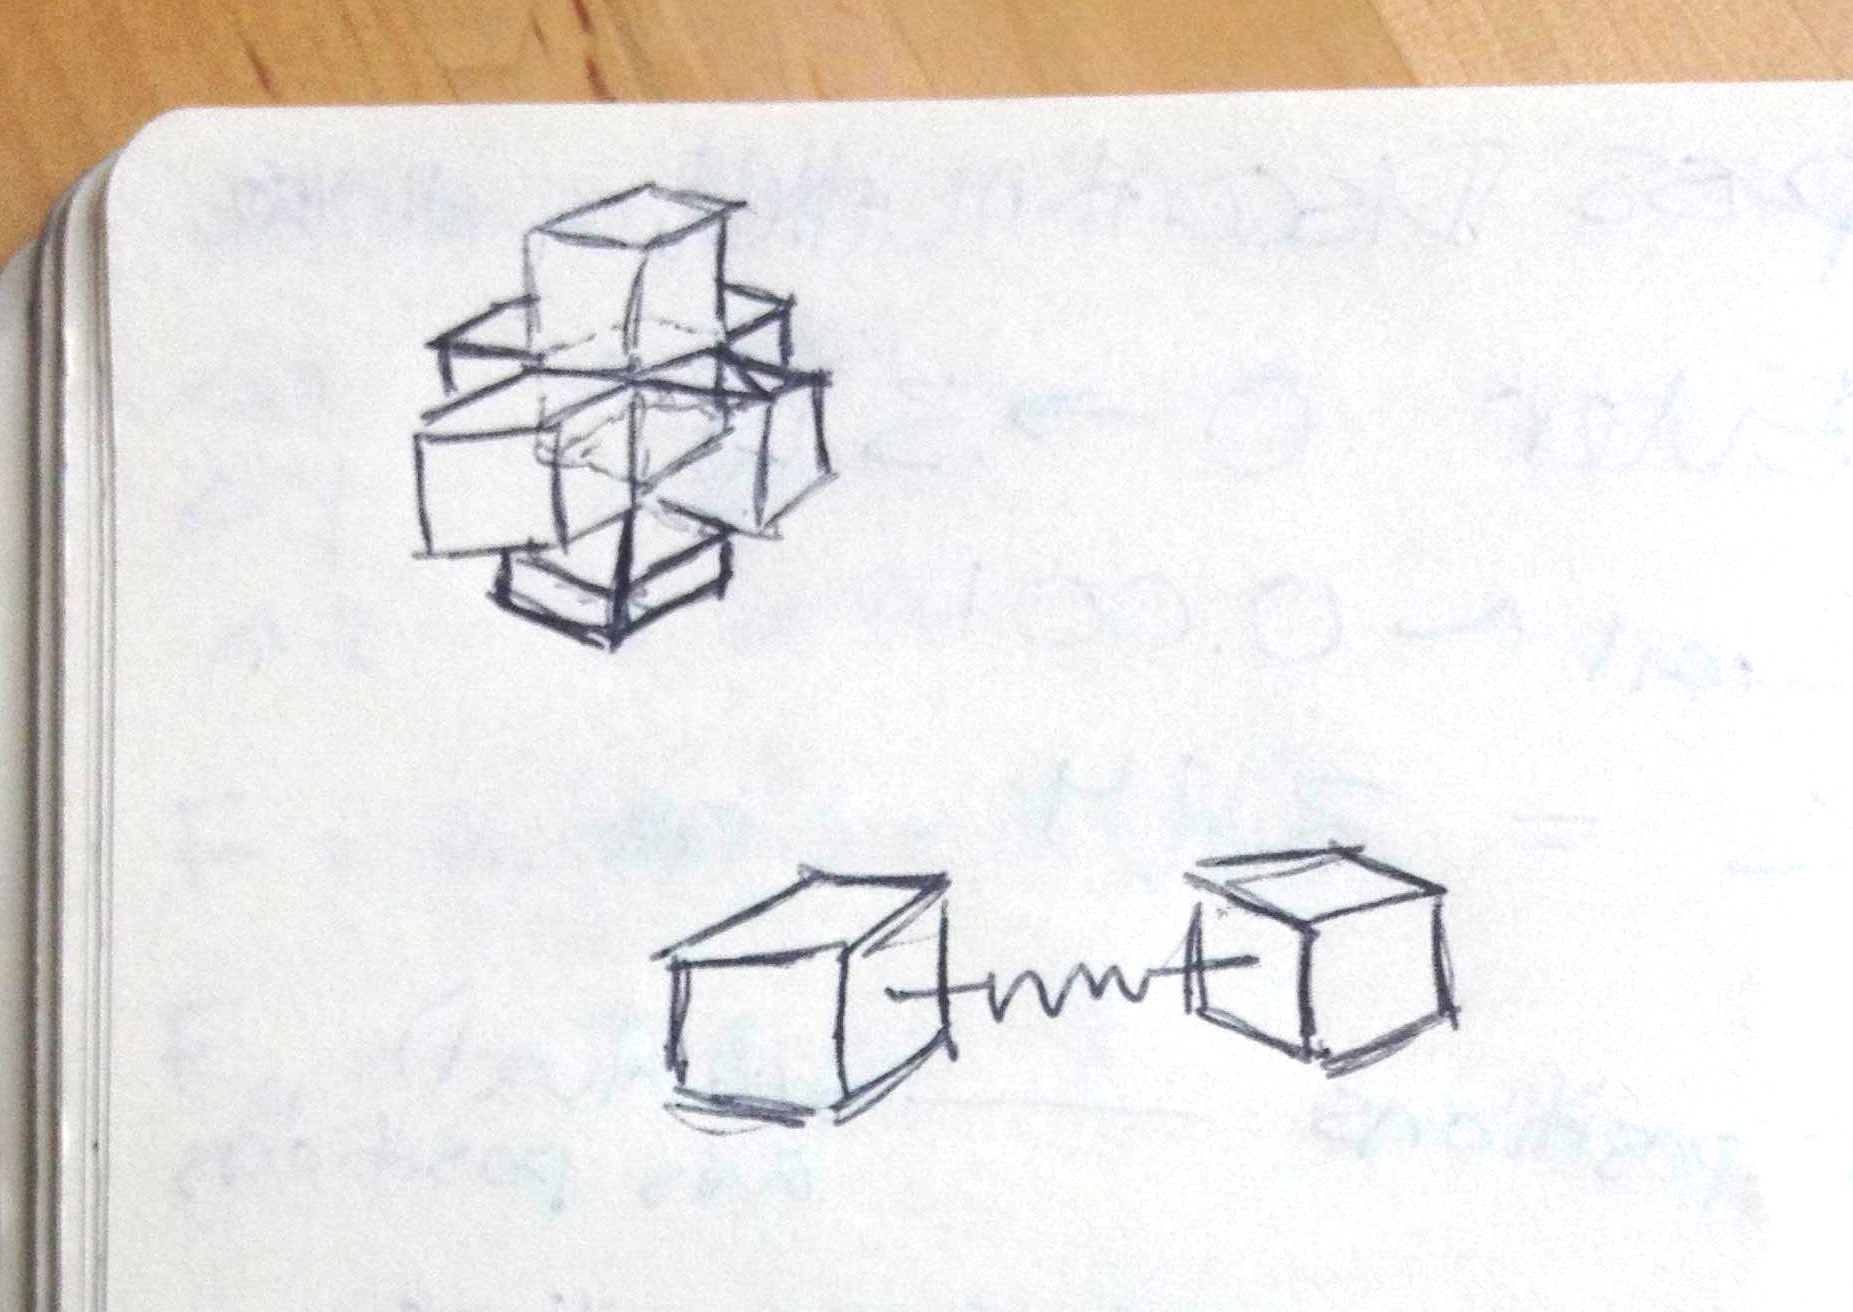
\includegraphics[width=\linewidth]{helloWorldLocalInteraction.png}
%  \caption{REPLACE THIS Each cell is face-connected to its six local neighbors \textbf{(A)}.  Interaction between neighbors is modeled with springs and dampers constraining translational and rotational motion \textbf{(B)}.}
%  \label{fig: helloWorldLocalInteraction}
%\end{figure}
%
%%To understand how the translational spring forces were calculated between two adjacent cells, consider the 2D case illustrated in Fig \ref{fig: helloWorldSpringSetup}.  The cells are attached by a spring with nominal length $\ell$.  Under displacement $\Delta x$ and $\Delta y$, the distance vector from cell A to cell B is given by $\vec{D}$.  Then $\Delta \ell$, the displacement of the spring from its nominal length, is given by:\\
%%
%%\[ \Delta \ell = \| D\| - \ell\]
%%
%%The force, $\vec{f}_{AB}$, exerted on cell A by a spring with stiffness $k$ is oriented in the same direction as $\vec{D}$:
%%
%%\[ \vec{f}_{AB} =  k (\hat{D} \Delta \ell) = k\hat{D} (\|D\| - \ell)\]
%%
%%An equal and opposite force, $\vec{f}_{BA}$, is applied to cell B by the spring:
%%
%%\[ \vec{f}_{BA} = -k\hat{D} (\|D\| - \ell)\]
%%
%%\begin{figure}
%%  \includegraphics[width=\linewidth]{helloWorldSpringSetup.png}
%%  \caption{REPLACE THIS Cubes A and B connected by spring with nominal length $\ell$ \textbf{(A)}.  The cells are displaced by $\Delta x$ and $\Delta y$ \textbf{(B)}. Spring displacement $\Delta \ell$ along $\vec{D}$ \textbf{( C )}.  $\vec{f}_{AB}$ and $\vec{f}_{BA}$ are the resulting translational spring forces applied to cells A and B, respectively \textbf{(D)}.  Larger translational displacements between neighboring cells increase the amplitude of spring forces \textbf{(E)}.}
%%  \label{fig: helloWorldSpringSetup}
%%\end{figure}
%
%To understand how the translational forces were calculated between two adjacent cells, consider the 2D case illustrated in Fig \ref{fig: helloWorldSpringSetup}.  The cells are attached to each other with nominal displacement $\vec{\ell}$ from the center of cell A to the center of cell B.  If we model a two dimensional spring damper system connecting the cells, then the force applied to cell A by cell B under additional displacement $\Delta x$ and $\Delta y$ is given by:
%
%\[ \vec{f}_{AB} =   k\left[ \begin{array}{ccc}
%\Delta x \\
%\Delta y \end{array} \right] - d 
%\left[ \begin{array}{ccc}
%v_x\\
%v_y\end{array} \right] 
% \]
%
%where k is a spring stiffness, d is a damping coefficient, and $v$ is the velocity of cell A relative to cell B.  This equation is trivially extended to the three dimensional case:\\
%
%\[ \vec{f}_{AB} =   k\left[ \begin{array}{ccc}
%\Delta x \\
%\Delta y\\
%\Delta z \end{array} \right] - d 
%\left[ \begin{array}{ccc}
%v_x\\
%v_y\\
%v_z\end{array} \right] 
% \]
%
%\begin{figure}
%  \includegraphics[width=\linewidth]{helloWorldSpringSetup.png}
%  \caption{REPLACE THIS Adjacent cells A and B connected with nominal displacement $\vec{\ell}$ \textbf{(A)}.  The cells are additionally displaced by $\Delta x$ and $\Delta y$ \textbf{(B)}. $\vec{f}_{AB}$ and $\vec{f}_{BA}$ are the resulting translational spring-damper forces applied to cells A and B, respectively \textbf{( C )}.}
%  \label{fig: helloWorldSpringSetup}
%\end{figure}
%
%
%The stiffness $k$ and damping coefficient $d$ of the springs and dampers are determined from the material properties of the two cells.  In the case that the two cells have different stiffnesses, a composite stiffness is calculated according to:
%
%\[ k = \frac{2k_Ak_B}{k_A + k_B} \]
%
%which is equivalent to two springs of half length in series.  Similarly, a composite damping coefficient is calculated by:\\
%
%\[ d = \frac{2d_Ad_B}{d_A + d_B} \]
%
%In addition to $\vec{f}_{AB}$, an equal and opposite force, $\vec{f}_{BA}$, is applied to cell B by the spring damper system (Fig \ref{fig: helloWorldSpringSetup} C):
%
%\[ \vec{f}_{BA} =  -\vec{f}_{AB}\]
%
%In addition to translational forces, neighboring cells apply torques to each other.  These torques result in rotational motion of a cell about its center of mass.  More on that soon.
%
%%\begin{figure}
%%  \includegraphics[width=\linewidth]{helloWorldSpringSetup.png}
%%  \caption{REPLACE THIS Cubes A and B connected by spring with nominal displacement $\ell$ \textbf{(A)}.  The cells are further displaced by $\Delta x$ and $\Delta y$ \textbf{(B)}. Spring displacement $\Delta \ell$ along $\vec{D}$ \textbf{�}.  $\vec{f_{AB}}$ is the translational spring resulting force applied to cell A by the spring attached to cell B, force of gravity, $f_g$, also indicated \textbf{(D)}.}
%%  \label{fig: helloWorldSpringRotSetup}
%%\end{figure}
%
%
\section{Rotational Forces}

\begin{figure}
  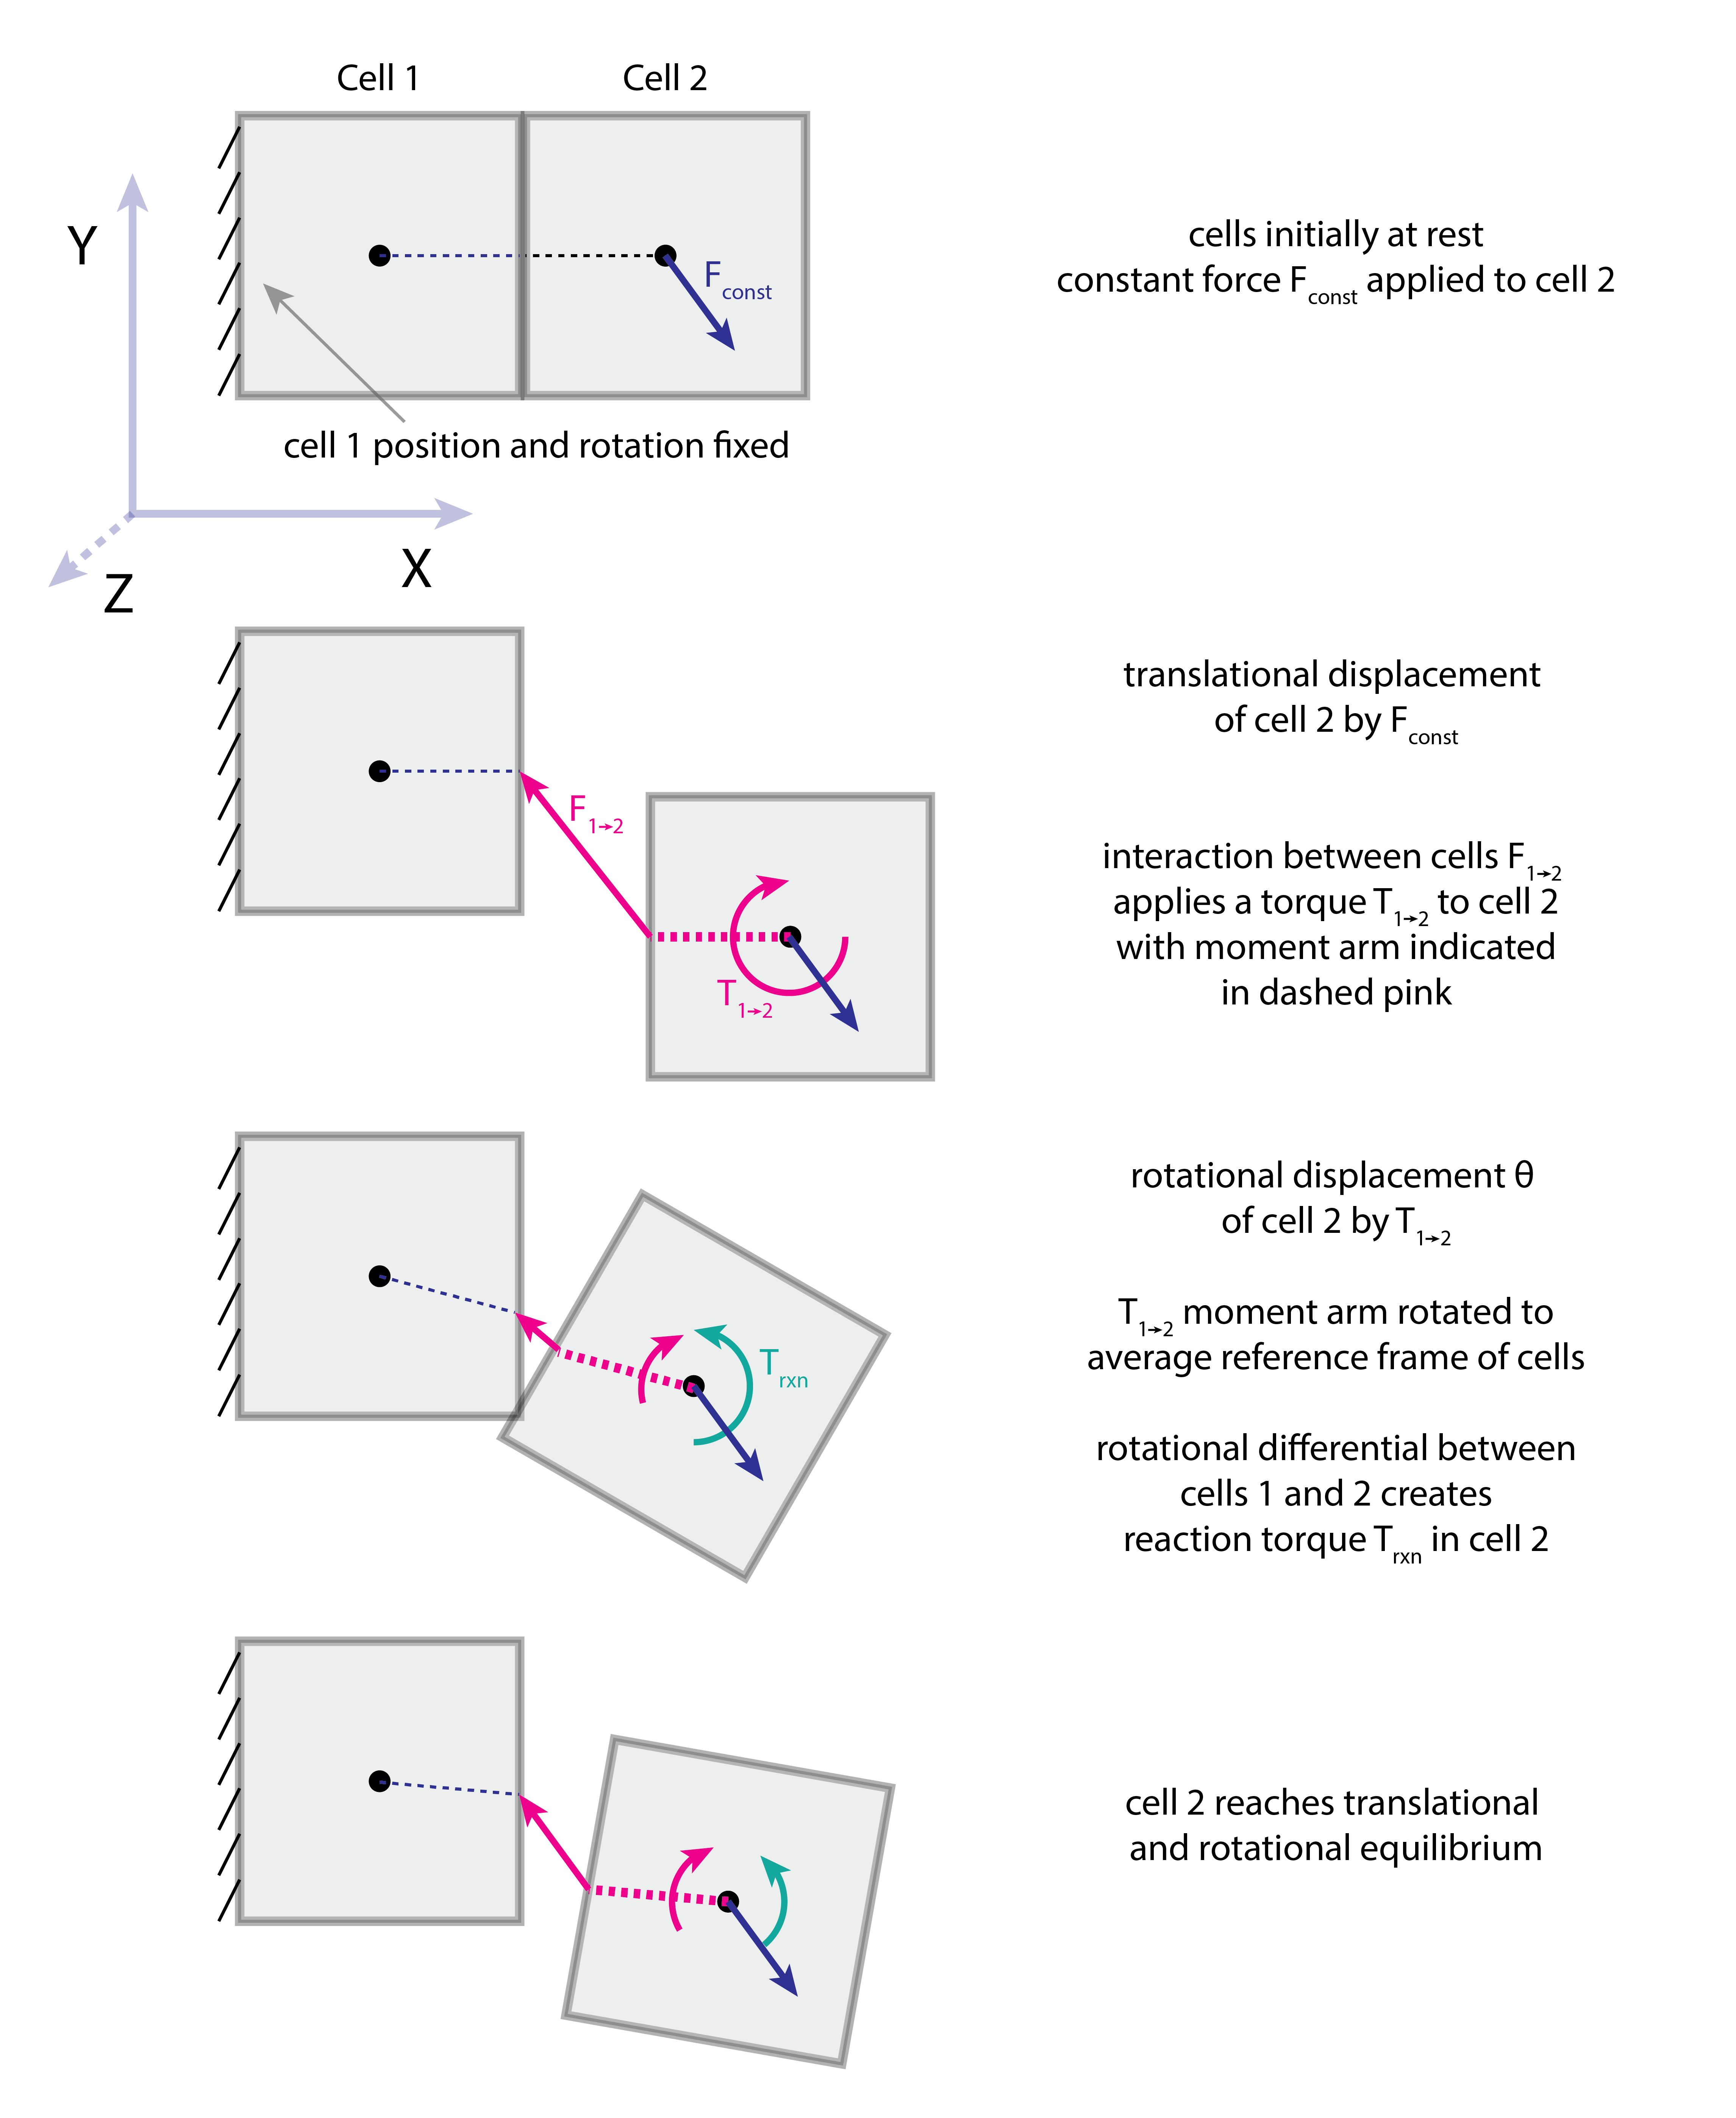
\includegraphics[width=\linewidth]{rotationalSim.png}
  \caption{rotationalSim}
  \label{fig:rotationalSim}
\end{figure}

\section{Sources of Error}

\subsection{Numerical Time Integration}

For linear systems, explicit forward time integration can be achieved using a variety of methods, each with associated error and computational cost.  The simplest and most computationally efficient approach is forward Euler:
\[ \vec{v}_{t+1} = \vec{v}_{t} +  \vec{a}_{t}\Delta t\]
\[ \vec{p}_{t+1} = \vec{p}_{t} +  \vec{v}_{t}\Delta t\]

Verlet integration requires storing the previous two position calculations (at time t and t-1) in order to calculate the next position:
\[ \vec{p}_{t+1} = 2\vec{p}_{t} - \vec{p}_{t-1} +  \vec{a}_{t}\Delta t^2\]
\[ \vec{v}_{t+1} = \dfrac{\vec{p}_{t+1} - \vec{p}_{t}}{\Delta t}\]

Higher order methods such as Runge-Kutta (RK4) reduce error further, but require multiple calculations in order to solve for a single time step.

\subsection{Floating Point Operations}

\section{Electronic Simulation}\label{sec:electronicSim}

\section{Hierarchical Simulation}

\section{Performance Speedups}

A faster method of applying quaternions to vectors is given by
\[ t = 2 \left[ \begin{array}{ccc}
q_x\\
q_y\\
q_z
 \end{array} \right] \times v\]
\[ v_{rotated} = v + q_wt +  \left[ \begin{array}{ccc}
q_x\\
q_y\\
q_z
 \end{array} \right] \times t\]
 https://blog.molecular-matters.com/2013/05/24/a-faster-quaternion-vector-multiplication/


%\section{Deviations from Reality}
%
%\subsection{Volume Preservation}
%
%Poisson's ratio $v$
%
%\begin{figure}
%  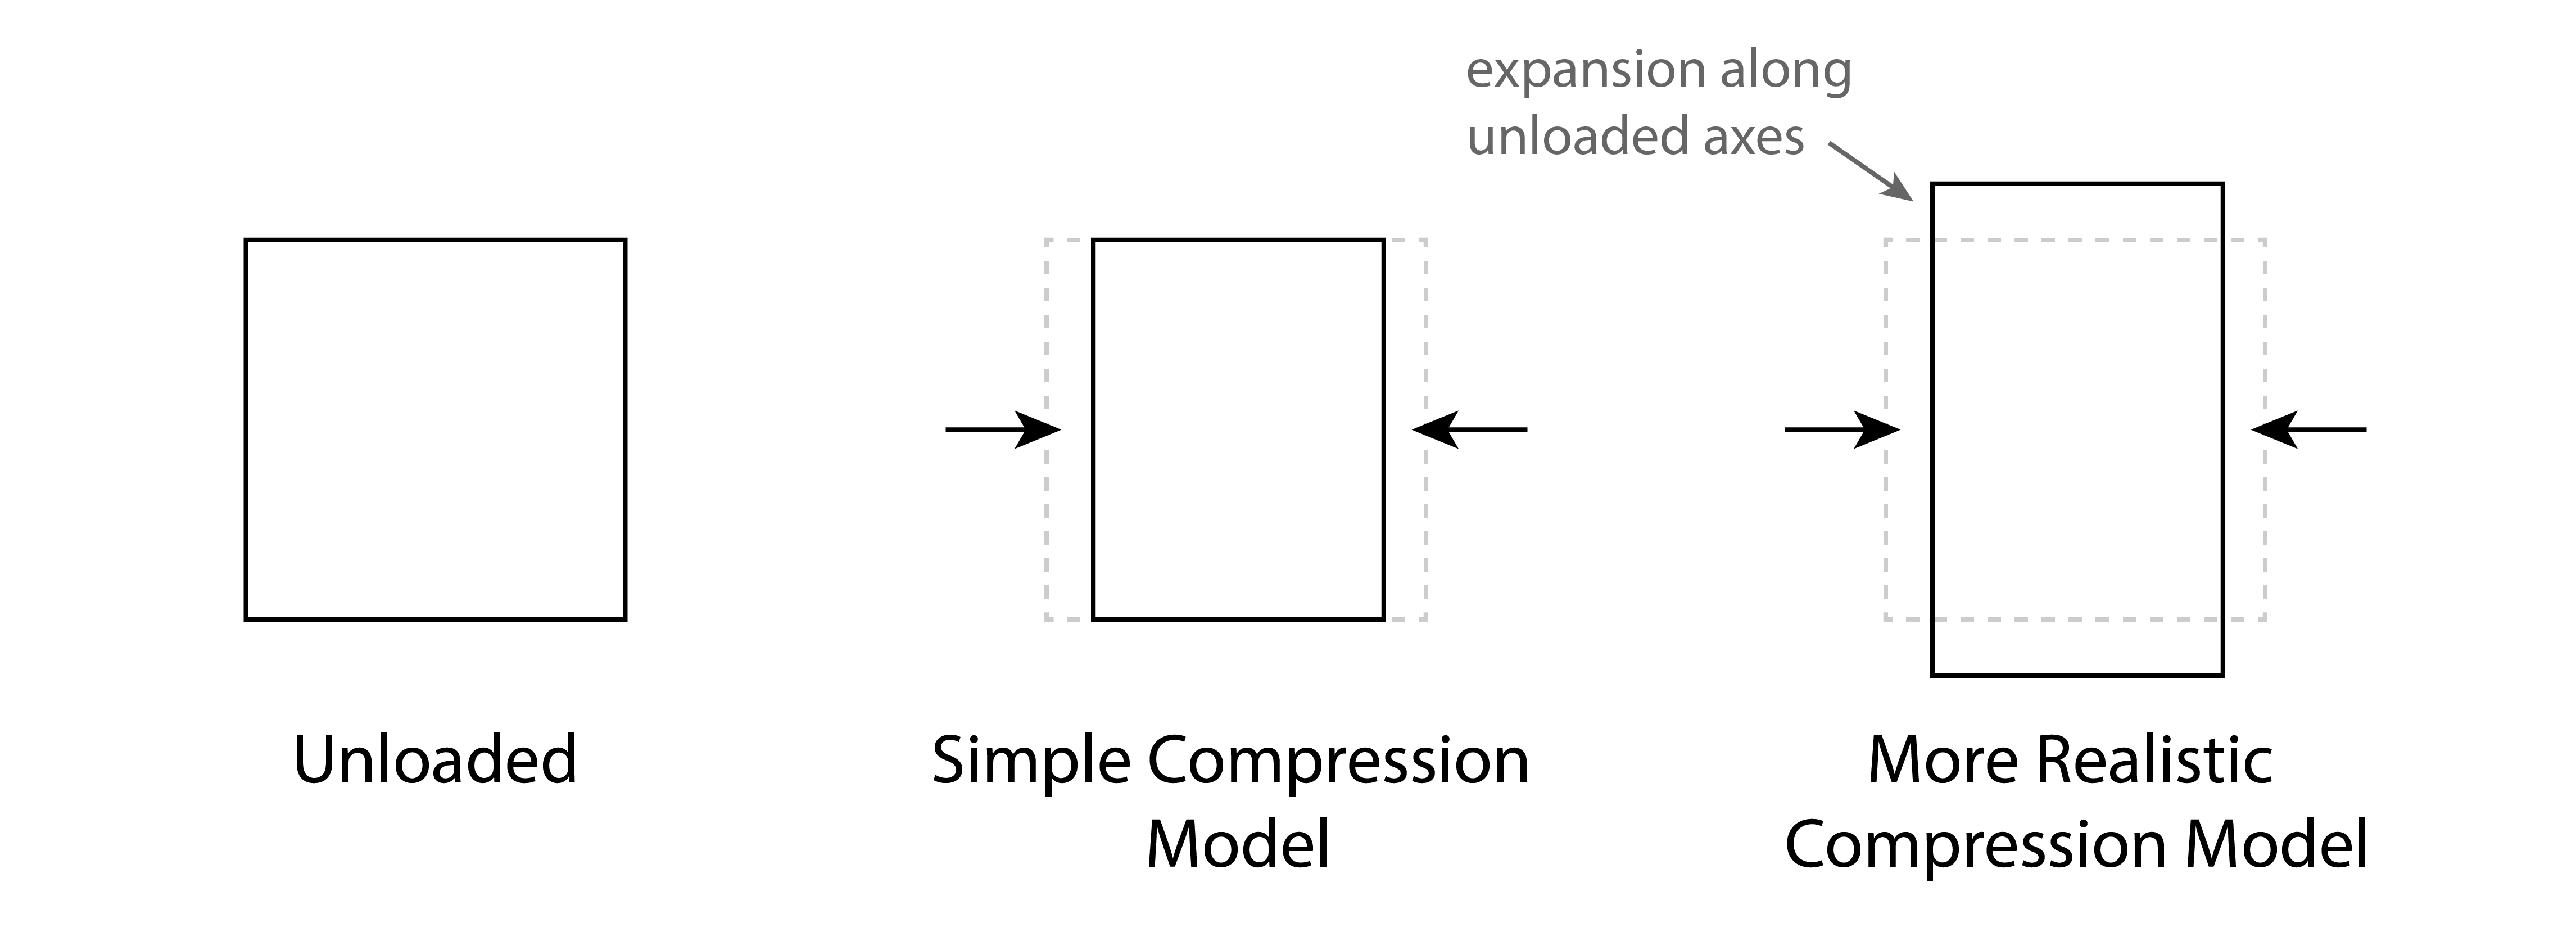
\includegraphics[width=\linewidth]{SolidMechanicsReality.png}
%  \caption{Deviation from reality in simple \textit{function} simulation.  Some coupling between degrees of freedom is expected, for example, compression on one axis will result in expansion along other, unloaded axes.}
%  \label{fig:SolidMechanicsReality}
%\end{figure}
%
%In reality, the degrees of freedom illustrated in Fig \ref{fig:SolidMechanicsDOF} are not completely orthogonal from one another.  For example, compression along one axis of a solid will cause some degree of expansion along the unloaded axes (Fig \ref{fig:SolidMechanicsReality}).  For now, I have ignored these effects.



}

%%% This is an example first chapter.  You should put chapter/appendix that you
%% write into a separate file, and add a line \include{yourfilename} to
%% main.tex, where `yourfilename.tex' is the name of the chapter/appendix file.
%% You can process specific files by typing their names in at the 
%% \files=
%% prompt when you run the file main.tex through LaTeX.

\singlespacing{

\chapter{Implementation}\label{chap:implementation}

(still need to name it)\\

\href{http://git.amandaghassaei.com/KinematicCA/}{TBD} is a 3D CAD and simulation tool, based off the ideas from Chapters \ref{chap:CAD} and \ref{chap:functionSim}.  In this tool, users construct assemblies of functional primitives and simulate their electronic and mechanical behaviors.  This chapter introduces information about the software implementation of TBD.

\section{Javascript/WebGL}

TBD was written in HTML5/JavaScript and currently hosted online.  I chose the web as a development platform for this project because it allows easier access to the code than any other platform.  Though user studies are not a component of this work, there is a long history of communities of users building things in sandbox environments that surpass anything the developers were able to imagine.  There is a lot of talent beyond the immediate neighborhood of CBA, and I'd like to try to make this codebase accessible to anyone interested in exploring the design space around digital materials.\\

The web app was written with the following dependencies:
\begin{itemize}
\setlength\itemsep{0em}
\item \href{http://threejs.org/}{Three.js} is a library containing lots of useful classes for interacting with WebGL without getting bogged down in the details or sacrificing too much in performance.
\item \href{http://requirejs.org/}{RequireJS} is a framework for asynchronously loading JavaScript modules and dependencies.
\item \href{http://backbonejs.org/}{Backbone.js} is a framework for managing UI events and giving structure to complex, interactive applications.
\item \href{https://jquery.com/}{JQuery} is a library that handles interactions between HTML and Javascript and helps maintain cross browser support of UI elements.
\item \href{http://underscorejs.org/}{Underscore} is a library with lots of useful functions for dealing with arrays and JavaScript objects.  Underscore also provides templating for Backbone.
\end{itemize}

\begin{figure}
  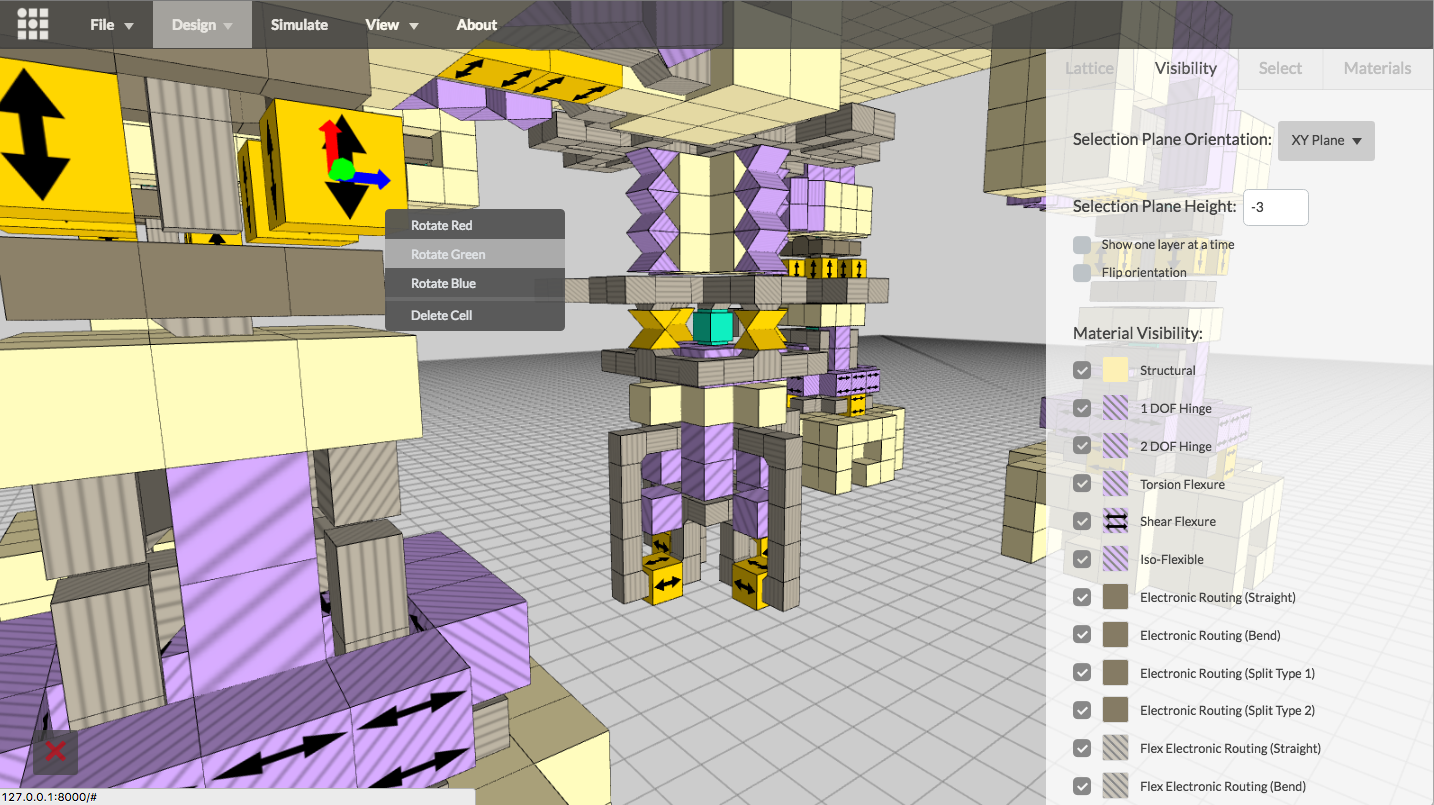
\includegraphics[width=\linewidth]{rotationGUI.png}
  \caption{A schematic diagram of a robotic ``pick and place'' in TBD.  Cell rotation GUI allows anisotropic cells to be oriented in any direction.}
  \label{fig:rotationGUI}
\end{figure}

\begin{figure}
  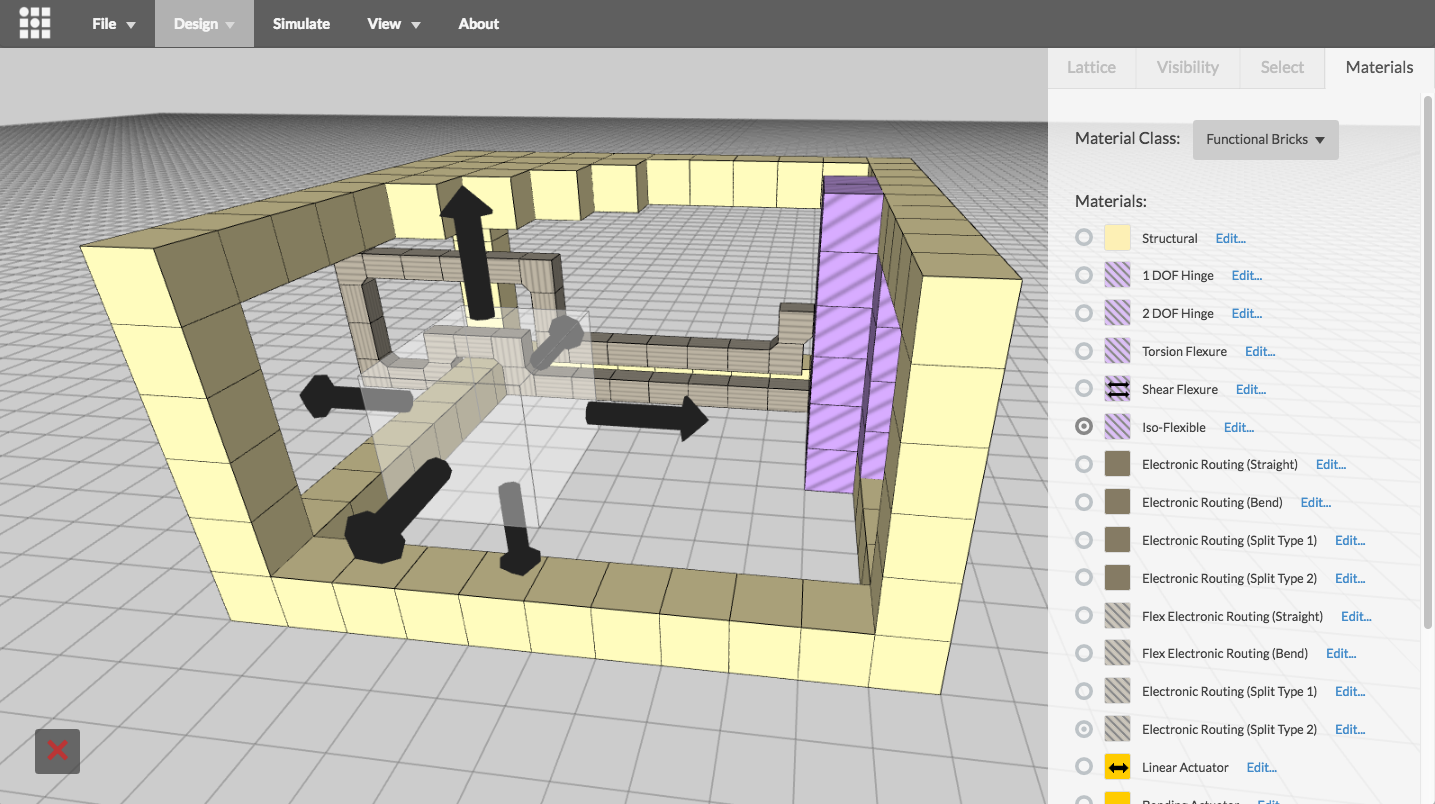
\includegraphics[width=\linewidth]{selectiontoolGUI.png}
  \caption{3D selection tool allows for bulk cell additions and removals, and cloning or mirroring existing geometry.}
  \label{fig:selectiontoolGUI}
\end{figure}

\begin{figure}
  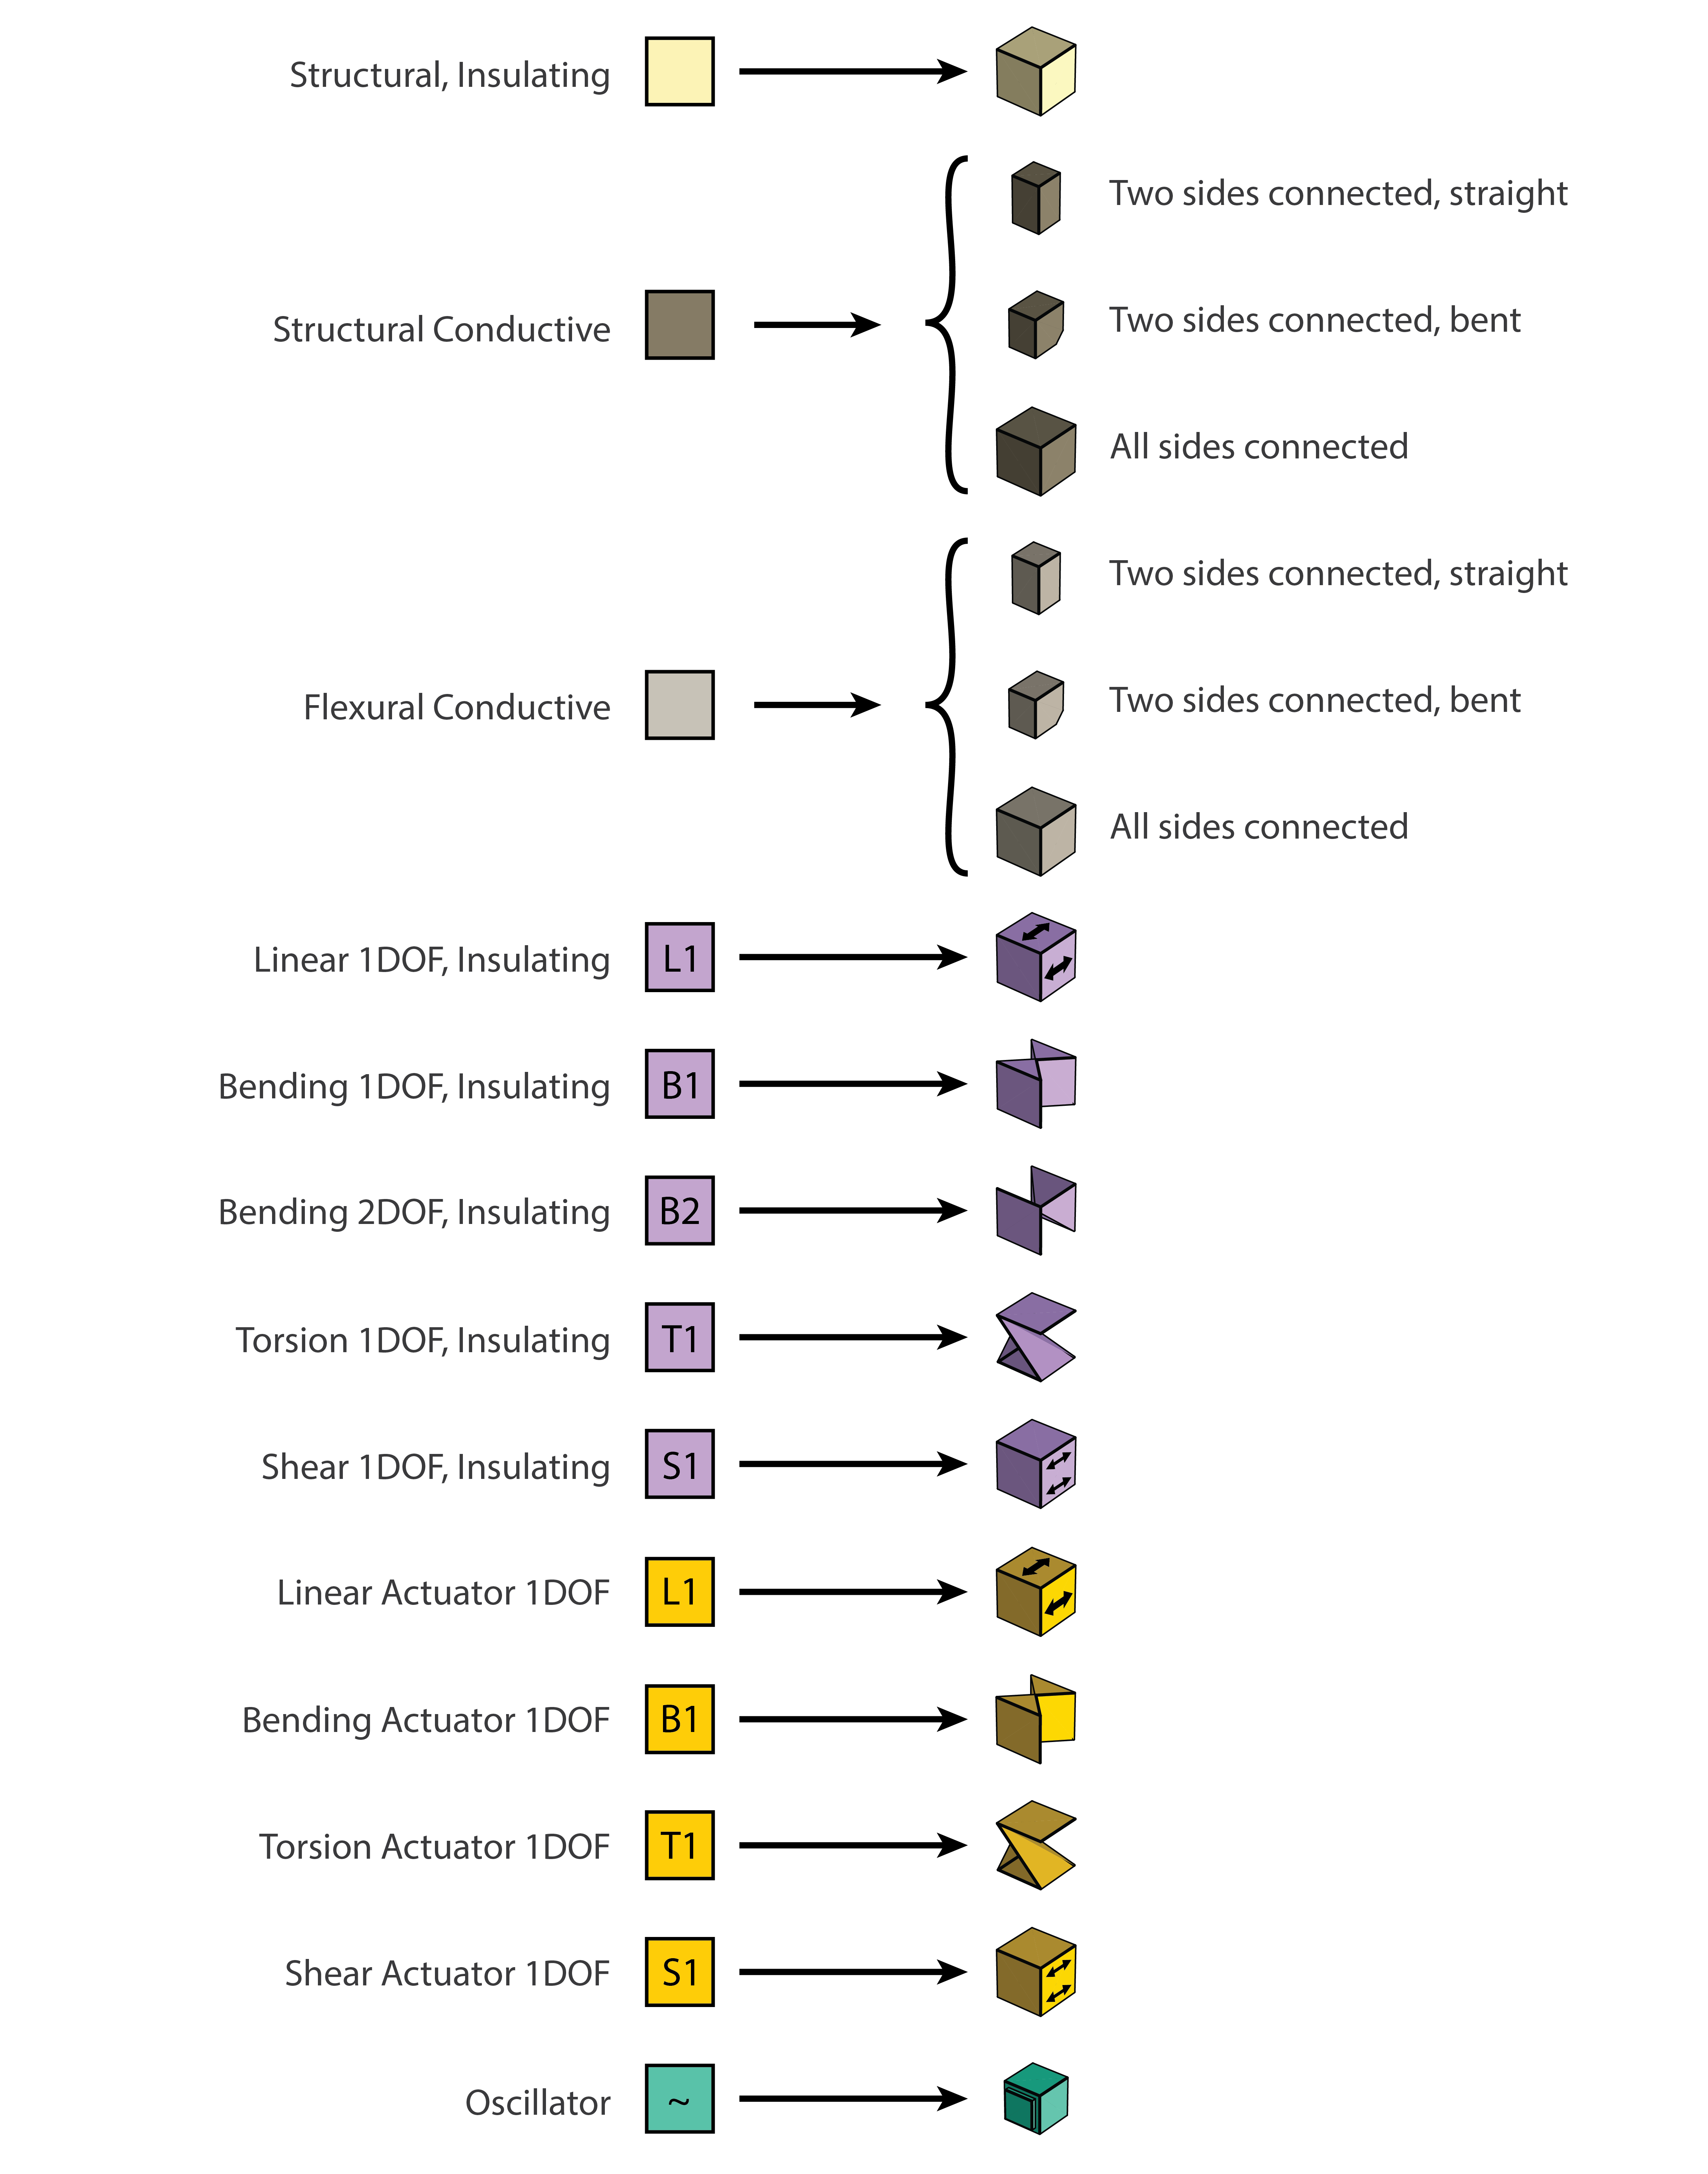
\includegraphics[width=\linewidth]{cellMeshes.png}
  \caption{Meshes and textures used to represent different material types and convey the orientation of cell anisotropy.}
  \label{fig:cellMeshes}
\end{figure}

\section{GUI}

TBD borrows most of its GUI from DMDesign (Chapter \ref{chap:CAD}), with a few exceptions.  A cell rotation interface (Figure \ref{fig:rotationGUI}) allows users to rotate cells in 3D, so anisotropic cells may be oriented in any direction.  Absolute cell orientations are saved as JSON when the assembly is saved.  A 3D selection tool allows users to select large rectangular regions of space to fill with material, cut away material, and clone or mirror an existing structure into another region (Figure \ref{fig:selectiontoolGUI}).\\

\begin{figure}
  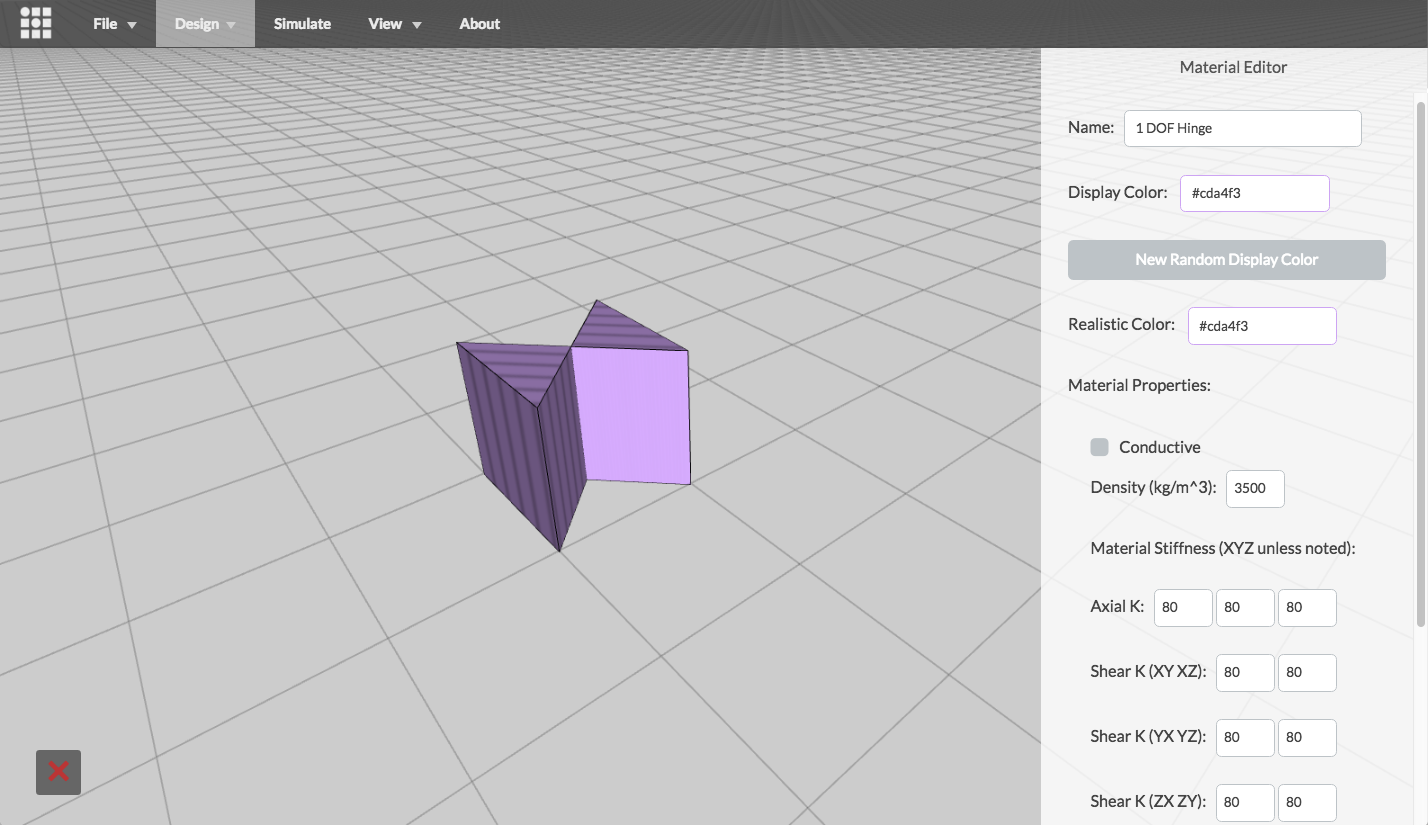
\includegraphics[width=\linewidth]{materialEditor.png}
  \caption{Material editor interface for a 1DOF bending flexure.  All 15 stiffness and damping constants may be edited, along with density and conductivity.}
  \label{fig:materialEditor}
\end{figure}

Anisotropic cells in TBD are represented graphically with special meshes, illustrated in Figure \ref{fig:cellMeshes}.  Some cells (e.g. the straight and bent conducting cells) appear to occupy a smaller volume than other cells, but this is meant only as a visualization of their properties.  All cells fill the same volume and are joined mechanically with six face-connected neighbors.  Isotropic and anisotropic materials may be edited or defined through the material editor interface (Figure \ref{fig:materialEditor}).\\

\section{GPU Programming}

%JavaScript is loosely typed and therefore not an especially fast language out of the box.  Storing large datasets in typed arrays helps to speed up array operations and access at runtime \cite{Network}.  Most modern web browsers support Just In Time (JIT) compilation of JavaScript code, which helps make it more competitive with compiled languages.    Still, it tends to run slower than native C++.\\

\begin{figure}
  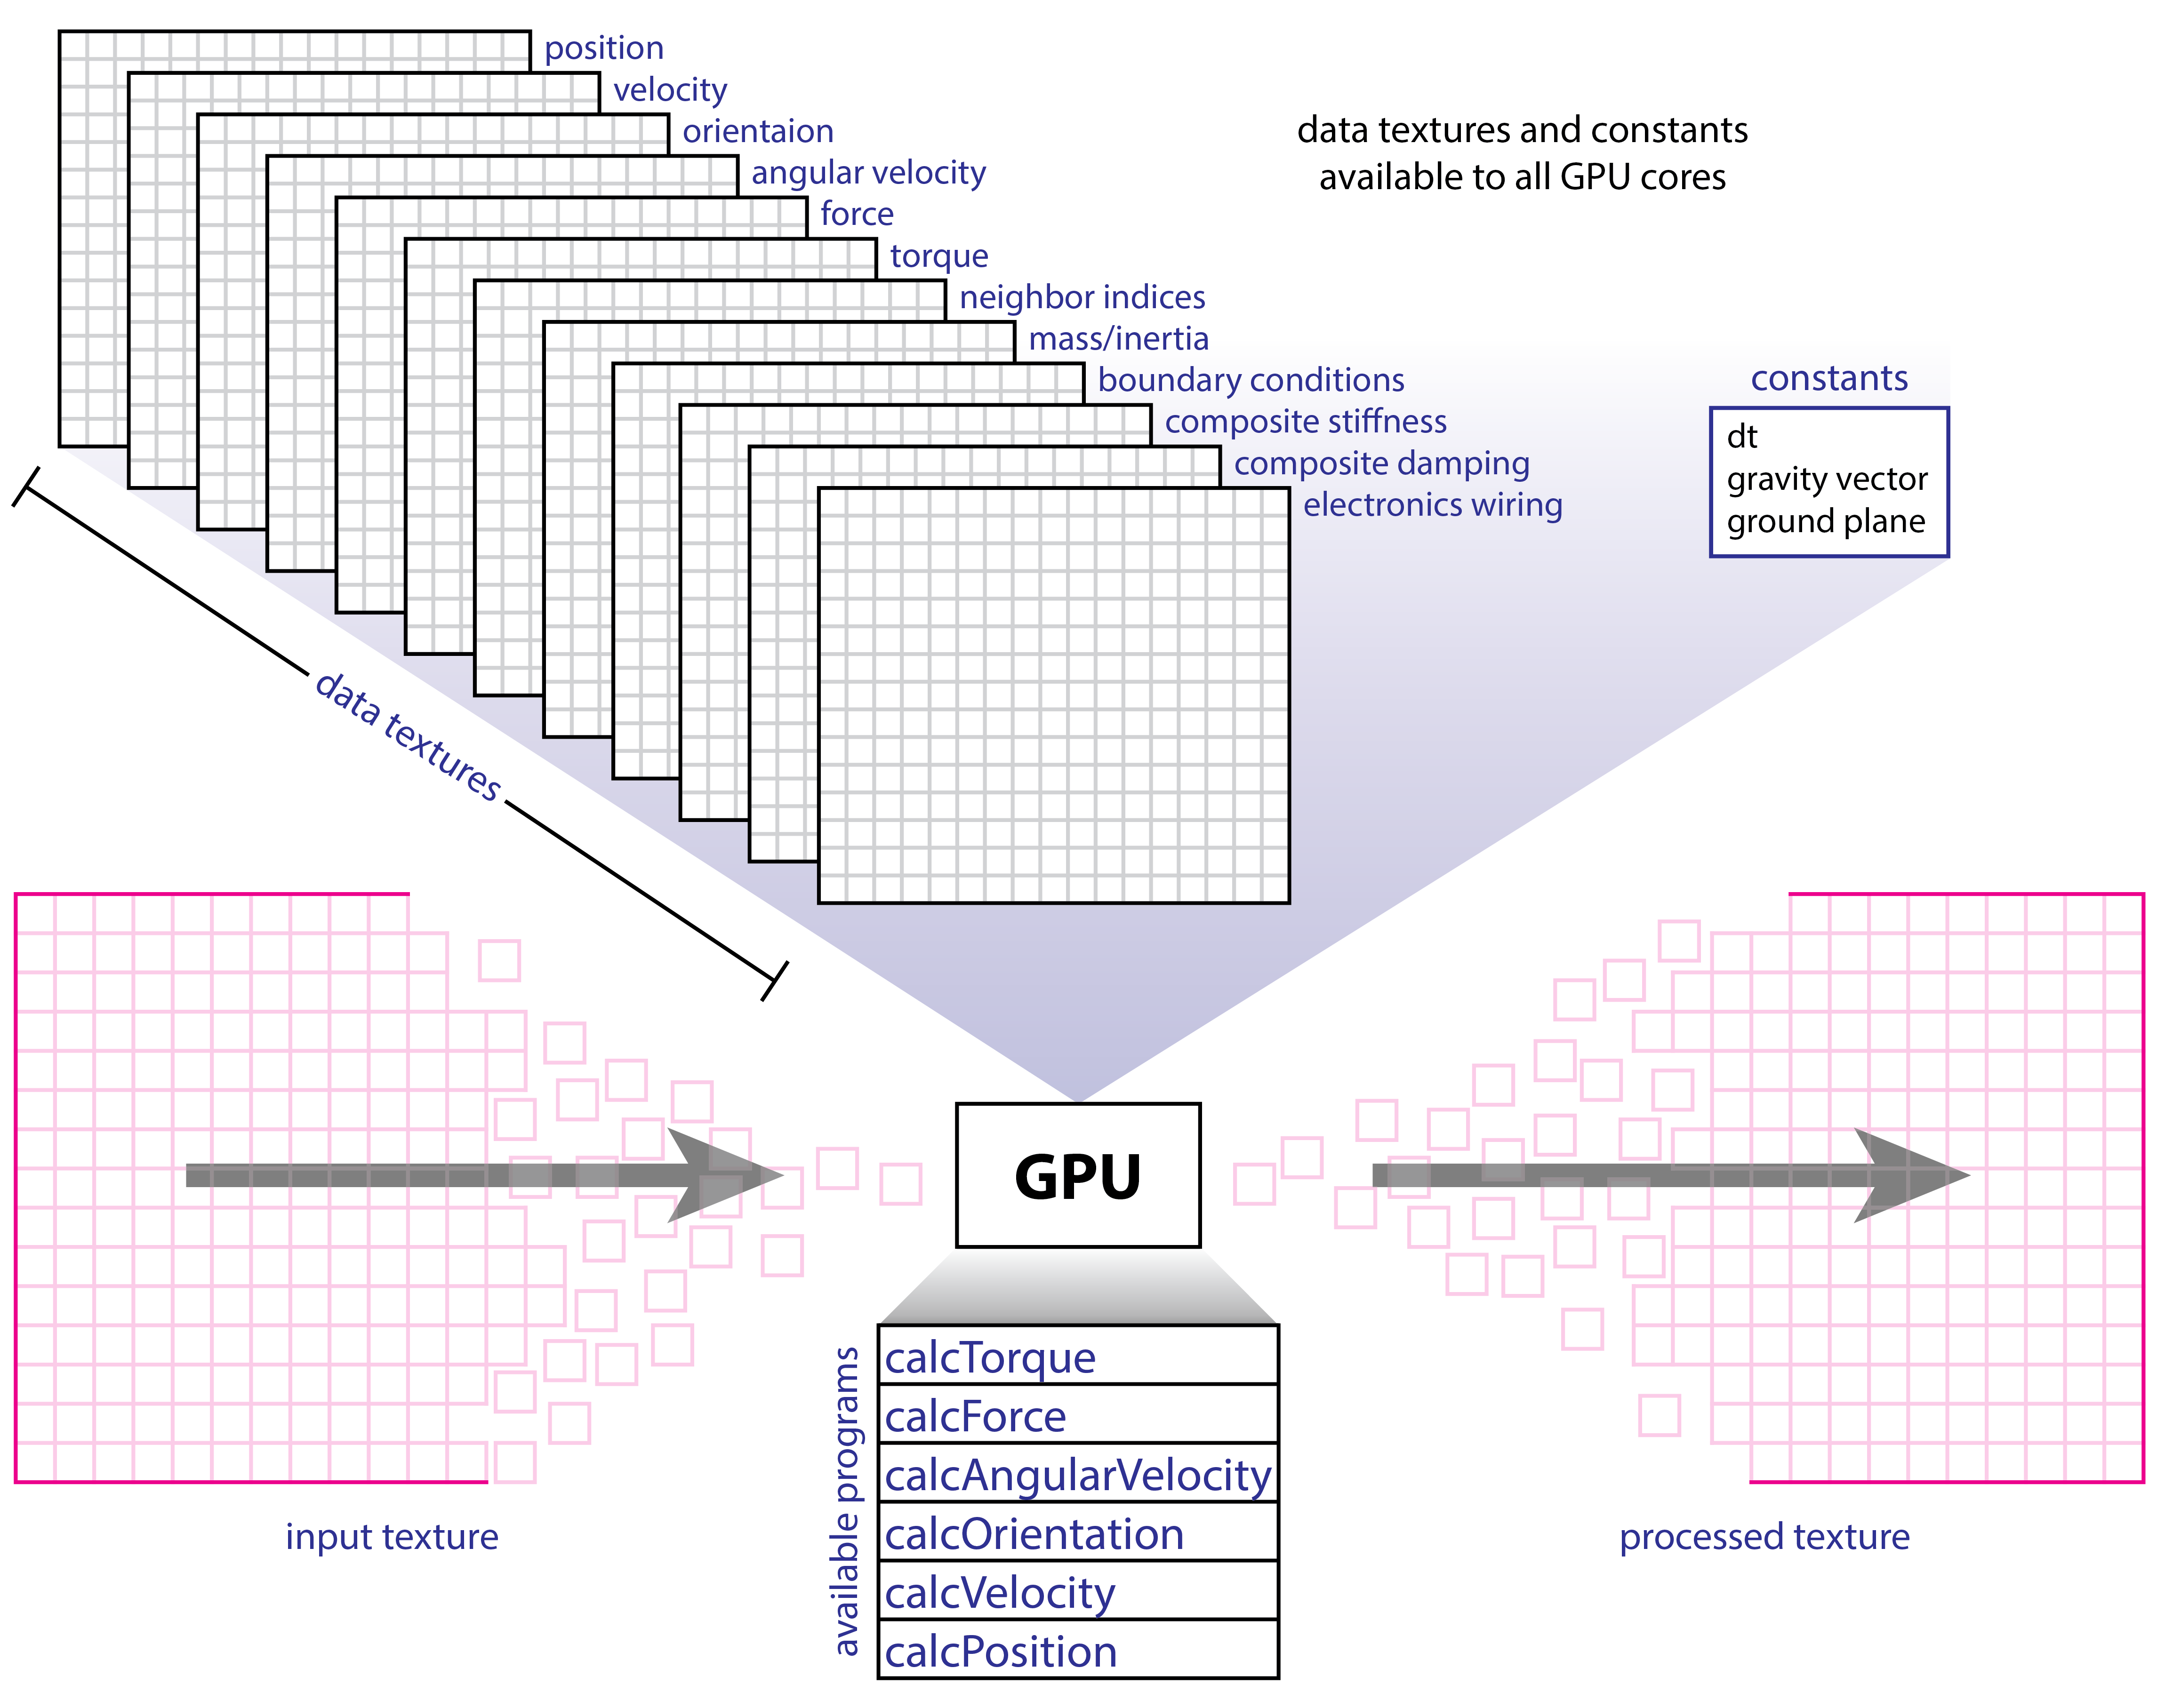
\includegraphics[width=\linewidth]{gpuprogramming.png}
  \caption{Schematic diagram of GPU programming in TBD.  2D data textures store the current state of the cells, lookup tables for neighboring indices, and precomputed composite stiffness and damping constants.  These data textures as well as some global constants are passed into the GPU and are available to all cores.  An input texure buffer is sent into the GPU, split up into RGBA pixels, and used to store the output state from each core.  Several pre-compiled programs are available to the GPU, and are called sequentially during each time step of the simulation (with the exception of PackFloatToBytes, a program used to convert a Float32 texture to a uInt8 texture so that position and orientation can be extracted from the GPU for render).}
  \label{fig:gpuprogramming}
\end{figure}

During the development of TBD, typed arrays \cite{Network} were not performant for assemblies larger than $\sim$30 cells (100 time steps forward per render), so I began running the bulk of the mathematical calculations on the GPU.  Figure \ref{fig:gpuprogramming} shows a schematic representation of the GPU programming.\\

At the moment of writing this, mathematical programming on the GPU through the WebGL API is a bit of a hack.  Data is passed in and out of the GPU cores as 2D arrays - RGBA image textures that would normally be used for rendering purposes.  WebGL currently supports reading and writing Int8/16/32, uInt8/16/32 and Float32 textures.  GPU programs are precompiled as \textit{fragment shaders}, processes that are executed by a single core of the GPU to create a single pixel of output texture data.  Each GPU core may access a number of input data textures but may only output one RGBA pixel to an output texture buffer.  During the execution of a fragment shader program, a complete output texture is calculated by the available GPU cores in a highly parallel, pixel-wise process.  A concise reference for the WebGL API is provided by the Khronos Group \cite{Group}.\\

In TBD, cell state and precomputed constants are stored in several data textures (Figure \ref{fig:gpuprogramming}), and the next state of a given cell is evaluated in a single core of the GPU.  It is not possible to fit all necessary updated state variables (position, velocity, orientation, and angular velocity, all in 3D) in a single RGBA pixel.  This means that calculations for a single time step of the physics engine must be split into several, sequential fragment shader programs (Figure \ref{fig:gpuprogramming}).\\

After moving the simulation forward by some number of time steps, position and orientation information is passed out of the GPU to the main thread for a render call.  Unfortunately, at this time only uInt8 textures may be transferred from the GPU to the CPU.  An additional fragment shader program called ``PackToBytes'' converts the Float32 arrays storing position and orientation into uInt8 arrays, where each float in the original array is converted to four uInt8's.  The process of transferring data from the GPU to the CPU is expensive, and in the fullness of time, could be avoided completely.  TBD is still very much under development and is not ready for these types of low level optimizations yet, but it is something to keep in mind in the following months.\\

Computing in the GPU speeds up the code significatly, but also creates some hardware dependencies that would not have otherwise been present.  For example, some GPUs have a hard limit of 8 textures that can be loaded into memory at a time.  In case of compatibility issues, a backup typed array implementation may be used at the expense of performance.

\section{Other Performance Speedups}

Additional speedups in mathematical operations increase runtime speed of the code.  As demonstrated in Chapter \ref{chap:functionSim}, the math behind the mechanical modeling involves liberal use of quaternions.  An efficient method of applying quaternions to vectors is given below:
\[ t = 2 \left[ \begin{array}{ccc}
q_x\\
q_y\\
q_z
 \end{array} \right] \times v\]
\[ v_{rotated} = v + q_wt +  \left[ \begin{array}{ccc}
q_x\\
q_y\\
q_z
 \end{array} \right] \times t\]
 
 This method uses fewer floating point operations than the standard Hamilton product from equation \ref{eq:hamiltonprod} \cite{Reinalter}.

\section{Instability}

\begin{figure}
  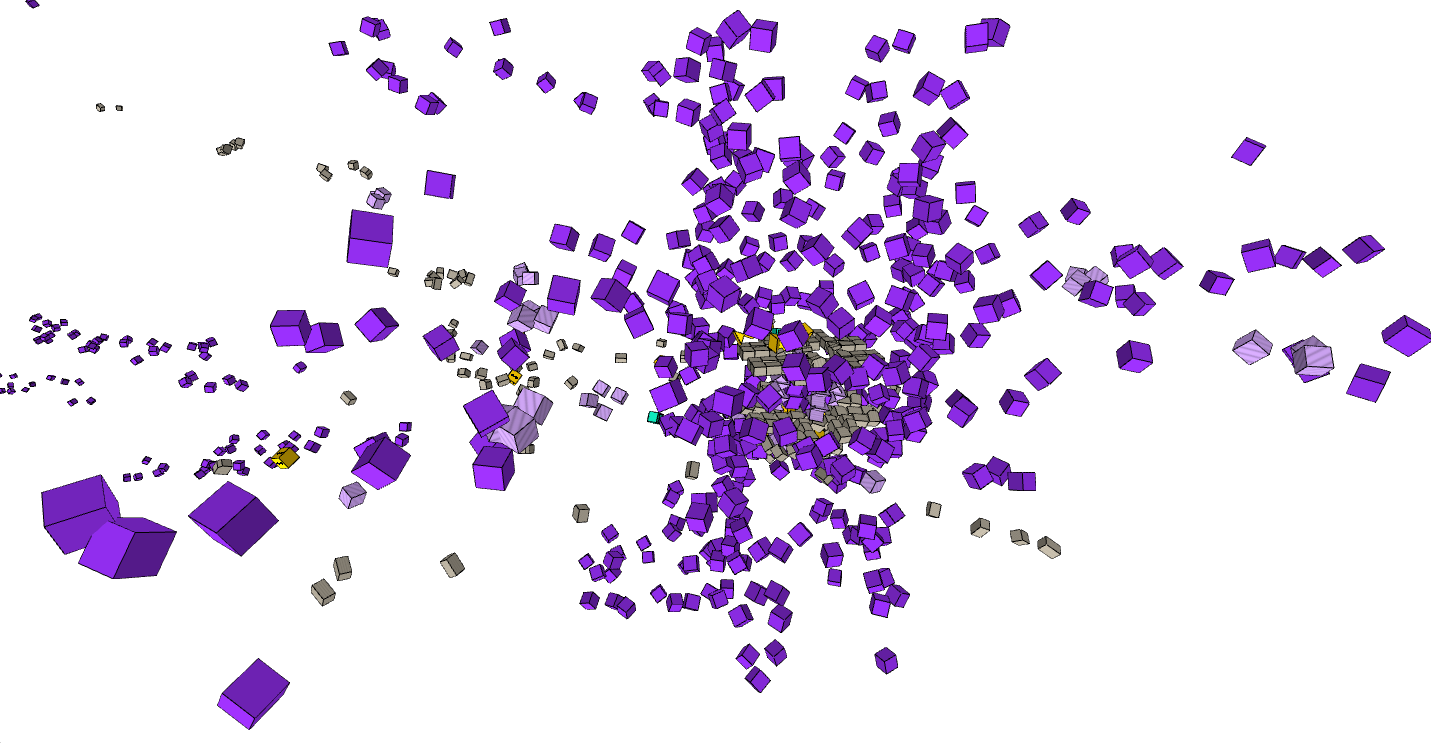
\includegraphics[width=\linewidth]{instability.png}
  \caption{In its current state, TBD is suffering from instability originating in bugs in the simulation code.}
  \label{fig:instability}
\end{figure}

In its current state, TBD is suffering from issues of instability related to bugs in the simulation code.  Additionally, rotational damping has not yet been implemented and its absence tends to throw the system unstable, especially in large, dense assemblies.  This instability tends to look like an explosion (Figure \ref{fig:instability}); as spring systems go unstable they result in massive displacements.  I expect this instability to be resolved in the coming months.

\section{Examples}

\begin{figure}
  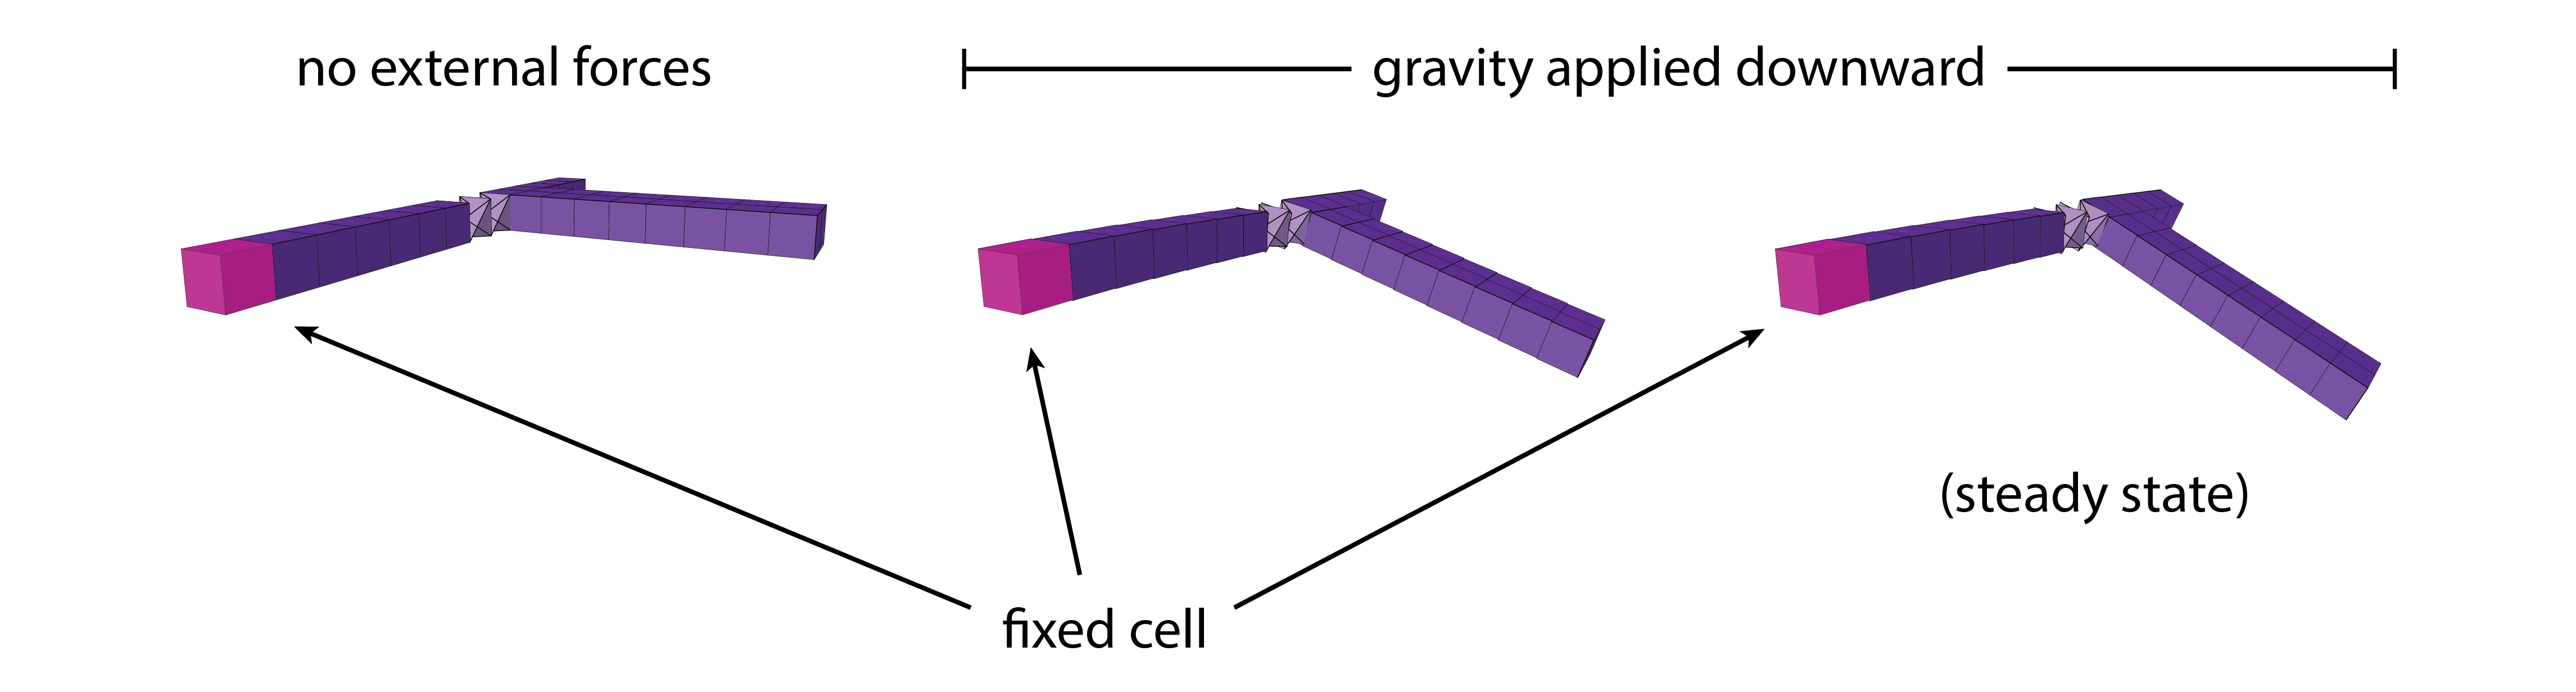
\includegraphics[width=\linewidth]{TorsionSim.png}
  \caption{Simulation of a torsional flexure under a downward force from gravity shows appropriate anisotropic behavior.  Purple are stiff cells, light purple is torsional flexures.  Pink cell is fixed.}
  \label{fig:TorsionSim}
\end{figure}

Due to instability, only certain configurations of parts are currently happy in TBD.  One example is a torsional flexure shown in Figure \ref{fig:TorsionSim}.  An older version of the TBD engine lacked a complete model of torsional and bending stiffness, but tended to be much more stable than the current state of development.  Several examples of simple robotic elements were constructed within this older version of the physics engine (Figures \ref{fig:beambending} through \ref{fig:undulating}).

\begin{figure}
  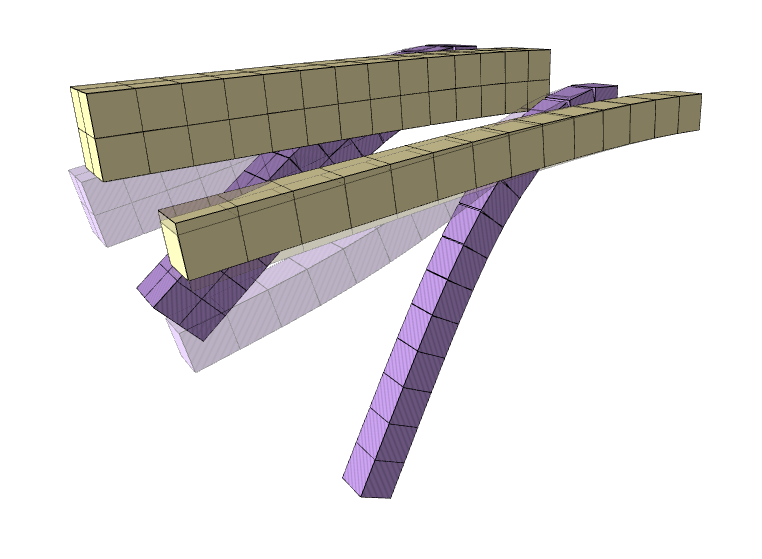
\includegraphics[width=\linewidth]{beambending.png}
  \caption{Beam bending simulation sets one end fixed and allows the rest to deform under gravity.  Both material types shown are isotropic: white material is stiffer than purple.}
  \label{fig:beambending}
\end{figure}

\begin{figure}
  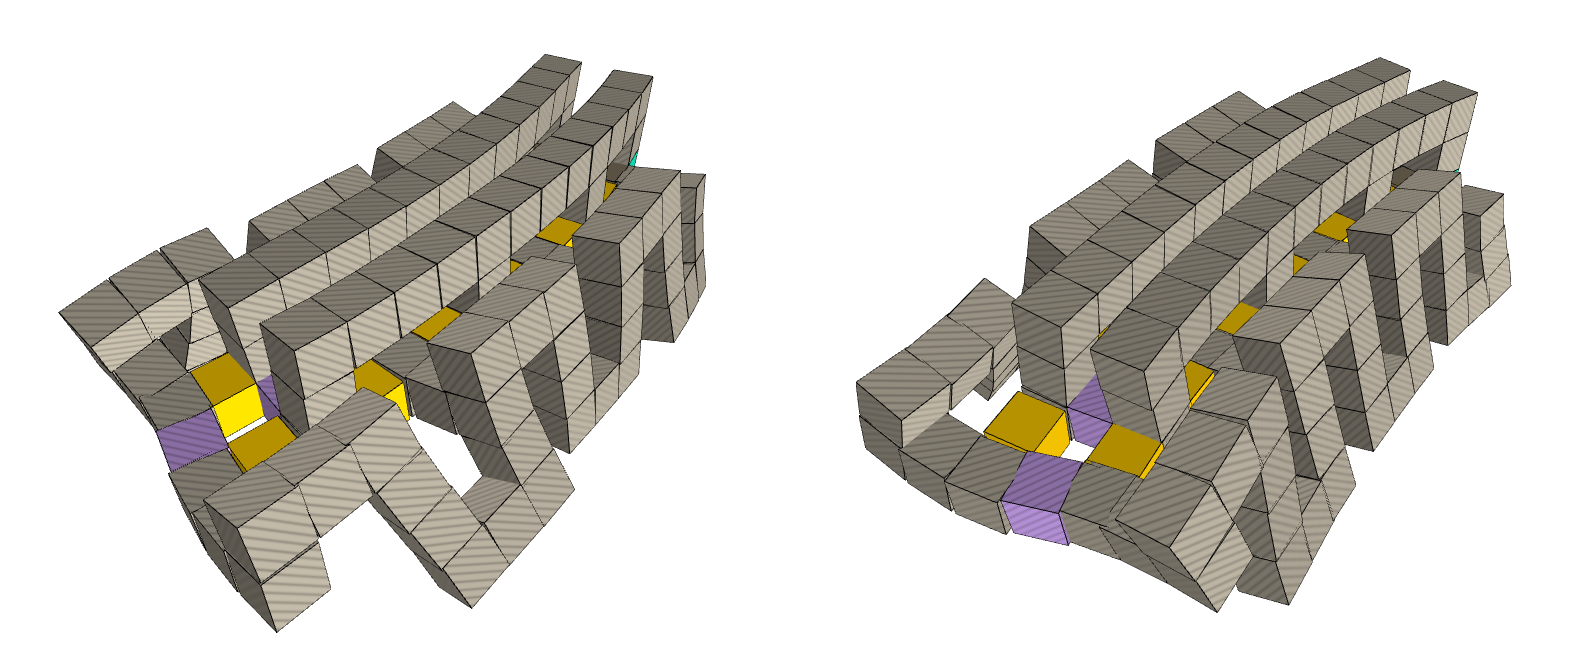
\includegraphics[width=\linewidth]{bendy.png}
  \caption{A bending structure made from two stacks of linear actuators driven out of phase from each other.}
  \label{fig:bendy}
\end{figure}

\begin{figure}
  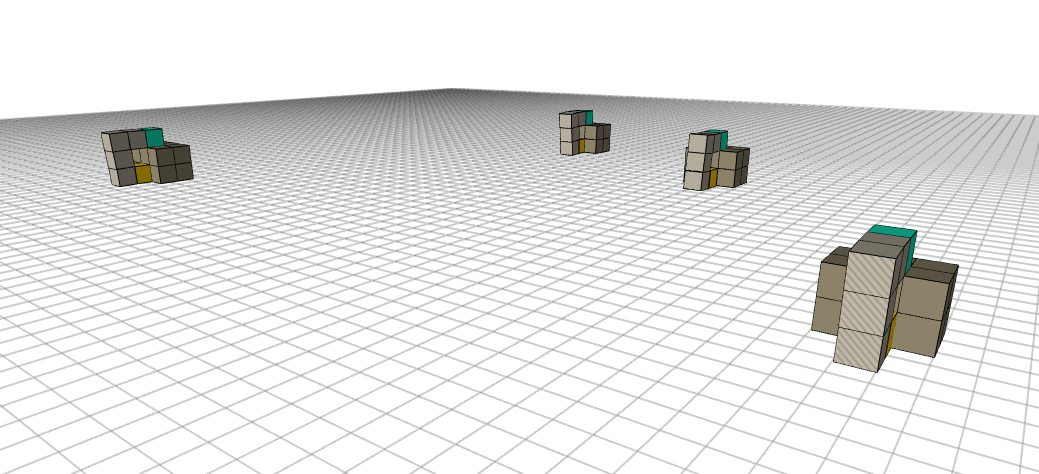
\includegraphics[width=\linewidth]{locomotionsimple.png}
  \caption{Simple locomotion demonstration shows four simple robots, each with a single linear actuator and oscillator.  Differences in speed are due to different oscillator waveforms driving each robot's circuit.  From left to right: sine, square, saw, triangle.}
  \label{fig:locomotionsimple}
\end{figure}

\begin{figure}
  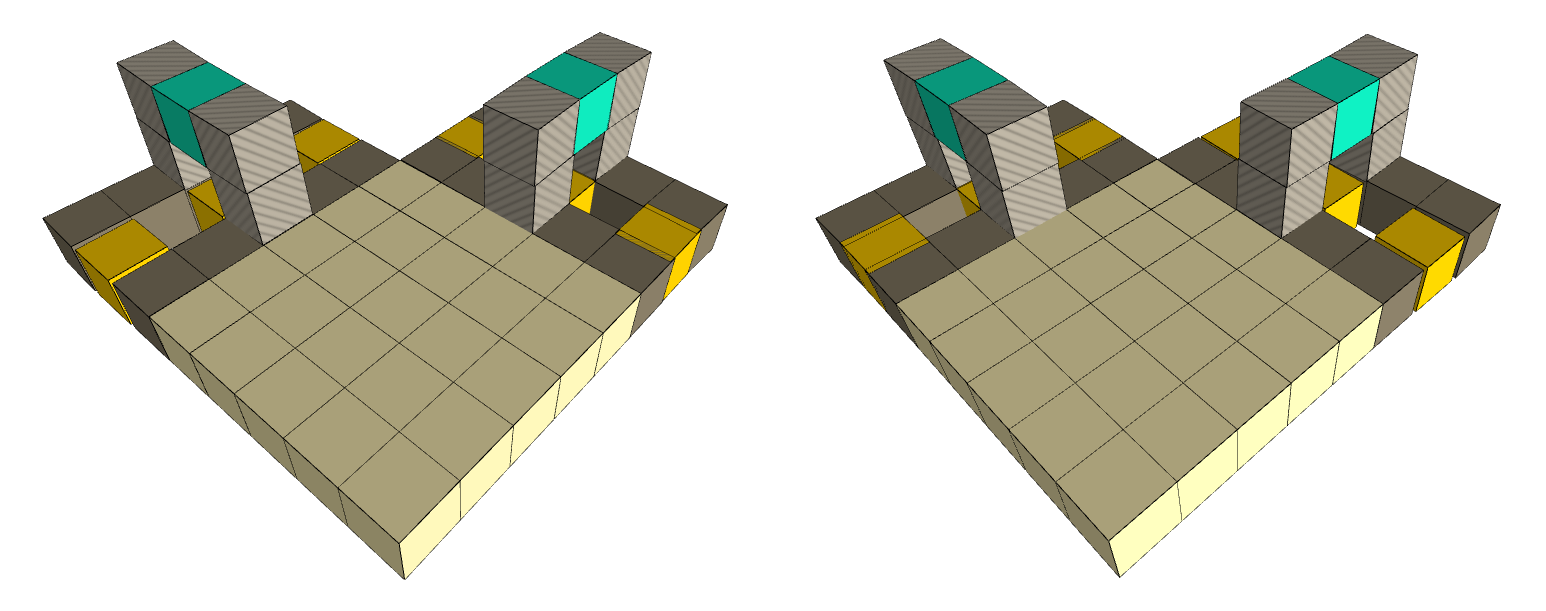
\includegraphics[width=\linewidth]{xystage.png}
  \caption{XY stage driven in a circular motion by two stacks of linear actuators a quarter cycle out of phase from each other.}
  \label{fig:xystage}
\end{figure}

\begin{figure}
  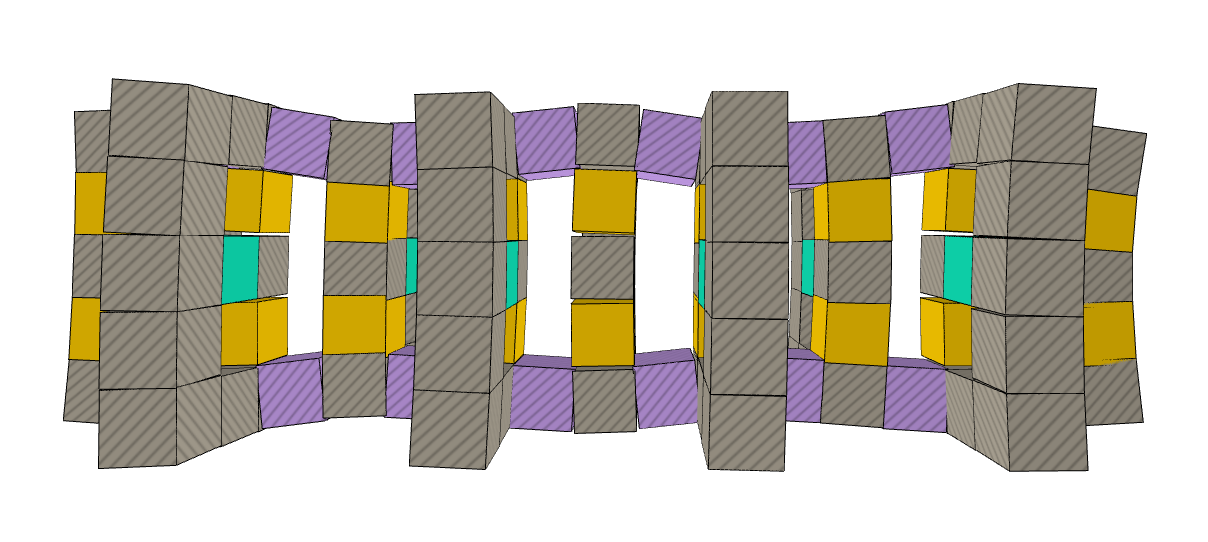
\includegraphics[width=\linewidth]{undulating.png}
  \caption{Undulating structure uses several stacks of linear actuators driven a third of a cycle out of phase from each other to create a sinusoidal motion up its spine.}
  \label{fig:undulating}
\end{figure}

%\include{DesignStudies}
%%% This is an example first chapter.  You should put chapter/appendix that you
%% write into a separate file, and add a line \include{yourfilename} to
%% main.tex, where `yourfilename.tex' is the name of the chapter/appendix file.
%% You can process specific files by typing their names in at the 
%% \files=
%% prompt when you run the file main.tex through LaTeX.

\singlespacing{

\chapter{Future Work}\label{chap:futureWork}

Future work revolves around hierarchical extensions of the current CAD/simulation model, experiments in computational design optimization, and development of a video game around digital materials.

\section{Hierarchical Simulation}

\begin{figure}
  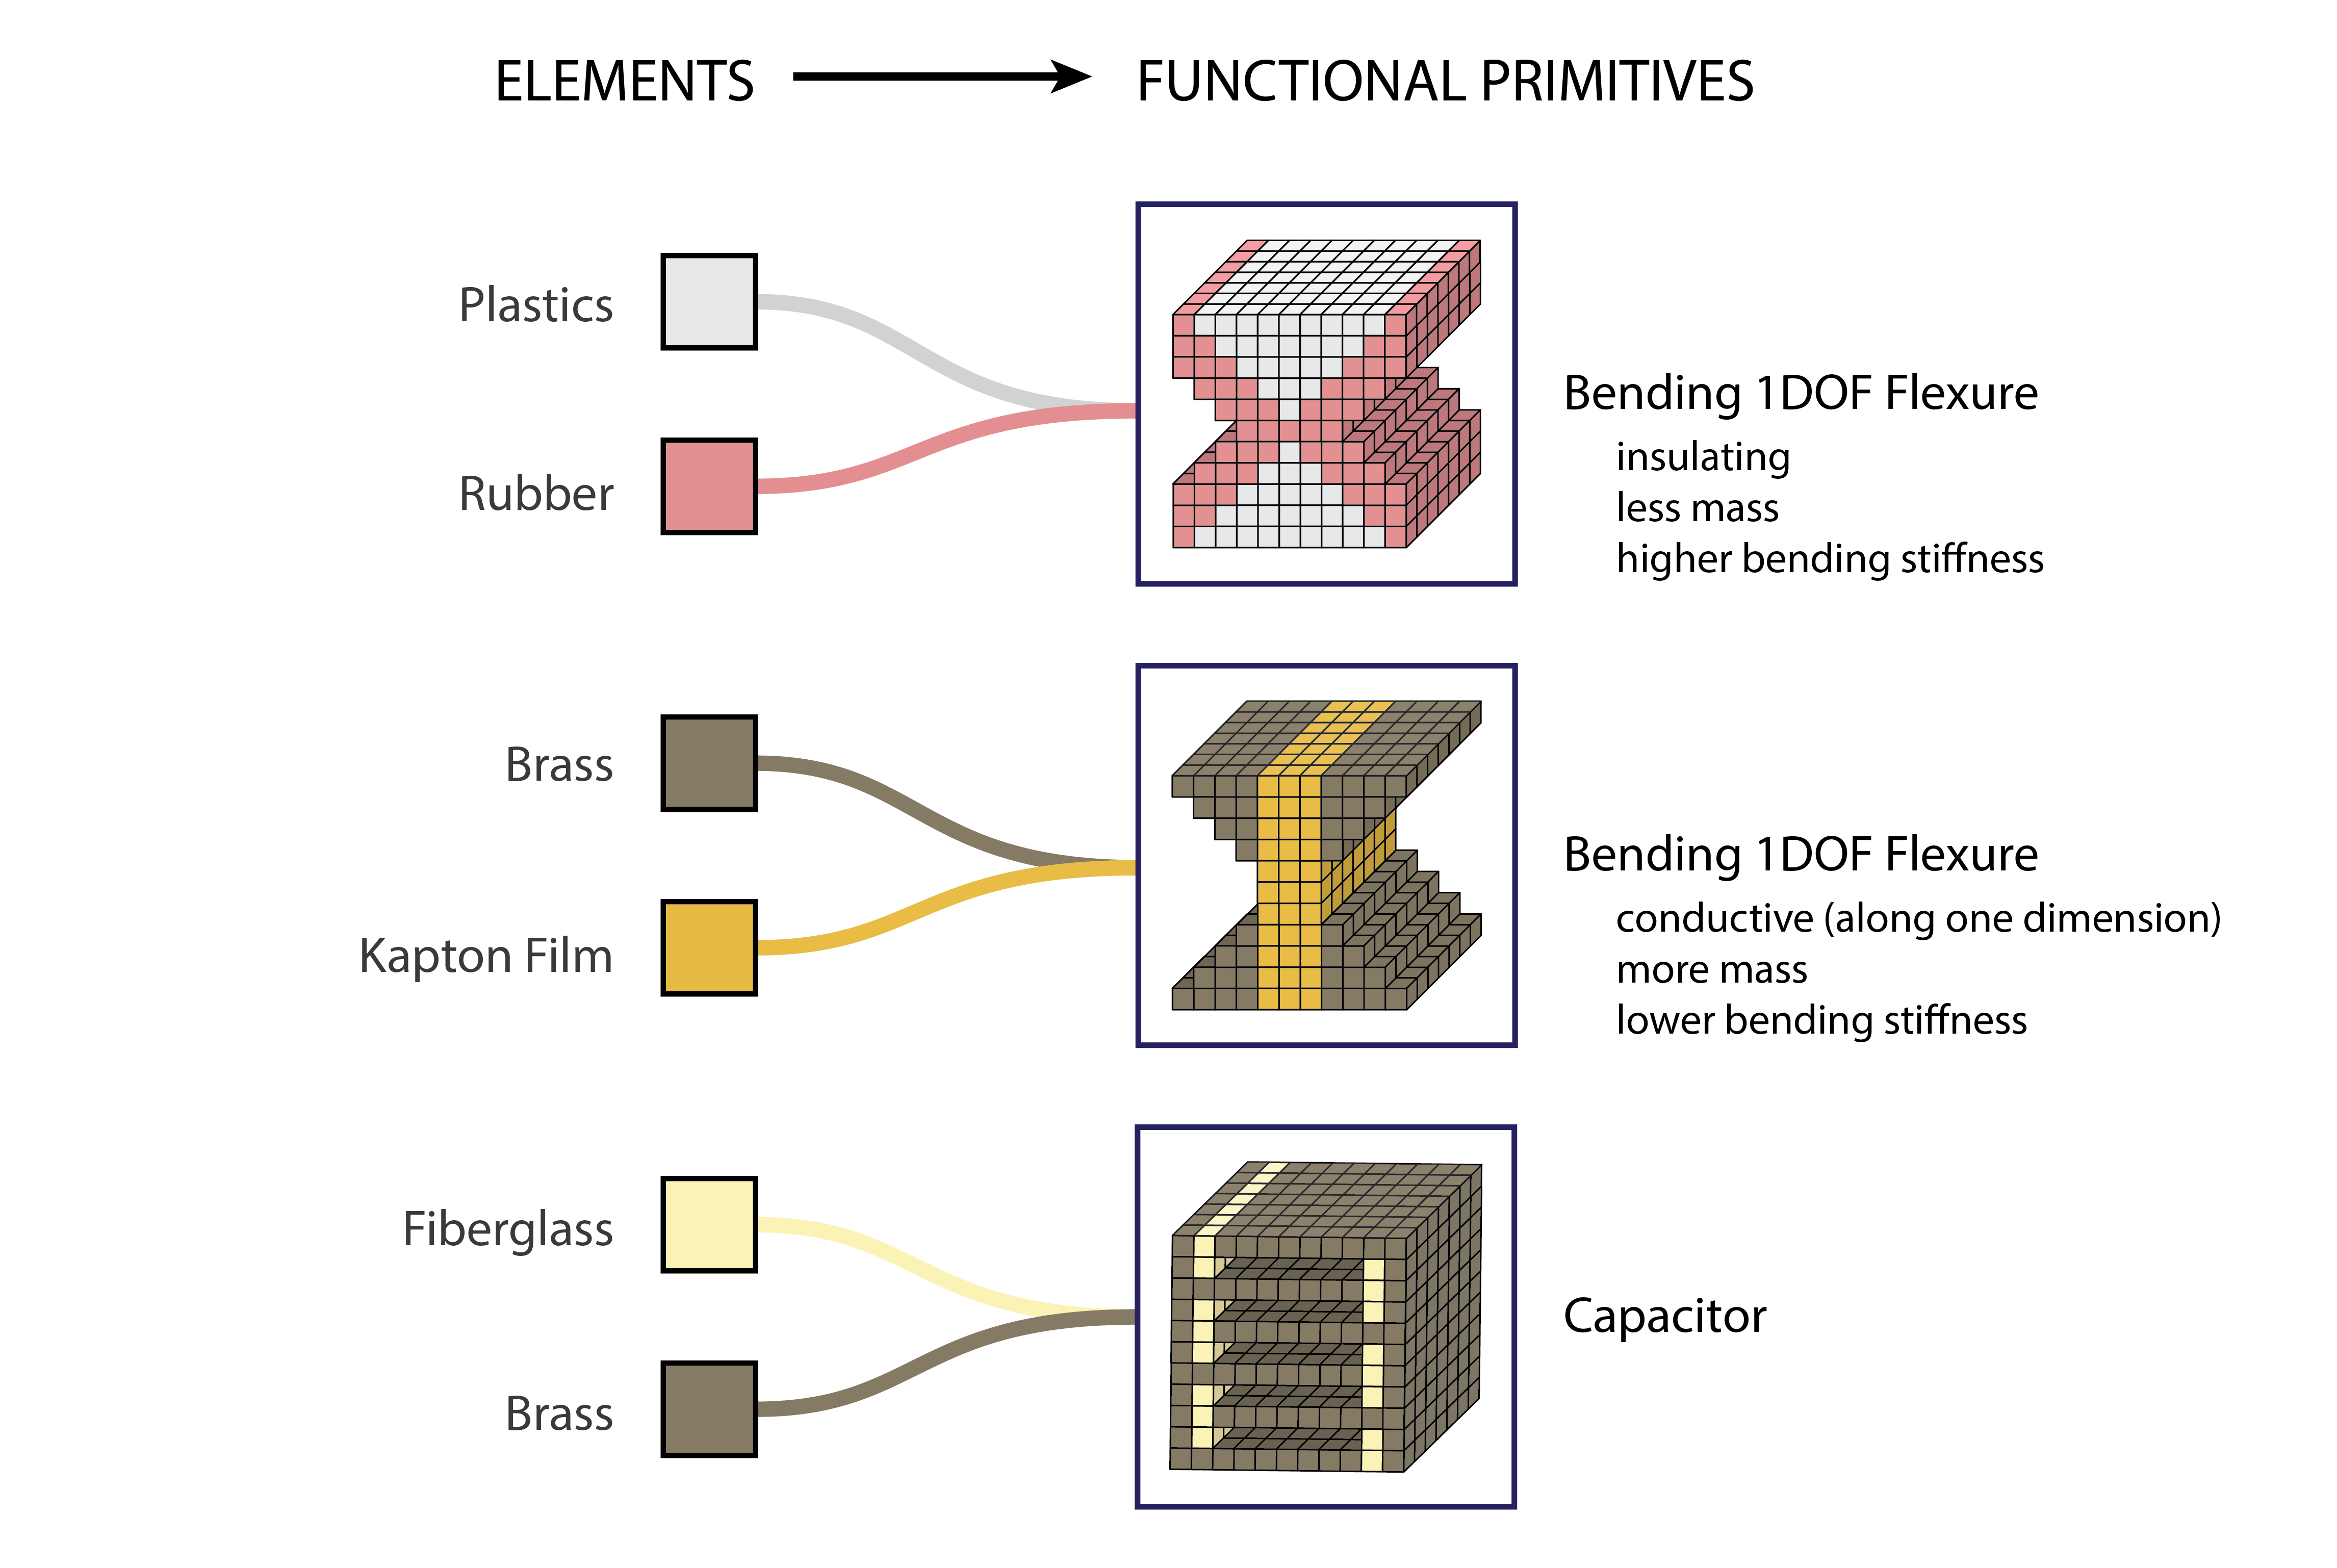
\includegraphics[width=\textwidth]{FunctionsParts.png}
  \caption{Three functional primitives decomposed as assemblies of elements.  The geometrical layout of elements within a functional primitive establish its mechanical and electronic properties.  Two sketches of a 1DOF Bending Flexure have different mass, moment of inertia, conductivity, and bending stiffnesses (top, middle).  Parallel plate construction of a capacitor from conducting and insulating parts determines the functional primitive's global capacitance (bottom).}
  \label{fig:FunctionsParts}
\end{figure}

The hierarchical scaling of structure and function in our assembly system (Chapter \ref{chapter:HierarchicalDesign}) hints to a hierarchical framing of design and simulation in software.  The bulk of this thesis explores CAD/simulation at the function-level, especially the decomposition of functional parts into functional primitives.  Future work will explore design and simulation at other levels of hierarchy and translate behaviors of assemblies at one level into higher-level building blocks.\\

Current thoughts around the translation of \textit{assemblies of elements} to \textit{functional primitives} are depicted in Figures \ref{fig:FunctionsParts} and \ref{fig:HierarchicalSim}.  Mechanical parameters describing a functional primitive are calculated from static simulations of assemblies of elements.  Boundary conditions applied to elements at each face of an assembly induce steady-state deformations; 15 sets of boundary conditions apply forces from which $F = kx$ and $T = k\theta$ may be solved for all 15 stiffness constants.  Additionally, the inertia tensor and mass are computed directly from constituent material densities and geometry.  For example, differences in composition between the two 1DOF bending flexures depicted in Figure \ref{fig:FunctionsParts} are expressed as differences in stiffness constants, mass, and inertia at the functional primitive level of description (Figure \ref{fig:HierarchicalSim}).  In the case that mechanical deformations are not linear over a range of applied forces, a constant $k$ is calculated to best fit the data.  \\

Electronic properties may be determined as well.  Conductance between faces of a functional primitive are trivially calculated from assemblies of conducting and insulating elements.  Static capacitance and inductance are computed using steady-state solutions to Finite Difference Time Domain (FDTD) simulations; previous work in DMDesign used FTDT to calculate potential fields (Figure \ref{fig:designAssemblyGUIWide}E).\\

\begin{figure}
  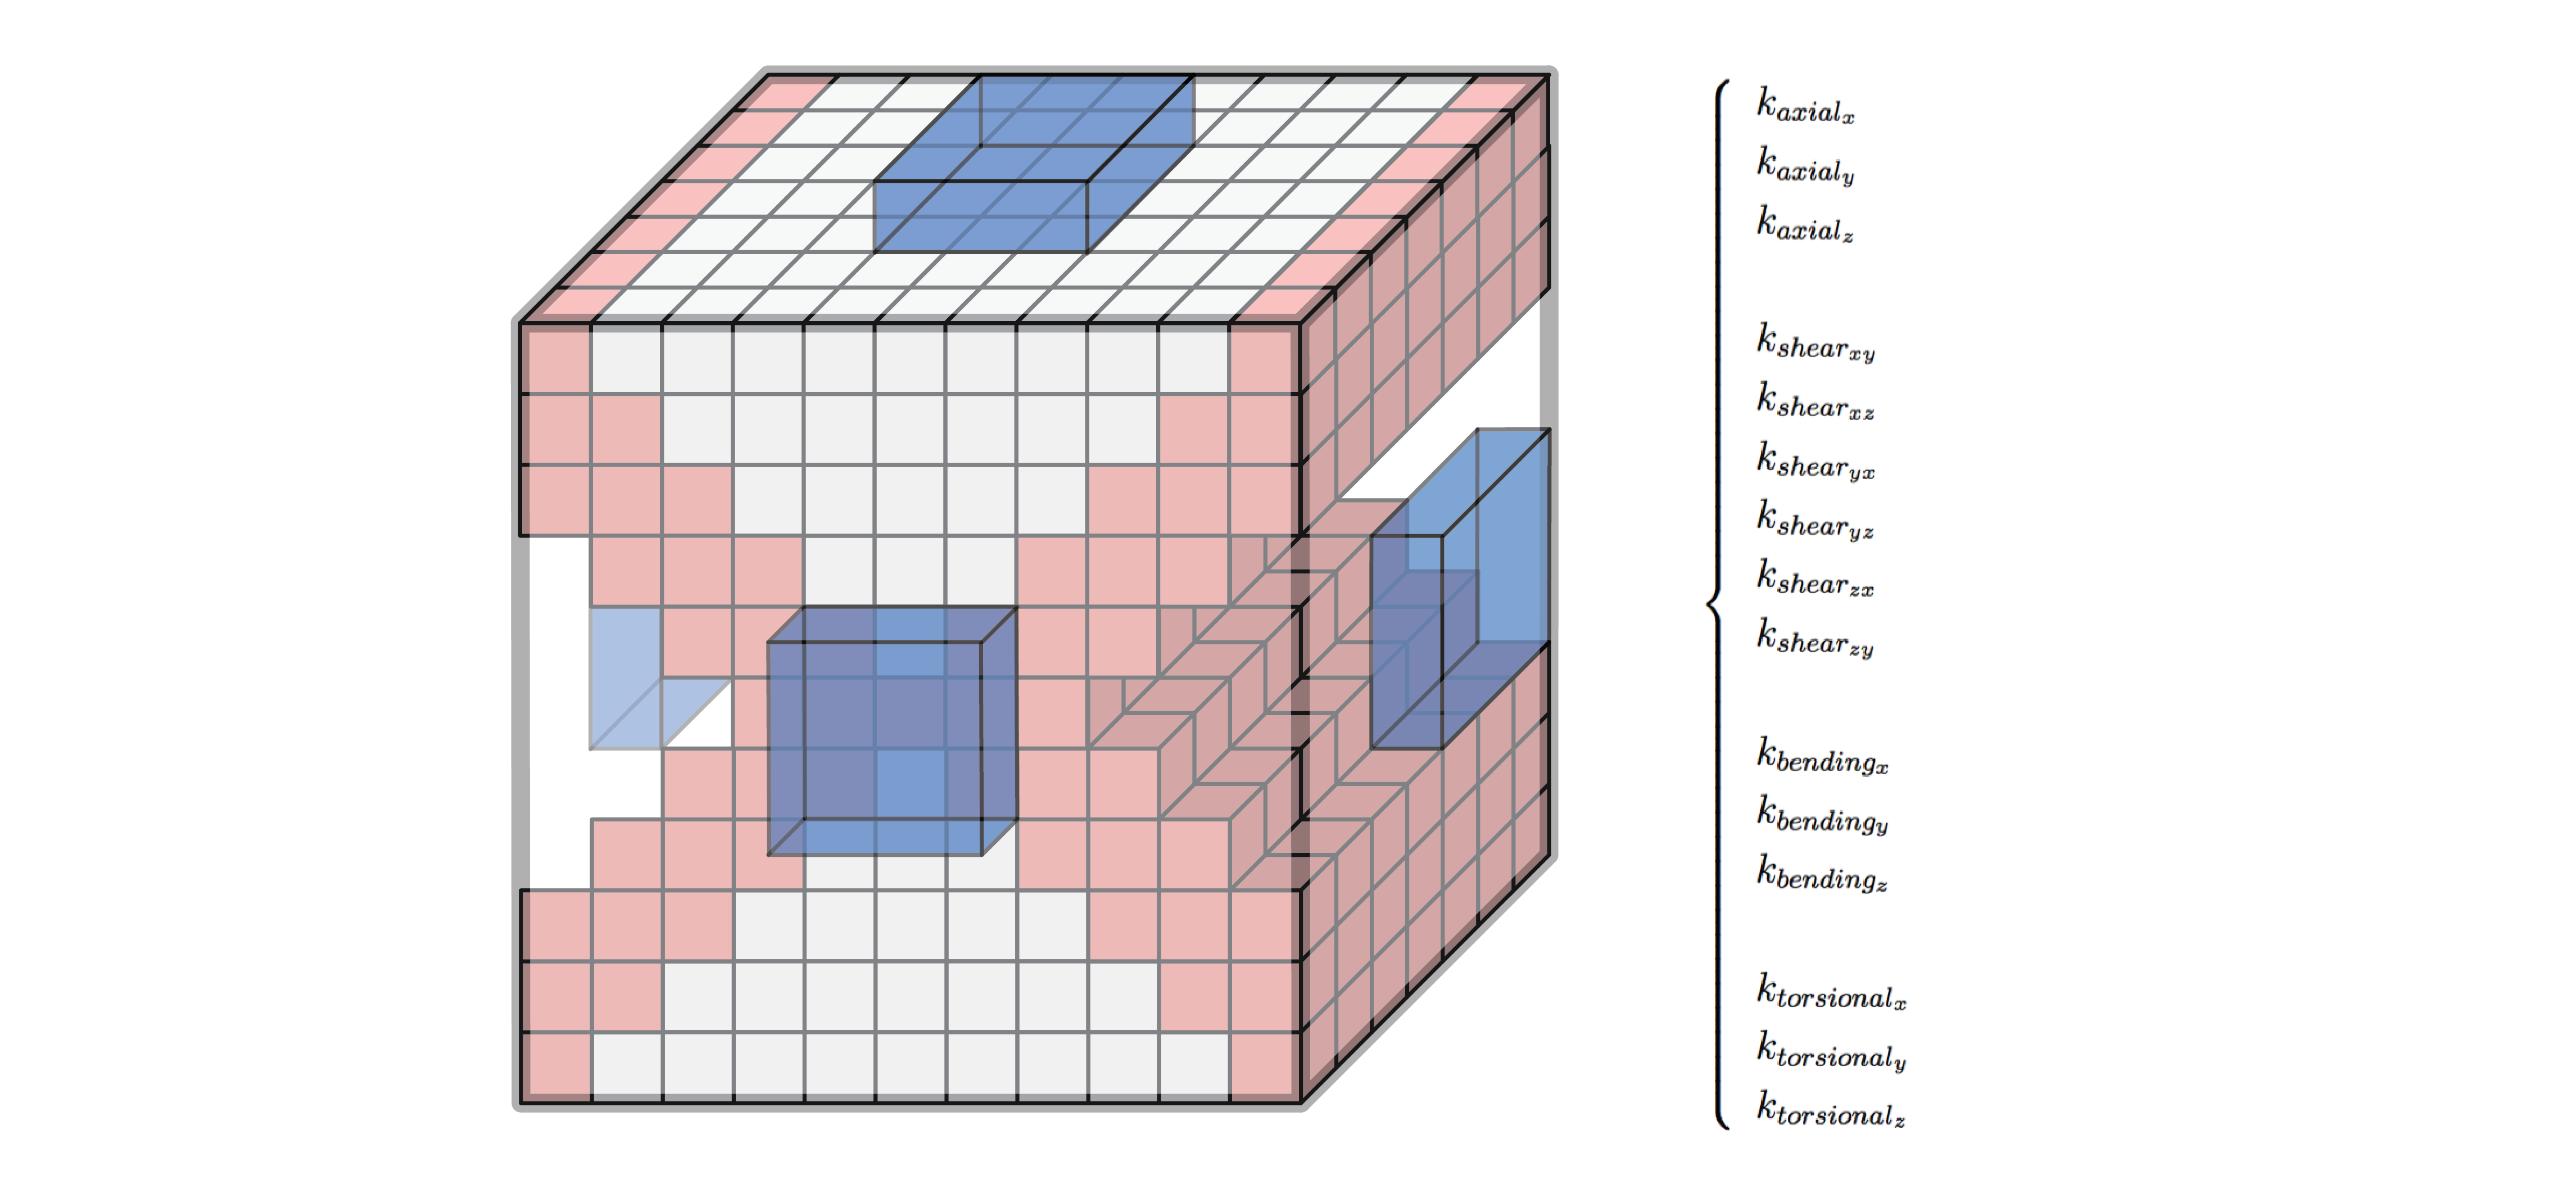
\includegraphics[width=\textwidth]{HierarchicalSim.png}
  \caption{Schematic view of the translation of an assembly of elements into functional primitive parameters: 15 stiffness constants, mass, and moment of inertia tensor.  Blue boxes indicate ``attachment points'' for applied boundary conditions in multidimensional stiffness measurements.}
  \label{fig:HierarchicalSim}
\end{figure}

Modules and complexes exhibit high-level behaviors that are abstracted from the low-level physics of the system.  Simulation of modules and complexes may reflect this abstraction by modeling interactions with a discretized, kinematic CA ruleset (somewhat like the work of William Stevens with CBlocks3D \cite{Stevens2009b}).  At this time it is still unclear how to generate a module's governing ruleset from behaviors of assemblies of function-level parts.

\section{Declarative Design}

A long term goal of this work is to close the loop between CAD and simulation and move towards \textit{declarative design}.  In a declarative design workflow, users specify high-level goals and a constrained optimization process searches across parameter space for a solution.  The discretization of space and finite set of parts types at each level hierarchy within our assembly system sets it up nicely for constrained design optimization.\\

Once a method of translating assemblies of elements into functional primitives has been established (see discussion from previous section), we can perform topology optimization across assemblies of elements to discover new types of functional primitives (Figure \ref{fig:DeclarativeDesign}).  Fabrication limitations should be translated into geometric constraints to ensure that the outcomes of the optimization are reasonable.  Future work could also explore optimization of control strategies for actuated assemblies, similar to previous work by Sims \cite{Sims1994}.

\begin{figure}
  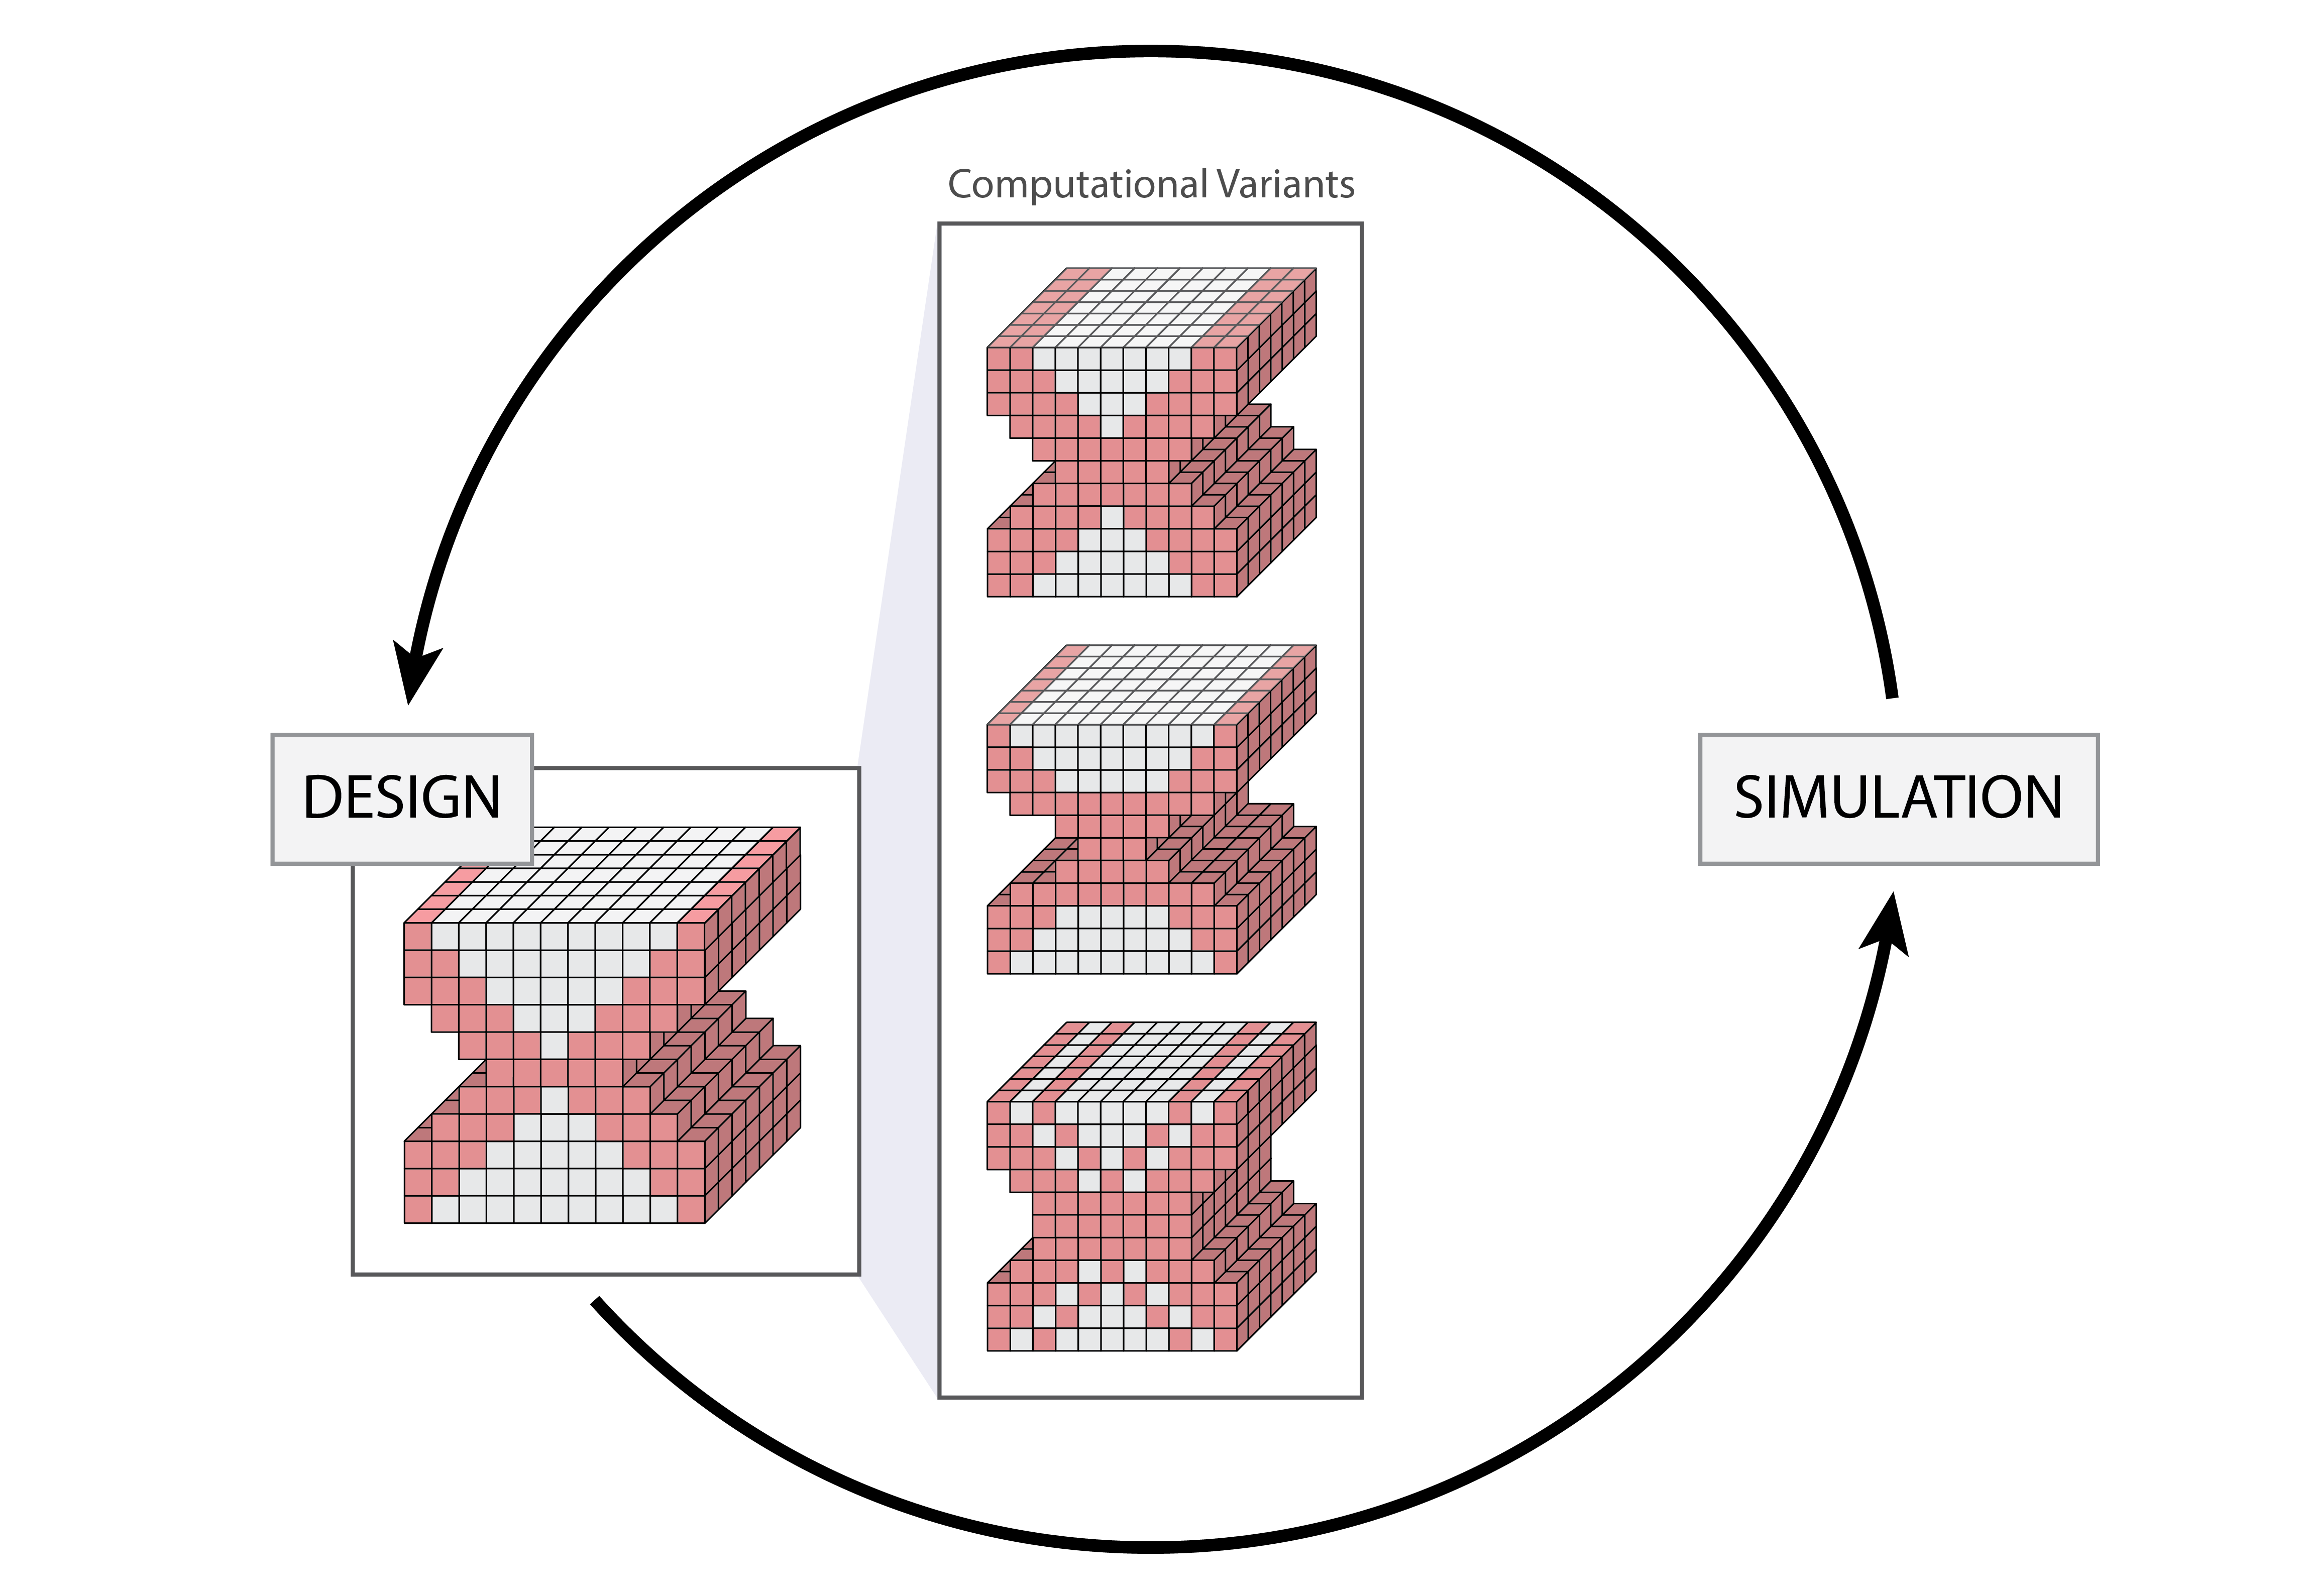
\includegraphics[width=\textwidth]{DeclarativeDesign.png}
  \caption{A 1DOF bending flexure is optimized in a topology optimization process.  Variations on initial user-generated design are evaluated in simulation.  This design/simulation loop is repeated until fabrication constraints and high-level goals are satisfied.}
  \label{fig:DeclarativeDesign}
\end{figure}

\section{``Fab the Game''}

An offshoot of the work described in this thesis is a collaboration with \href{http://elinemedia.com/}{E-Line Media} on a game.  Tentatively called ``Fab the Game'', it explores an aspirational future where digital materials are used to construct nearly everything.  In the game, players construct assemblies from functional primitives in an open-ended sandbox environment and in more directed challenges.  We envision a large component of gameplay revolves around constructing robots, operating them, and using them to shape the surrounding environment.\\

The game will extend the physical simulation outlined in Chapter \ref{chap:functionSim} through realtime user interaction.  For example, actuators in the game can be mapped to the keyboard and other gaming controllers so players can operate their robots in realtime.  Complex robots may be driven by a combination of preprogrammed controls and user input.  Using these controls, players test the agility and speed of their robot in arena challenges, drawing inspiration from the competitions of \href{http://www.firstinspires.org/robotics/frc}{First Robotics}.\\

More advanced modes of gameplay borrow from the ideas discussed in the previous two sections.  Players dive into functional primitive definitions and alter their elemental composition to unlock new functional properties beyond those available by default.\\

Through this game, we hope to familiarize players with CAD and simulation tools, constraint-based machine design, controls, and design optimization.  We will also provide offramps to digital fabrication workflows so that designs may be realized IRL (``in real life'') by gamers/makers.  In order to ease the burden of building large assemblies of parts, we may introduce concepts in hierarchical and parametric design within the crafting interface.  We are curious to see what players are able to construct within the game and hope it might inform future research trajectories at CBA.\\

Concept art by Eli Gershenfeld explores the look and feel of the game as well as potential gameplay scenarios (Figures \ref{fig:elibendy} through \ref{fig:elibridgefull}).

\clearpage

\begin{figure}
  \includegraphics[width=\textwidth]{elibendy.png}
  \caption{A swarm of locomoting robots.  \textit{Image Credit: Eli Gershenfeld 2016}}
  \label{fig:elibendy}
\end{figure}

\begin{figure}
  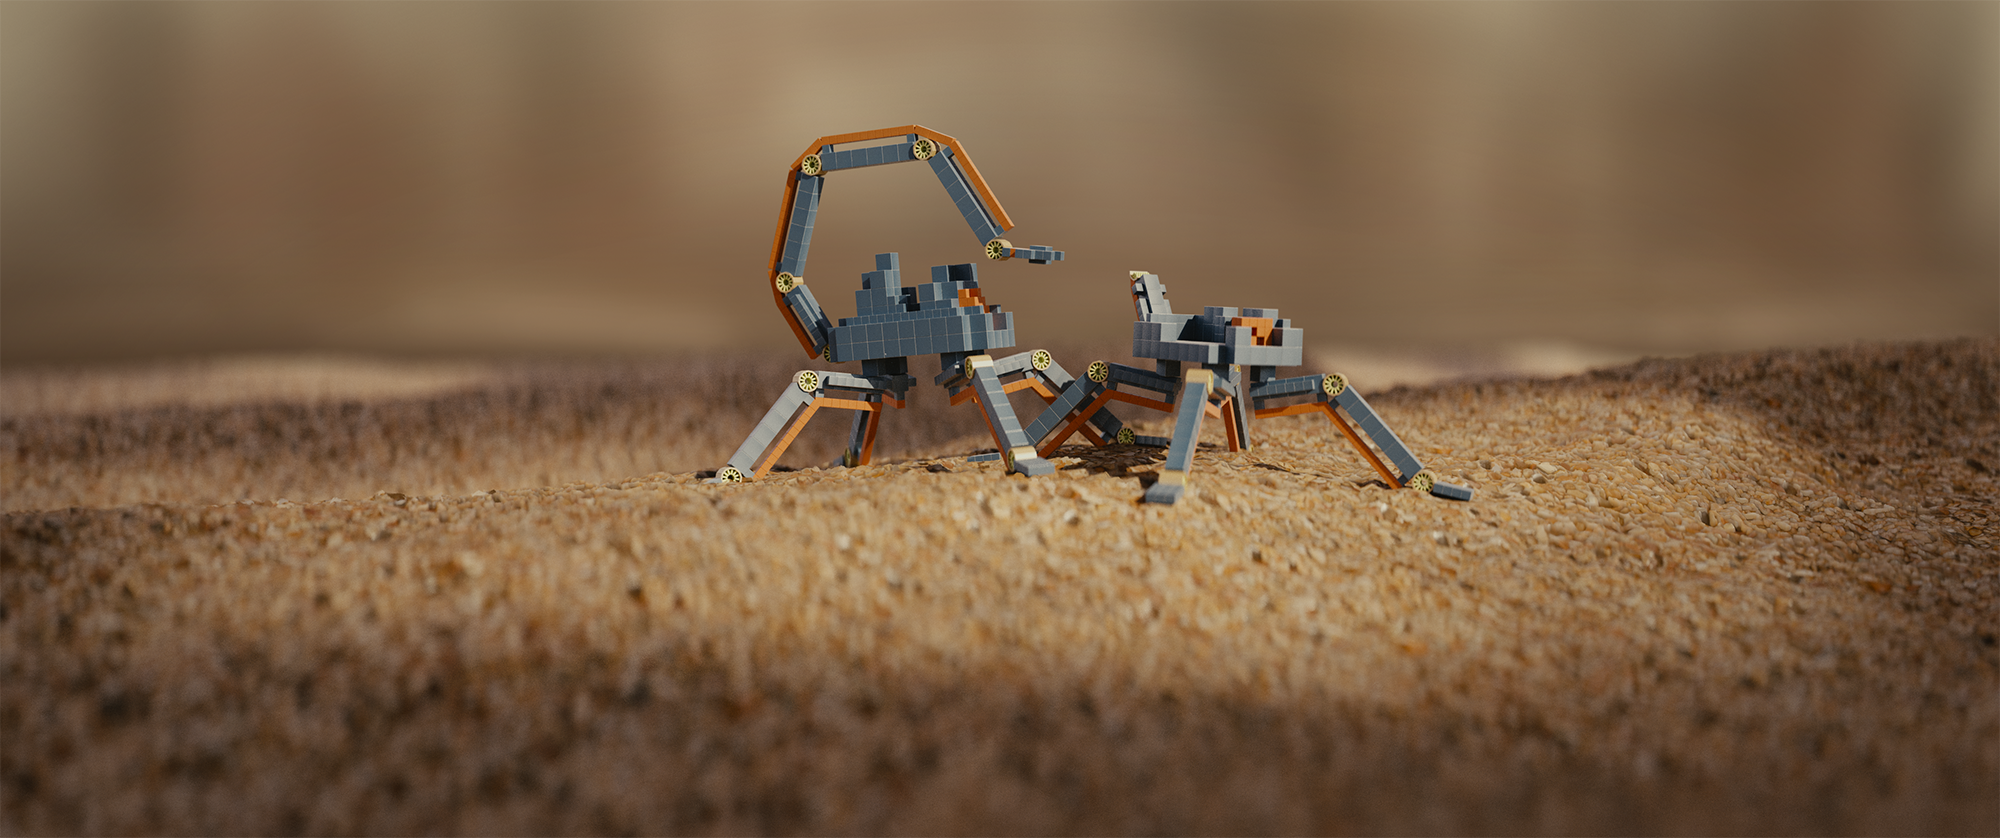
\includegraphics[width=\textwidth]{eliassemblers.png}
  \caption{Assembler assembling an assembler.  \textit{Image Credit: Eli Gershenfeld 2016}}
  \label{fig:eliassemblers}
\end{figure}

\begin{figure}
  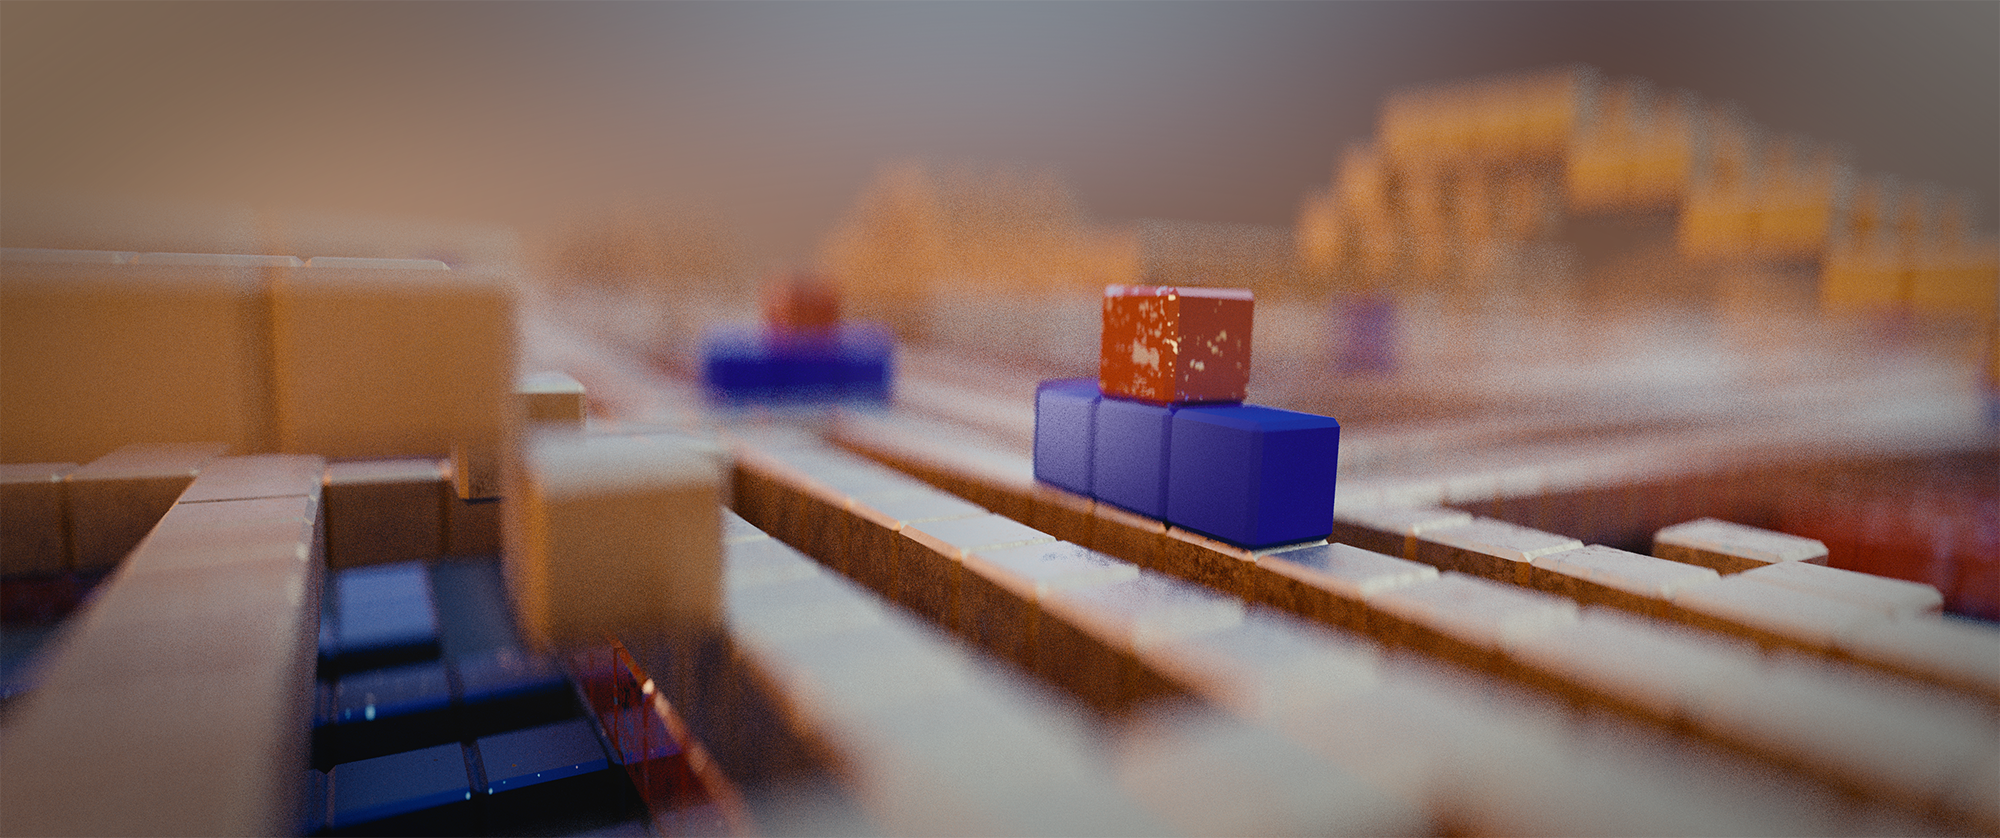
\includegraphics[width=\textwidth]{eliassembclose.png}
  \caption{Assembler ``factory'' feedstock.  \textit{Image Credit: Eli Gershenfeld 2016}}
  \label{fig:eliassembclose}
\end{figure}

\begin{figure}
  \includegraphics[width=\textwidth]{eliassembwide.png}
  \caption{Distributed ``factory'' automation. \textit{Image Credit: Eli Gershenfeld 2016}}
  \label{fig:eliassembwide}
\end{figure}

\begin{figure}
  \includegraphics[width=\textwidth]{elibridgeclose.png}
  \caption{``Living'' macro-scale structure.  \textit{Image Credit: Eli Gershenfeld 2016}}
  \label{fig:elibridgeclose}
\end{figure}

\begin{figure}
  \includegraphics[width=\textwidth]{elibridgefull.png}
  \caption{Self-assembling bridge. \textit{Image Credit: Eli Gershenfeld 2016}}
  \label{fig:elibridgefull}
\end{figure}


\appendix
%%% This is an example first chapter.  You should put chapter/appendix that you
%% write into a separate file, and add a line \include{yourfilename} to
%% main.tex, where `yourfilename.tex' is the name of the chapter/appendix file.
%% You can process specific files by typing their names in at the 
%% \files=
%% prompt when you run the file main.tex through LaTeX.

\singlespacing{

\chapter{Simulation Methods: Finite Difference, Finite Element, Finite Volume}

A differential equation is mathematical relationship between a function and at least one of its derivatives. For example:

 \begin{equation}\label{eq:diffEq}
 \frac{\partial^{2}f(x)}{\partial^{2}x} = f(x) + c
  \end{equation}
  \\
Equation \ref{eq:diffEq} describes a function $f$ with one independent variable $x$.  Differential equations of single variable functions like equation \ref{eq:diffEq} are called \textit{ordinary differential equations} (ODE).  A \textit{partial differential equation} (PDE) is a differential equation that describes multivariable functions.  PDEs are common in physics as many physical phenomena are dynamic in both space and time.

\section{PDEs from Physics}

\subsubsection{Heat Equation}

The \href{https://en.wikipedia.org/wiki/Heat_equation}{heat equation} describes the dissipation of heat through materials:

 \begin{equation}\label{eq:heatEq}
 \frac{\partial T}{\partial t} = c\nabla^{2}T
   \end{equation}
     \\
    where $t$ is time, $T$ is the temperature, $c$ is a constant, and $\nabla^{2}$ is the sum of the partial derivatives of $u$ with respect to the spatial dimensions of $u$ (also called the spatial \href{https://en.wikipedia.org/wiki/Laplace_operator}{Laplacian}).\\
    
    The heat equation contains a first derivative of $u$ with respect to $t$ and a second derivative of $u$ with respect to the spatial dimensions.  PDEs are classified based on the highest order derivative they contain, so the heat equation is a "second order" PDE.\\
    
     We can write a version of the heat equation for 1D(\ref{eq:heat1d}), 2D(\ref{eq:heat2d}), or 3D(\ref{eq:heat3d}) by expanding the Laplacian appropriately:
 
 \begin{equation}\label{eq:heat1d}
  \frac{\partial T}{\partial t} = c\frac{\partial^{2}T}{\partial^{2}x}
  \end{equation}
  
   \begin{equation}\label{eq:heat2d}
  \frac{\partial T}{\partial t} = c\left(\frac{\partial^{2}T}{\partial^{2}x}+\frac{\partial^{2}T}{\partial^{2}y}\right)
  \end{equation}
  
   \begin{equation}\label{eq:heat3d}
  \frac{\partial T}{ \partial t} = c\left(\frac{\partial^{2}T}{\partial^{2}x}+\frac{\partial^{2}T}{\partial^{2}y}+\frac{\partial^{2}T}{\partial^{2}z} \right)
  \end{equation}
  
\subsubsection{Wave Equation}

 The \href{https://en.wikipedia.org/wiki/Wave_equation}{wave equation} shows up often in physics - electricity and magnetism, acoustics, fluid dynamics, solid mechanics, etc.  It describes the propagation of waves through space and bears close resemblance to the heat equation:

 \begin{equation}\label{eq:waveEq}
 \frac{\partial^{2}u}{\partial^{2}t} = c\nabla^{2}u
   \end{equation}
     \\
 where $t$ is time, $u$ is the amplitude of the wave, $c$ is a constant, and $\nabla^{2}$ is the spatial Laplacian.  Like the heat equation (\ref{eq:heatEq}), this PDE is second order because it involves the second derivative of $u$ with respect to both $t$ and the spatial dimensions. \\
 
The 1D(\ref{eq:wave1d}), 2D(\ref{eq:wave2d}), or 3D(\ref{eq:wave3d}) expansions of the wave equation are given below:
 
 \begin{equation}\label{eq:wave1d}
  \frac{\partial^{2}u}{\partial^{2}t} = c\frac{\partial^{2}u}{\partial^{2}x}
  \end{equation}
  
   \begin{equation}\label{eq:wave2d}
  \frac{\partial^{2}u}{\partial^{2}t} = c\left(\frac{\partial^{2}u}{\partial^{2}x}+\frac{\partial^{2}u}{\partial^{2}y}\right)
  \end{equation}
  
   \begin{equation}\label{eq:wave3d}
  \frac{\partial^{2}u}{ \partial^{2}t} = c\left(\frac{\partial^{2}u}{\partial^{2}x}+\frac{\partial^{2}u}{\partial^{2}y}+\frac{\partial^{2}u}{\partial^{2}z} \right)
  \end{equation}
    
  \subsubsection{Advection Equation}
  
  The \href{https://en.wikipedia.org/wiki/Advection}{advection equation} describes the transport of material by a fluid, such as silt in a river:
  
   \begin{equation}\label{eq:advection}
  \frac{\partial s}{\partial t} = -v \cdot \frac{\partial s}{\partial x}
  \end{equation}
   \\
\section{Analytical vs Numerical Solutions}

Sometimes it's possible to find a continuous function that satisfies the relationships described by the PDE; this is refereed to as a \textit{closed-form} solution or \textit{analytical} solution.  Generally, this is the preferred form of the solution as it returns an exact value.\\

However, it is usually not possible to solve a PDE analytically, in these cases we must use numerical techniques to approximate the solution with a computer.  Generally, this involves splitting up, or \textit{discretizing}, space into a finite number of regions and evaluating the PDE in each of these regions.  Often this process of discretization is applied to time as well, creating a solution that moves forward in quantized time steps.  As the size of the spatial regions and temporal steps becomes very small, the discrete solution approaches the continuous, analytical solution to the PDE.

\section{Finite Difference Method}

We'll start with an arbitrary continuous, differentiable function $f(x)$.  If we know some $f(x_{0})$, we can estimate $f(x_{0}+\Delta  x)$ with the Taylor Series expansion.  The n degree Taylor Series expansion around $f(x_{0})$ is given by:

 \begin{equation}\label{eq:norderTaylor}
  f(x_{0} + \Delta  x) = f(x_{0}) + \frac{f'(x_{0})}{1!}\Delta  x + \frac{f''(x_{0})}{2!}\Delta  x^{2} + \cdots  + \frac{f^{(n)}(x_{0})}{n!}\Delta  x^{n} + R_{n}(x_{0})
  \end{equation}
    \\
  where $f^{(n)}(x_{0})$ is the $n$th derivative of $f(x)$ evaluated at $x_{0}$ with respect to $x$ and $R_{n}(x_{0})$ is a remainder error term that depends on the degree of the Taylor expansion.  The Taylor expansion is not an approximation, it returns the exact value of $ f(x_{0} + \Delta  x)$.  As $n$ approaches infinity, $R_{n}(x_{0})$ vanishes.\\
  
%   \begin{equation}
%   \lim_{n \to \infty} R_{n}(x_{0}) = 0
%   \end{equation}

A first order Taylor expansion reduces \ref{eq:norderTaylor} to:
  
 \begin{equation}\label{eq:1degTaylor}
  f(x_{0} + \Delta  x) = f(x_{0}) + f'(x_{0})\Delta x + R_{1}(x_{0})
  \end{equation}
    \\
  For small $\Delta  x$ it is OK to ignore the error term.  We are left with a first order Taylor approximation:
  
   \begin{equation}\label{eq:1degTaylorApprox}
  f(x_{0} + \Delta  x) \approx f(x_{0}) + f'(x_{0})\Delta x
  \end{equation}
    \\
This is the same as tracing the slope of $f$ at $x_{0}$ to approximate a nearby value.  Rearranging \ref{eq:1degTaylorApprox} gives us an expression for the first derivative of $f(x)$ with respect to $x$:

 \begin{equation}\label{eq:fdaForward}
 f'(x_{0}) \approx \frac{f(x_{0} + \Delta  x) - f(x_{0})}{\Delta  x}
  \end{equation}
    \\
Similarly, we can evaluate the first order Taylor approximation for negative $\Delta x$:

     \begin{equation}
 f(x_{0} - \Delta  x) \approx f(x_{0}) - f'(x_{0})\Delta x
  \end{equation}
    \\
  Rearranging this gives us an alternate form of $ f'(x_{0})$:

 \begin{equation}\label{eq:fdaBackward}
 f'(x_{0}) \approx \frac{f(x_{0}) - f(x_{0} - \Delta  x)}{\Delta  x}
  \end{equation}
    \\
Summing equations \ref{eq:fdaForward} and \ref{eq:fdaBackward} gives yet another form:
  
     \begin{equation}\label{eq:fdaCentered}
 f'(x_{0}) \approx \frac{f(x_{0} + \Delta  x) - f(x_{0} - \Delta  x)}{2\Delta x}
  \end{equation}
  \\
  Equations \ref{eq:fdaForward}, \ref{eq:fdaBackward}, \ref{eq:fdaCentered} are referred to as the first order forward, backward, and centered finite difference approximations.  We can use these as approximations to first order derivatives in a PDE so that the PDE can be rewritten in a form that is easy to solve.
  
\subsection{Example of First Order FDM}



\subsection{Higher Order FDM}

In order to solve a second order PDE like the wave equation (\ref{eq:waveEq}), we'll need a finite difference approximation for second derivatives.  We found the first order finite difference approximations by rearranging the first order Taylor approximation (\ref{eq:1degTaylorApprox}); this time, we'll start with a second order Taylor expansion of the full Taylor Series (\ref{eq:norderTaylor}):

 \begin{equation}
  f(x_{0} + \Delta  x) = f(x_{0}) + f'(x_{0})\Delta  x + \frac{f''(x_{0})}{2}\Delta  x^{2} + R_{n}(x_{0})
  \end{equation}
    \\
  Again, for small $\Delta  x$, we can ignore the error term to get the second order Taylor approximation:
  
   \begin{equation}\label{eq:secOrderTaylorApprox}
  f(x_{0} + \Delta  x) \approx f(x_{0}) + f'(x_{0})\Delta  x + \frac{f''(x_{0})}{2}\Delta  x^{2}
  \end{equation}
    \\
  And similarly for  $f(x_{0} - \Delta  x)$:
  
     \begin{equation}\label{eq:secOrderTaylorApproxNeg}
  f(x_{0} - \Delta  x) \approx f(x_{0}) - f'(x_{0})\Delta  x + \frac{f''(x_{0})}{2}\Delta  x^{2}
  \end{equation}
    \\
  Adding equations \ref{eq:secOrderTaylorApprox} and \ref{eq:secOrderTaylorApproxNeg} cancels out the $f'(x_{0})$ terms:
  
   \begin{equation}
  f(x_{0} + \Delta  x) + f(x_{0} - \Delta  x) \approx 2f(x_{0}) + f''(x_{0})\Delta  x^{2}
  \end{equation}
    \\
  Rearranging gives us the centered second order finite differential approximation:
  
   \begin{equation}
   f''(x_{0}) \approx \frac{f(x_{0} + \Delta  x) - 2f(x_{0}) + f'(x_{0} -\Delta  x)}{\Delta  x^{2}}
  \end{equation}
    \\
  The forward second order finite differential approximation requires equation \ref{eq:secOrderTaylorApprox} and an approximation of $f'(x_{0} + 2\Delta  x)$:
  
  \begin{equation}\label{eq:secOrderTaylorApprox2}
  f(x_{0} + 2\Delta  x) \approx f(x_{0}) + f'(x_{0})2\Delta  x + \frac{f''(x_{0})}{2}4\Delta  x^{2}
  \end{equation}
    \\
  Subtracting 2x equation \ref{eq:secOrderTaylorApprox} from \ref{eq:secOrderTaylorApprox2} gives:
  
    \begin{equation}
  f(x_{0} + 2\Delta  x) - 2f(x_{0} + \Delta  x) \approx -f(x_{0}) + f''(x_{0})\Delta  x^{2}
  \end{equation}
  \\
Which simplifies to the forward second order finite differential approximation:
  
      \begin{equation}
f''(x_{0}) \approx \frac{f(x_{0} + 2\Delta  x) - 2f(x_{0} + \Delta  x) + f(x_{0})}{\Delta  x^{2}}
  \end{equation}
  \\
  The backward second order finite differential approximation is calculated similarly:
  
        \begin{equation}
f''(x_{0}) \approx \frac{f(x_{0} - 2\Delta  x) - 2f(x_{0} - \Delta  x) + f(x_{0})}{\Delta  x^{2}}
  \end{equation}
  \\
 Beyond this, higher order finite differential approximations may be calculated similarly, or from the following general forms of the forward (\ref{eq:generalFDAForward}), backward (\ref{eq:generalFDABackward}), and center (\ref{eq:generalFDACenter}) $n$th order finite difference approximations:
 
  \begin{equation}\label{eq:generalFDAForward}
 f^{n}(x_{0}) = \frac{1}{\Delta  x^{n}}\sum_{i=0}^{n}(-1)^{i}\binom {n} {i}f(x_{0} + (n-i)\Delta  x)
 \end{equation}
 
 \begin{equation}\label{eq:generalFDABackward}
 f^{n}(x_{0}) = \frac{1}{\Delta  x^{n}}\sum_{i=0}^{n}(-1)^{i}\binom {n} {i}f(x_{0} - i\Delta  x)
 \end{equation}
 
  \begin{equation}\label{eq:generalFDACenter}
 f^{n}(x_{0}) = \frac{1}{\Delta  x^{n}}\sum_{i=0}^{n}(-1)^{i}\binom {n} {i}f(x_{0} + \left(\frac{n}{2}-i\right)\Delta  x)
 \end{equation}
 \\
\subsection{Example of Second Order FDM}

Now that we have a second order finite difference approximation, we can solve second order PDEs numerically with FDM.  The 1D wave equation \ref{eq:wave1d}, whose solution is given by a function $u(t, x)$, is re-written using the second order centered finite difference approximation(\ref{eq:fdasecondcentered}) in space and the backward finite difference approximation in time(\ref{eq:fdasecondbackward}):

 \begin{equation}
 \begin{split}
  \frac{u(t_{0} + \Delta  t, x_{0}) - 2u(t_{0}, x_{0}) +u(t_{0} - \Delta  t, x_{0})}{\Delta  t^{2}}\\
 = c  \frac{u(t_0, x_{0} + \Delta  x) - 2u(t_0, x_{0}) +u(t_0, x_{0} - \Delta  x) }{\Delta  x^{2}}
 \end{split}
  \end{equation}

\subsection{FDM as a Cellular Automata Ruleset}


A longer discussion and additional examples of this method are given in Yang et al\cite{Yang2010}.

\subsection{Example Code}

\subsection{Error Analysis}

 \begin{equation}
 f'(x_{0}) = \frac{f(x_{0} + \Delta  x) - f(x_{0})}{\Delta  x} + \frac{R_{1}(x_{0})}{\Delta  x}
  \end{equation}
  
For small changes $\Delta  x$ in the negative direction, equation  can be rearranged to:

 \begin{equation}
 f'(x_{0}) = \frac{f(x_{0}) - f(x_{0} - \Delta  x)}{\Delta  x} - \frac{R_{1}(x_{0})}{\Delta  x}
  \end{equation}
  
  fjalsdjflkadsjf
  
   \begin{equation}
 f'(x_{0}) = \frac{f(x_{0} + \Delta  x) - f(x_{0} - \Delta  x)}{2\Delta x} + \frac{R_{1}(x_{0})}{2\Delta  x}
  \end{equation}
  
\section{Differential vs Integral Forms}
\section{Finite Element Method}

\section{Finite Volume Method}

%\include{DesignFiles}
%%% This defines the bibliography file (main.bib) and the bibliography style.
%% If you want to create a bibliography file by hand, change the contents of
%% this file to a `thebibliography' environment.  For more information 
%% see section 4.3 of the LaTeX manual.
\begin{singlespace}
\renewcommand{\bibname}{External Media}
\begin{thebibliography}{1}

\bibitem{jifei}
\href{http://ou-jifei.com/}{Jifei Ou personal website}.  Images of multimaterial Objet print taken from \href{https://vimeo.com/127666944#t=89s}{Autodesk Pier 9 video}.

\bibitem{objet}
\href{http://www.stratasys.com/3d-printers/production-series/connex3-systems}{Objet Connex Multimaterial 3D Printer website}

\bibitem{minecraft}
\href{https://minecraft.net/}{Official Minecraft website}

\bibitem{redstoneCircuit}
\href{http://minecraft.gamepedia.com/Redstone_circuit}{Redstone Circuit - Minecraft Wiki}

\end{thebibliography}
\end{singlespace}

%%% This defines the bibliography file (main.bib) and the bibliography style.
%% If you want to create a bibliography file by hand, change the contents of
%% this file to a `thebibliography' environment.  For more information 
%% see section 4.3 of the LaTeX manual.
\begin{singlespace}
\renewcommand{\bibname}{References}
\bibliography{mendeley/ThesisWURL}
\bibliographystyle{customBibStyle}
\end{singlespace}

\end{document}


